\documentclass[10pt]{project}


\definecolor{color1}{RGB}{0,0,90}
\definecolor{color2}{RGB}{0,20,20}

\usepackage{tcolorbox,listings,multirow,placeins,tikz,pgf,pdfpages, lipsum, pdflscape, pgfgantt,float, subfigure,amsmath,lscape}
\usepackage[normalem]{ulem}
\usepackage[hyphens]{url}

\usepackage{gensymb}

\usetikzlibrary{shapes.geometric, arrows,shapes,positioning,shadows,trees}

\useunder{\uline}{\ul}{}

\tikzstyle{process} = [rectangle, minimum width=3cm, minimum height=1cm, text centered, draw=black, fill=blue!30]
\tikzstyle{arrow} = [thick,->,>=stealth]

\tikzset{
every node/.style={draw,text width=2cm,drop shadow},
style1/.style= {rectangle, rounded corners=2pt, thin,align=center,fill=green!30},
style2/.style= {rectangle, rounded corners=6pt, thin,align=center,fill=green!60},
style3/.style= {rectangle,thin,align=left,fill=pink!60}
}

\lstset{
	showstringspaces=false,
  tabsize=2,
  breaklines=true,
  columns=fullflexible
}
\tcbuselibrary{breakable}

\usepackage{hyperref}
\hypersetup{hidelinks,colorlinks,breaklinks=true,urlcolor=color2,citecolor=color1,linkcolor=color1,bookmarksopen=false,pdftitle={Title},pdfauthor={Author}}

\JournalInfo{

\includegraphics[width=2.5cm]{Figures/engineering-logo}
\Archive{}
}

\PaperTitle{Mandan Refinery Senior Design Project}

\Authors{Benedict Brophy\textsuperscript{1}*,
Gannon Steffes\textsuperscript{1}**,
Jonathan Ganzer\textsuperscript{1}***,
Jacob Ganzer\textsuperscript{1}****.}
\affiliation{\textsuperscript{1}\textit{Engineering, 
  University of Mary, Bismarck, North Dakota}}
\affiliation{*bbrophy1@umary.edu}
\affiliation{**grsteffes1@umary.edu}
\affiliation{***jmganzer1@umary.edu}
\affiliation{****jnganzer1@umary.edu}

\Keywords{}
\newcommand{\keywordname}{Keywords}
\Abstract{This report covers the design for an improved system of unloading a 2000-lb bulk bag of calcium chloride for the Mandan Refinery.  The improved design aims to increase the usability and reliability of the structure while maintaining a strong emphasis on safety for the operator.  This report covers all the necessary background information for the project, initial concepts, and justification for the final design choices.}
%Give a one-paragraph summary of the whole document.
\begin{document}

\raggedbottom
\maketitle
\tableofcontents
\thispagestyle{empty}

\section{Introduction}
The Mandan Refinery Senior Design Project aims to improve the efficiency and safety of unloading and processing calcium chloride ($CaCl_2$) at the Marathon Oil Refinery in Mandan, North Dakota. The current bulk bag unloader presents challenges in ergonomics, material flow, and mixing, making it difficult for operators to handle 2000-lb bags effectively. Additionally, inadequate mixing in the neutralization pit leads to clumping of $CaCl_2$ and inefficiencies in the process. This project focuses on redesigning the unloading mechanism to allow for safer and more efficient handling of $CaCl_2$ while implementing an improved mixing solution to enhance dissolution.

\begin{figure}[H]
    \centering
    
\includegraphics[width=1\linewidth]{Senior Design Project Template//Figures/BulkBagUnloader.PNG}
    \caption{Current Bulk Bag Unloader at the Marathon - Mandan Refinery.  The current system is too tall for the operators to use safely.\cite{Marathon}}
    \label{fig:BulkBagUnloader}
\end{figure}

\newpage
\subsection{Statement of Project Qualifications}\label{sec:pq}

For this project, it is important to first define the scope of the project, as well as define the necessary design constraints.  Table \ref{tab:pq} explains what the scope of this project is, what is expected from this report, and lists the constraints that will be operated under.  Assignments are also given to each member of the group, along with their individual responsibilities.

%The statement of project qualifications gives an overall description of the project scope and all of its requirements while including any constraints or extra criteria needed. It defines each member and their general roles in the project. 

% Please add the following required packages to your document preamble:
% \usepackage[table,xcdraw]{xcolor}
% Beamer presentation requires \usepackage{colortbl} instead of \usepackage[table,xcdraw]{xcolor}
\begin{table}[H]
\begin{centering}
\begin{tabular}{|ll|}
\hline
\multicolumn{1}{|l|}{{\color[HTML]{FF0000} Mandan Refinery Senior Design Project}}                     &                                                                                                                                                                                                                                                                                                                                                                                                                                                                                                            \\ \hline
\multicolumn{1}{|l|}{{\color[HTML]{FF0000} Project Members}}                  &  Benedict Brophy, Gannon Steffes, Jonathan Ganzer, Jacob Ganzer                                                                                                                                                                                                                                                                                                               \\ \hline
\multicolumn{1}{|l|}{{\color[HTML]{FF0000} Stakeholders}}                     & \begin{tabular}[c]{@{}l@{}}Marathon Oil Refinery, Located in Mandan North Dakota\end{tabular} \\ \hline
\multicolumn{1}{|l|}{{\color[HTML]{FF0000} Project Purpose}}                  & \begin{tabular}[c]{@{}l@{}} This project aims to modify the existing bulk bag unloader at the south end of the \\Mandan Marathon Oil Refinery to facilitate safer and more efficient operation.\end{tabular}                                                   \\ \hline
\multicolumn{1}{|l|}{{\color[HTML]{FF0000} Description}}                      & \begin{tabular}[c]{@{}l@{}} The Mandan Refinery proposes a project to redesign the existing bulk bag\\
unloader at the Alkylation unit. The bulk bag unloader is utilized to route solid\\
pellets of $CaCl_2$ to the neutralization pit. The pellets are unloaded into the\\
neutralization pit using 2000-lb bags. These bags are designed to be loaded via\\
telehandler to the top of the bulk bag unloader. The bag is mounted on four\\
mounting legs at the top of the bulk bag unloader. The bottom of the 2000-lb\\
bag is opened up and fed into the neutralization pit via a slide valve and metal\\
chute. Currently, the bulk bag unloader setup does not allow operators to\\
ergonomically unload the 2000-pound bags using loading equipment. The\\
mounting legs are difficult to get the 2000-lb bags placed on. Additionally,\\
the solid $CaCl_2$ does not mix adequately once it is released into the\\
neutralization pit. This is due to inadequate mixing mechanisms within the\\
existing neutralization pit. \end{tabular}                                                                      \\ \hline
\multicolumn{1}{|l|}{{\color[HTML]{FF0000} Desired Results}}                  & \begin{tabular}[c]{@{}l@{}}- Design a mechanism to safely load the 2000-lb $CaCl_2$ bags into the neutralization pit.\\ - Design a mixing method for the neutralization pit to reduce clumping of $CaCl_2$. 
\end{tabular}                                                                                                                                                                                                                                                                                                                     \\ \hline
\multicolumn{1}{|l|}{{\color[HTML]{FF0000} Exclusions}}                       & \begin{tabular}[c]{@{}l@{}}A prototype of any kind shall not be included in the scope of this project. \end{tabular}                                                                                                                                                                                                                                                                                \\ \hline
\multicolumn{1}{|l|}{{\color[HTML]{FF0000} Communication Needs}}              & \begin{tabular}[c]{@{}l@{}}Project members shall be in contact at all times with each other and shall meet on\\ an as needed basis with Marathon Oil. Weekly meetings with Marathon Oil\\ will be included as checkpoints for both the design team and Marathon staff. \end{tabular}                                                                                                                                                                                                                                                                                                                    \\ \hline
\multicolumn{1}{|l|}{{\color[HTML]{FF0000} Acceptance Criteria}}              & \begin{tabular}[c]{@{}l@{}} The acceptance of this project shall be determined by the course instructors\\ and the engineers at Marathon.\end{tabular}                                                                                                                                                                                                                                                                                                         \\ \hline
\multicolumn{1}{|l|}{{\color[HTML]{FF0000} Constraints}}                      & \begin{tabular}[c]{@{}l@{}} The primary constraint is safely. Safety shall be held to the highest\\
priority over all other constraints. The design is constricted to a limited\\ footprint of 15'x 12'8" at the design site and is limited by the existing\\design of the bulk bag unloader. \end{tabular}                                                                                                                    \\ \hline
\multicolumn{2}{|c|}{{\color[HTML]{FF0000} High-Level Assignments}}     \\ \hline

\multicolumn{1}{|l|}{{\color[HTML]{FF0000} Benedict Brophy}} & \begin{tabular}[c]{@{}l@{}} Electrical Engineer - Responsible for creating electrical schematic via AutoCAD. \\ Will work with Gannon on all aspects of electrical design.     \end{tabular} \\ \hline

\multicolumn{1}{|l|}{{\color[HTML]{FF0000} Gannon Steffes}} & \begin{tabular}[c]{@{}l@{}} Electrical Engineer - Managerial/EE role. The primary form of contact for Marathon \\
engineers and typically assigns tasks to group members. Will work with Ben\\
on all aspects of electrical design. Responsible for maintaining electrical\\ 
code standards. \end{tabular} \\ \hline

\multicolumn{1}{|l|}{{\color[HTML]{FF0000} Jonathan Ganzer}} & \begin{tabular}[c]{@{}l@{}}  Mechanical Engineer - Responsible for creating engineering diagrams via Fusion 360.  \\
Will work With Jacob on all aspects of mechanical design                                                                                                                \end{tabular}       \\ \hline
\multicolumn{1}{|l|}{{\color[HTML]{FF0000} Jacob Ganzer}} & \begin{tabular}[c]{@{}l@{}}  Mechanical Engineer - Responsible for stress calculations and verifying functionality \\
of mechanical components.  Will work with Jonathan on all aspects of mechanical design.                                                                                                                   \end{tabular}  \\ \hline
\end{tabular}
\end{centering}
\caption{Statement of Project Qualifications}\label{tab:pq}
\end{table} 

\subsection{Literature Review}
%Intro - Done

This project aims to improve the bulk bag unloading and mixing process for calcium chloride ($CaCl_2$) in the neutralization pit. The current system presents challenges in ergonomics, efficiency, and mixing. This poses a strong need for a redesigned lifting mechanism and an optimized mixing system. To develop an effective solution, it is essential to understand the existing technologies and challenges associated with the properties of calcium chloride, the mixing mechanisms, and the electrical requirements. This section aims to focus on these details with the primary focus on safety.

\subsubsection{Calcium Chloride} \label{sec:CaCl} % Gannon - Done

Calcium chloride is a widely used inorganic compound with applications in various industries including chemical processing, de-icing, dust control, and heat storage. This chemical poses a troublesome threat to this project due to its corrosive nature on metals. It is a hygroscopic salt that readily absorbs moisture from the air, making it effective for use in desiccants and humidity control. In industrial applications, calcium chloride is commonly used in bulk solid form, as demonstrated in this project, where $CaCl_2$ pellets are added to a neutralization pit for chemical processing.

Given calcium chloride's chemical properties, the design of the bulk bag unloading and mixing system must account for material compatibility. To prevent equipment degradation, the mixing mechanism should be constructed from chemically compatible materials, such as stainless steel or coated metals. Furthermore, ensuring adequate mixing efficiency will improve the dissolution and distribution of $CaCl_2$, optimizing the neutralization process and minimizing operational inefficiencies.

%Jonathan
Special care must be taken to avoid specific scenarios and materials and prevent undesirable chemical reactions.  With regards to this project, only 2 adverse reactions are of any importance.  Contact with zinc is to be avoided as it can result in the release of flammable hydrogen gas.  Additionally, any mixing with water should be done at temperatures below 70-80 degrees Fahrenheit, as the reaction is highly exothermic and can result in boiling water if done at elevated temperatures.

In 2018, a study was published outlining the effects of corrosion on aluminum, copper, and carbon steel from two sources: zinc nitrate hexahydrate and calcium chloride hexahydrate. \cite{Oravcová}

This study found that when using zinc nitrate hexahydrate on the three metals tested, steel was the least resistant to corrosion, and aluminum was the most resistant. As for calcium chloride hexahydrate, the results were different. As Oravcová K et al. states, "According to the corrosion rates, all tested metals are recommended for long-term use in this medium."\cite{Oravcová}
Although all metals are recommended according to this study, they also mention that copper had a different corrosion pattern compared to aluminum. 
Figure \ref{fig:Cu vs Al} below shows the different patterns of corrosion from calcium chloride hexahydrate on both copper and aluminum.

\begin{figure}[h]
    \centering
    \subfigure[Aluminum Corrosion]{
        
\includegraphics[width=.45\linewidth]{Senior Design Project Template/Figures/Al_Corrosion.PNG}
    }
    \subfigure[Copper Corrosion]{
        
\includegraphics[width=.45\linewidth]{Senior Design Project Template/Figures/Cu_Corrosion.PNG}
    }
    \caption{Copper and Aluminum Corrosion against Calcium Chloride Hexahydrate \cite{Oravcová}}
    \label{fig:Cu vs Al}
\end{figure}

Copper had a less aggressive corrosive attack as compared to the aluminum sample. This gives the copper a slight edge on toughness against the calcium chloride hexahydrate and makes it the best option of the three tested. Even though copper did not corrode as much, its large cost and lack of structural integrity makes it an unideal candidate for this design.
\\\\
Stainless steel is particularly susceptible to chloride stress corrosion cracking.  As mentioned in an article published by the Specialty Steel Industry of North America\cite{SSINA}, austenitic stainless steels with a nickel weight percent of 8-10\% (such as the commonly used 304 and 316 alloys) are the most susceptible to this corrosion.  Relevant factors that can increase the susceptibility to cracking are the low pH resulting from the hydroflouric acid, and the increased chloride content resulting from the $CaCl_2$ pellets.

\subsubsection{Hydrofluoric Acid} \label{sec:HFAcid} %Jonathan, need to flush out some more
Hydrofluoric acid is a commonly used acid that is primarily used in chemical processing.  It is highly corrosive, and thus poses possible issues with material choice.  Using data compiled by the British Stainless Steel Association\cite{BritishStainless}, a class of materials can- be eliminated from consideration.  Low grades of stainless steel, such as 304 and 316, are susceptible to corrosion and can be considered non-resistant.  Higher grades can exhibit increased resistance, but since Marathon advised to avoid stainless steels it will not be considered.
%\\\\
%
\\\\
Additional information was gleaned from an article published in November of 2016 by Heanjia Super Metals\cite{SuperMetals}.  From this, it was determined that aluminum alloys should be avoided as the corrosive action of the acid on the metals is constant.  Meanwhile, carbon steels provide significant corrosion resistance, and can be used.


\subsubsection{Movement Methods} \label{sec:transport}
There are multiple different methods to transport small materials.  The methods that were examined for this project were an auger, a grain leg, a gantry crane, and a conveyor belt.\\\\
\noindent Augers are a common and simple way to move objects from one location to another.  According to the article "Augers Information" by GlobalSpec\cite{globalspec}, they work by using a helical screw that moves material in a linear path by converting rotational motion from a motor into a lateral motion along the screw.  Augers can be powered by a dedicated electric or hydraulic motor, or parasitically by another device like a tractor.  A gearbox can also be attached to better control the rpm and to increase the torque.  Augers are typically constructed out of carbon steel or stainless steel. \\\\
\noindent One of the most common use cases of an auger is for moving grain.  In a document for Oklahoma State University, Dr. Carol L. Jones goes over some of the considerations that need to be taken into account when choosing an auger\cite{auger}. 
 Common diameters for augers are 4, 6, 8, and 10 inches.  Lengths for augers tend to be between 20 and 60 feet; however, it is possible to chain augers together to increase the effective travel distance.  Augers can be utilized at a variety of lift angles, ranging from 0\degree to 90\degree.  It should be noted that if the volume of a vertical auger exceeds 10,000 bushels, a grain bucket becomes the better choice.\\\\
Another method to transport material is through the use of a grain leg, also known as a grain elevator.  Similar to the auger, grain legs are commonly used to move grain.  The operation of a grain leg is explained in the article "Grain Elevators" by Jane Ross\cite{jane}.  First, the material is unloaded into a pit that funnels it to the center.  A rotating belt with many buckets picks up the material and lifts it to the top of the grain leg.  Once it reaches the top, the material is deposited into a distributor that stores the material.  Afterwards, the buckets are then returned to the pit to pick up more material.  This lift mechanism can be seen as Bubble 3 in Figure \ref{fig:grain}.
\newpage
\begin{figure}[H]
    \centering
    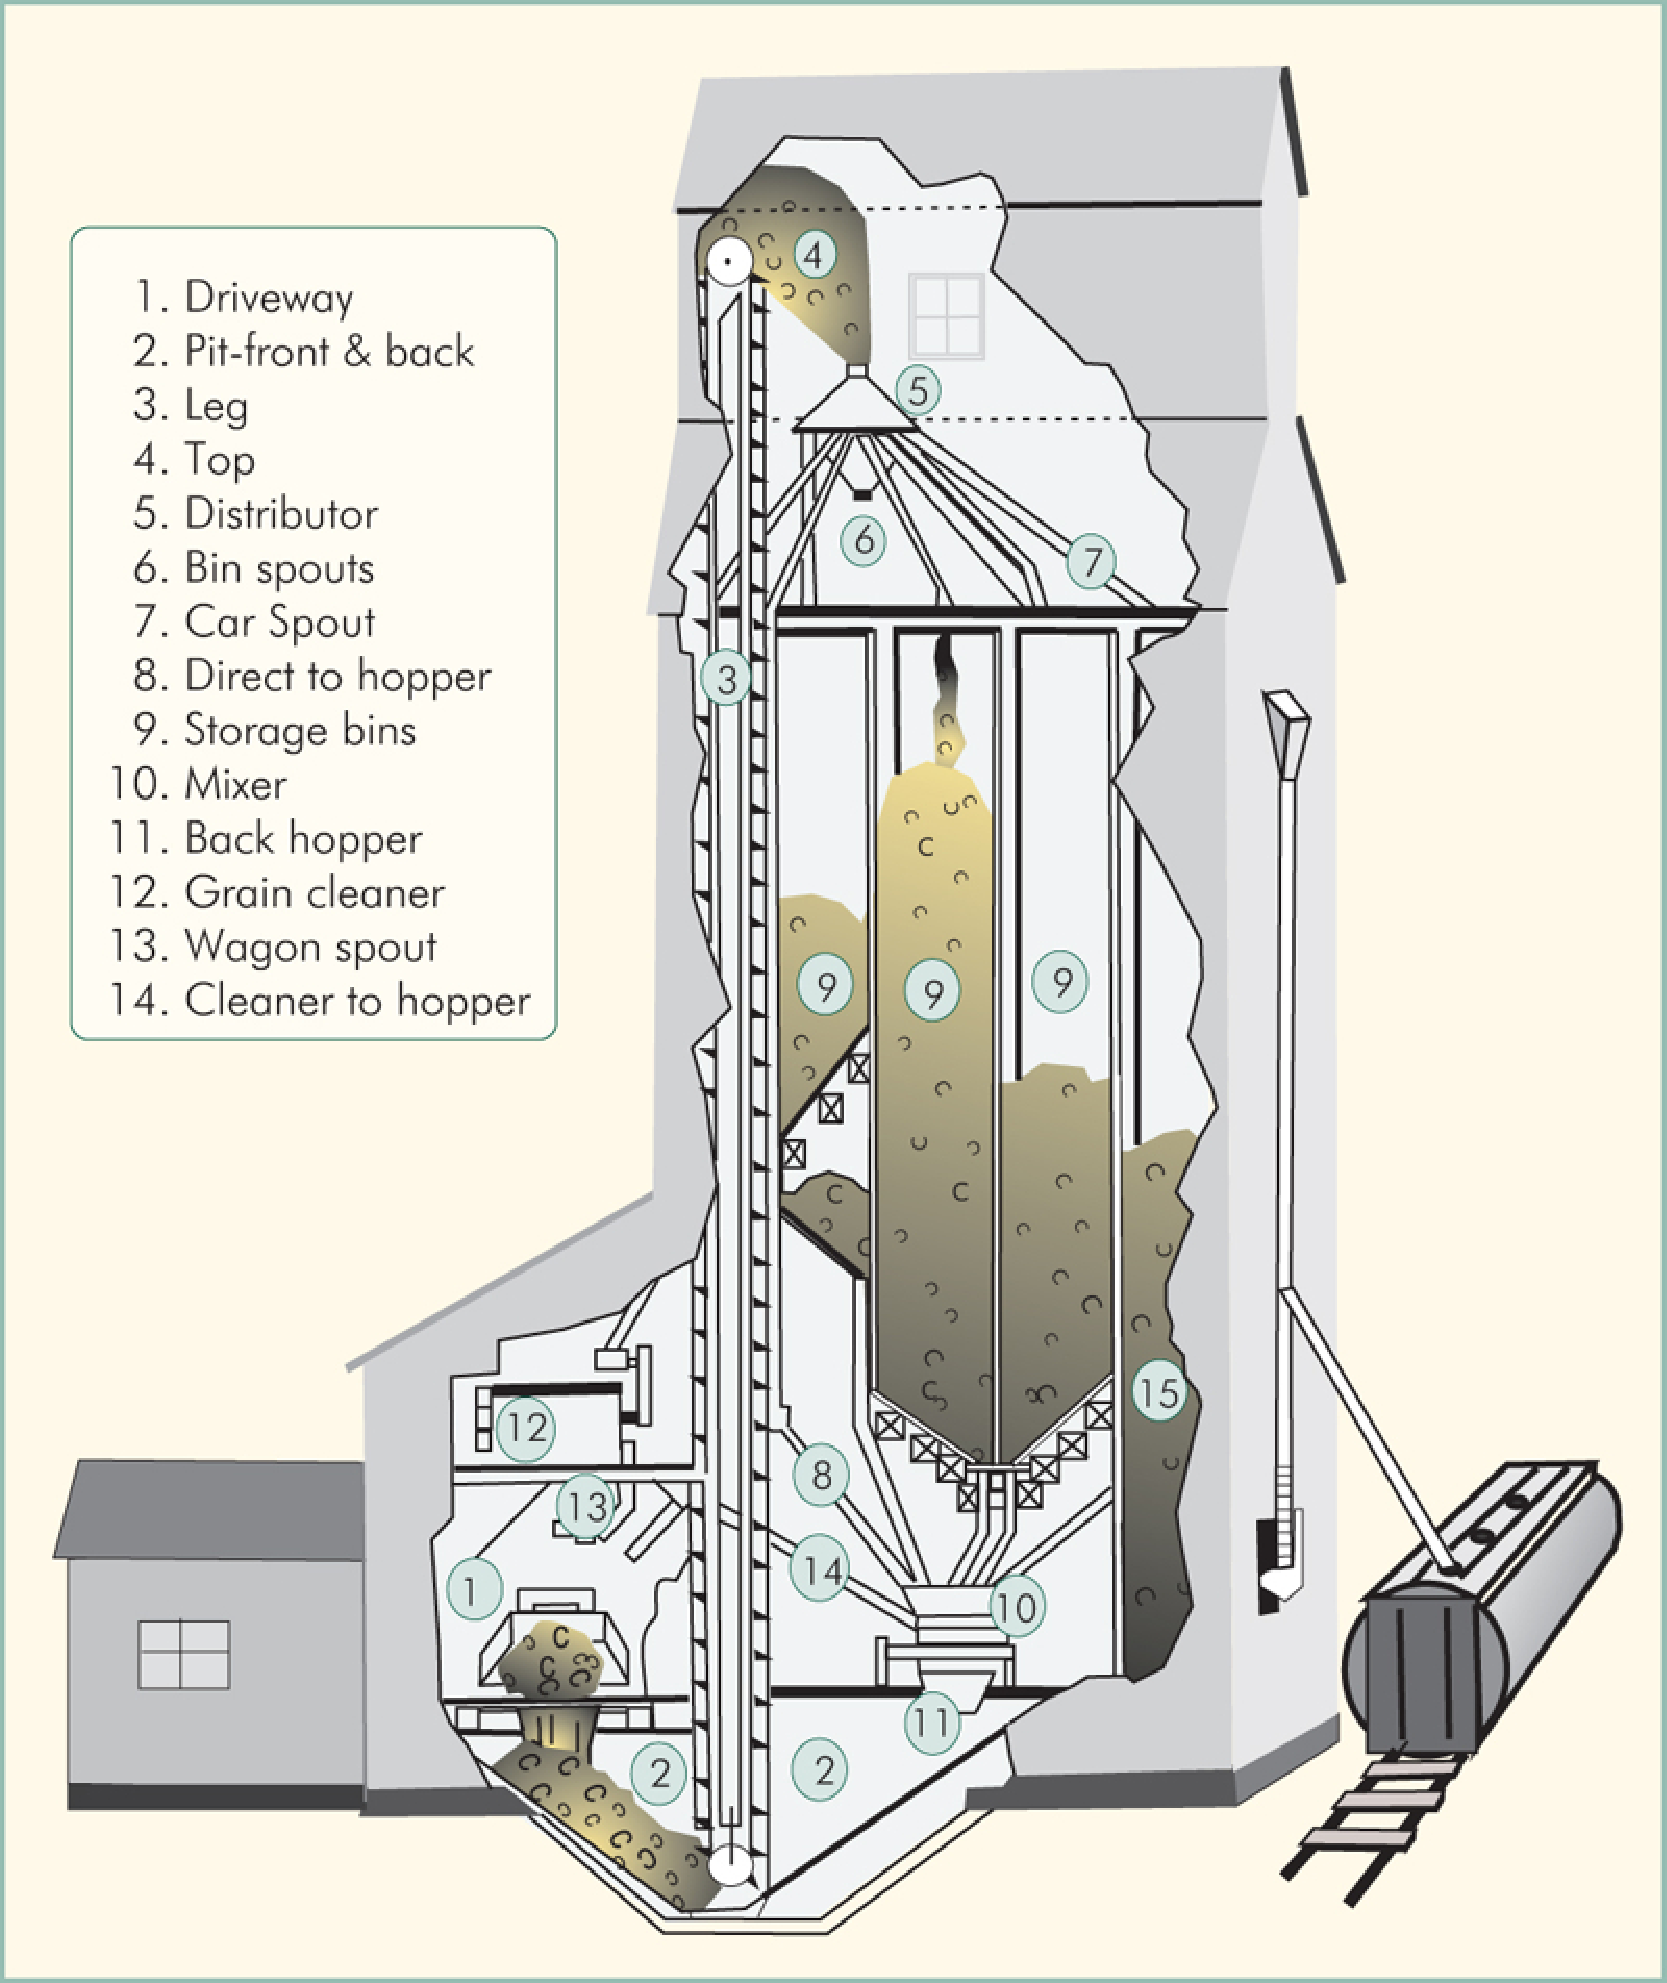
\includegraphics[width=0.8\linewidth]{./Appendix/grainleg.pdf}
    \caption{Cutaway of a Grain Elevator}\cite{grain_leg}
    \label{fig:grain}
\end{figure}

\noindent Gantry cranes are another option to move large amounts of material.  In the article "Unlocking the Power of Gantry Cranes: A Guide to Efficient Lifting," the author explains the features of a gantry crane\cite{maxim}.  Gantry cranes are designed to lift larger amounts of materials at once, rather than smaller amounts continuously.  A gantry crane consists of three main components: the structure, the trolley, and the hoist.  The structure provides the support for the crane, the trolley allows the lifted material to be moved laterally, and the hoist allows the material to be moved vertically.  The hoist is attached to the trolley, which is attached to the main beam of the structure. 
 Gantry cranes are commonly used in construction, manufacturing, and shipping.  Due to the high loads that tend to be experienced, gantry cranes are typically constructed out of steel; however, aluminum is sometimes used for parts that aren't as structurally strained.  The two main methods to power a gantry crane are to use either an electric or a hydraulic motor.\\




%%%%%%%%%%%%%%%%%%%%%



\begin{figure}[H]
    \begin{minipage}{0.5\linewidth}
        \centering
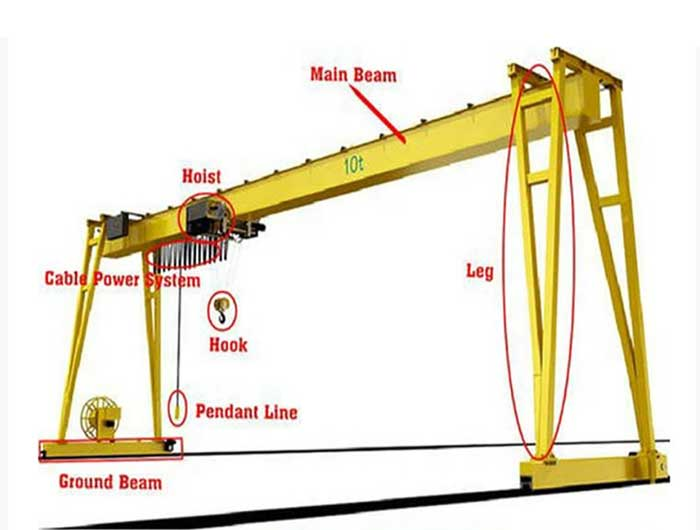
\includegraphics[width=0.6\linewidth]{./Images/Gantry/gantry.jpg}
    \caption{Gantry Crane}\cite{donqi}
    \label{fig:gantry}
    \end{minipage}%
    \hfill
    \begin{minipage}{0.45\linewidth}
        \centering
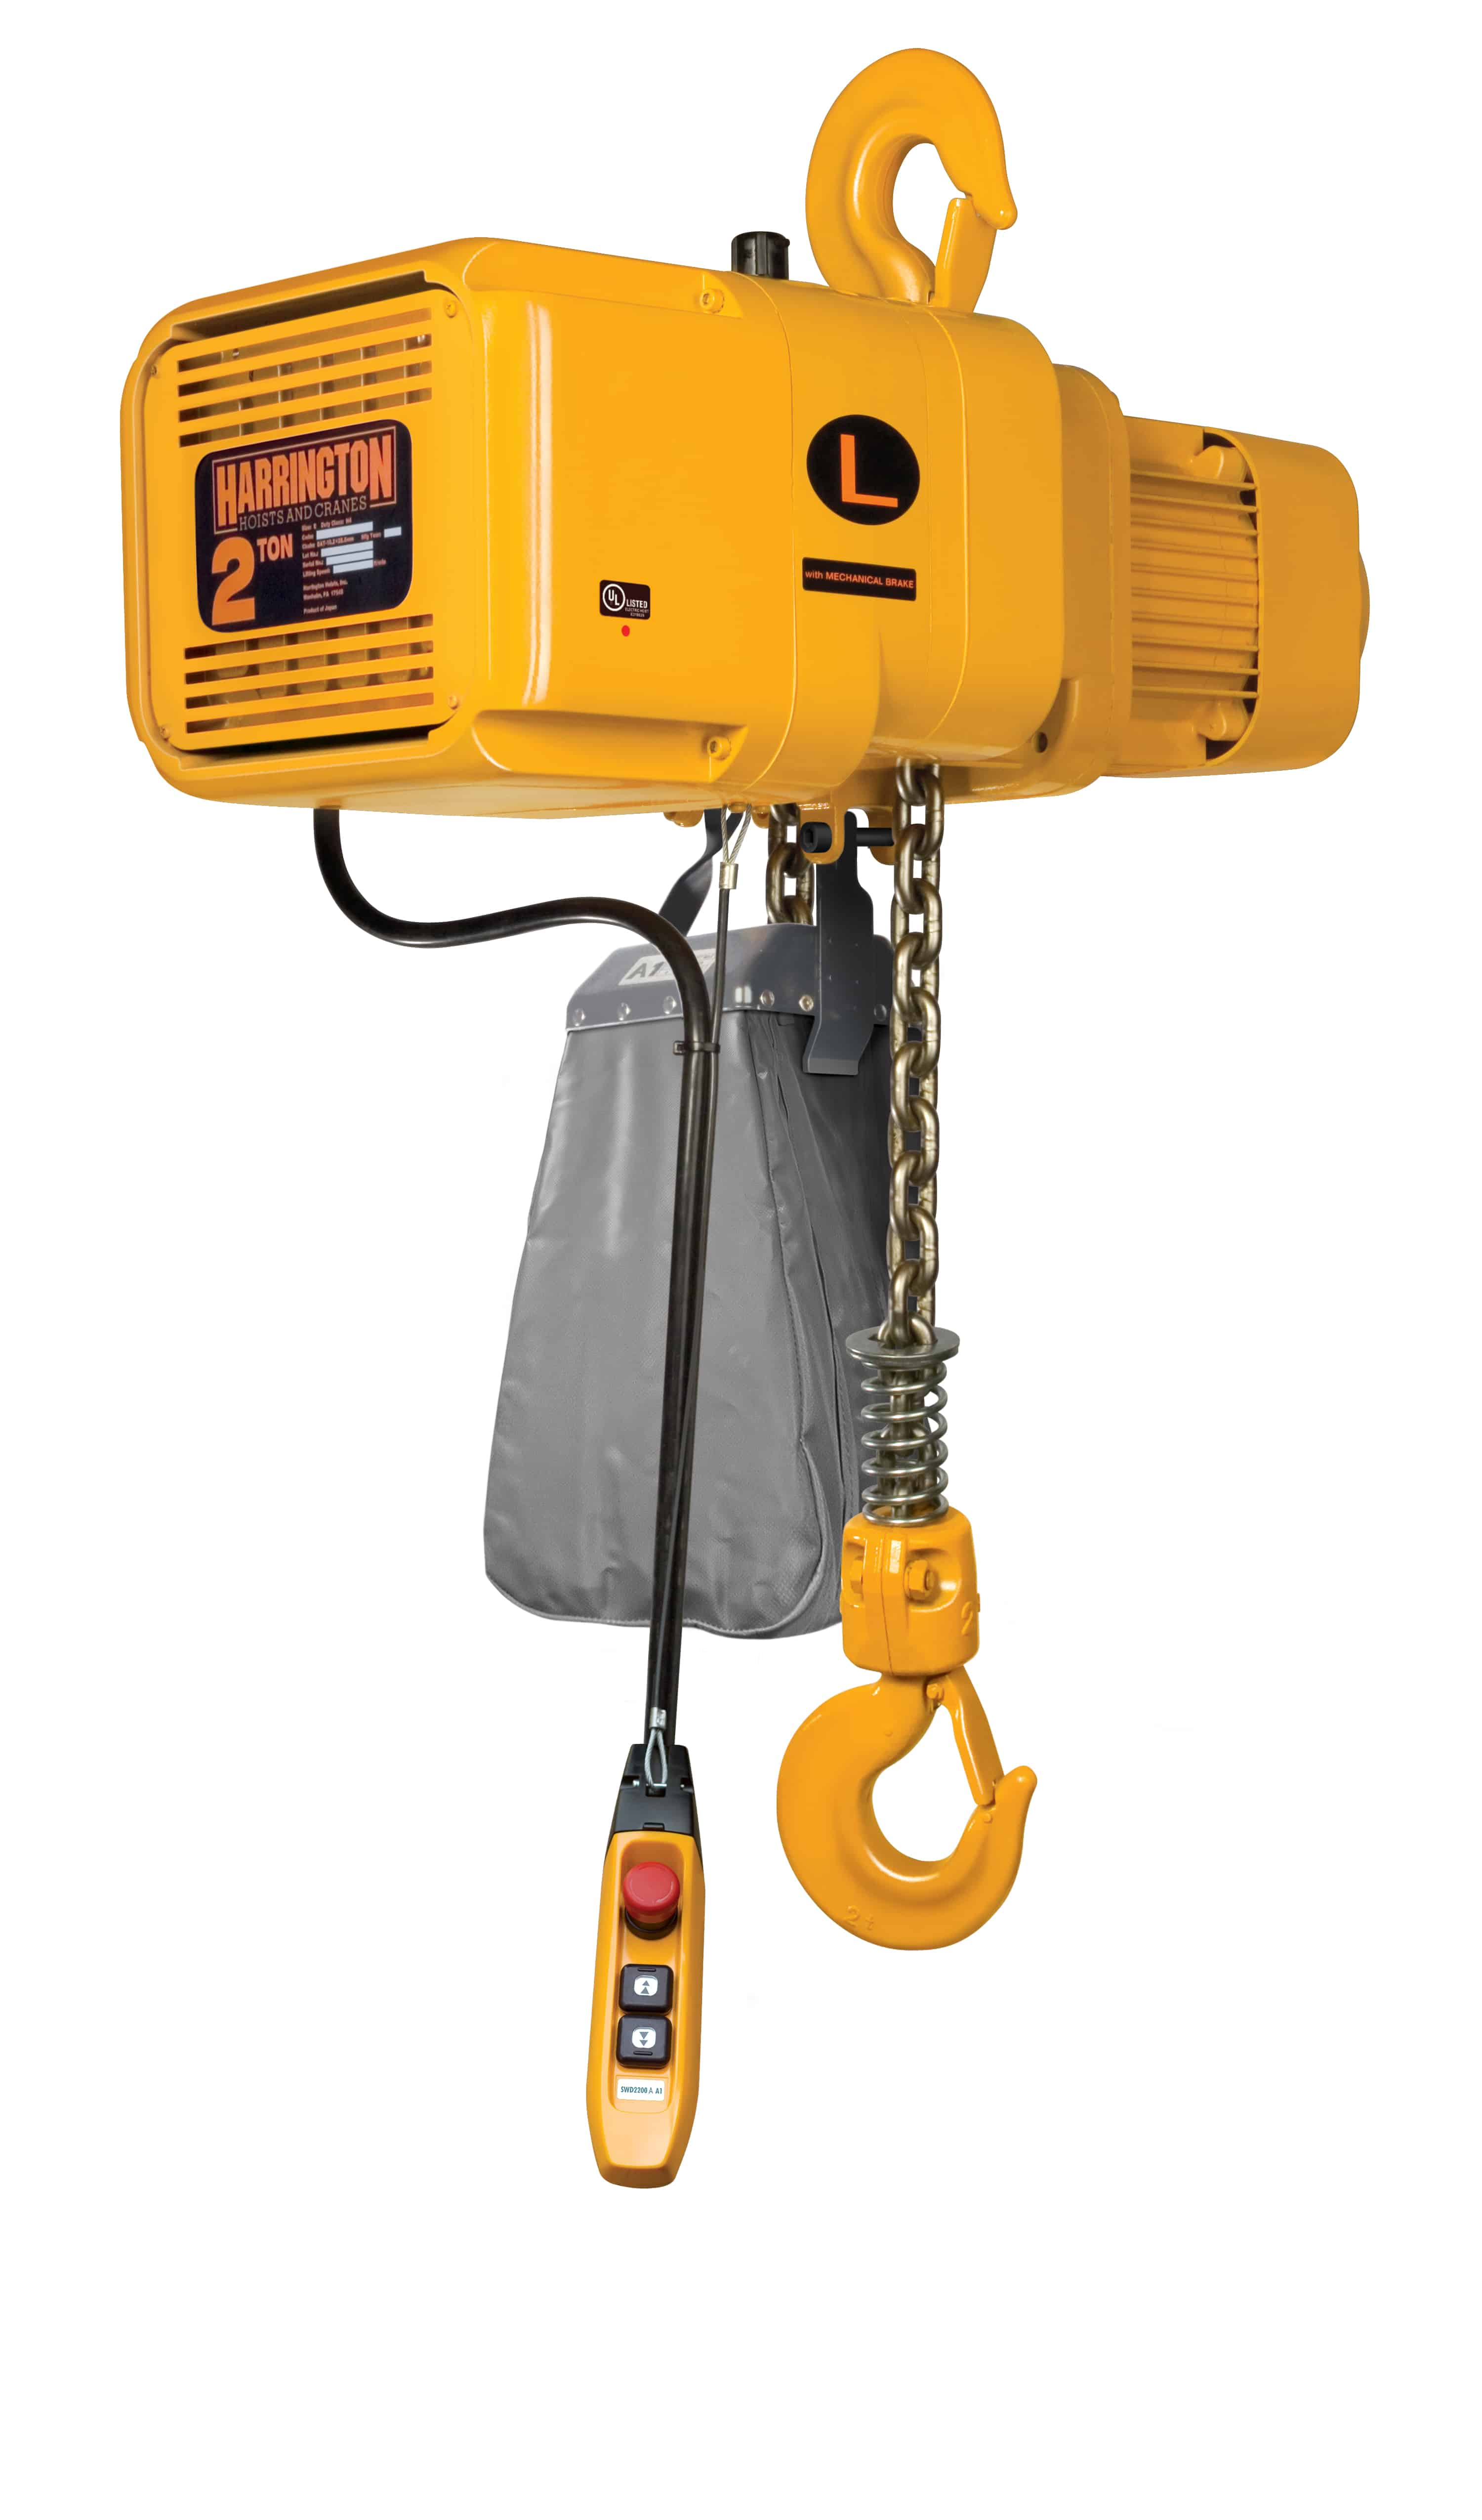
\includegraphics[width=0.6\linewidth]{./Images/Gantry/hoist.jpg}
    \caption{Gantry Crane Hoist}\cite{wallace}
    \label{fig:hoist}
    \end{minipage}
\end{figure}


%%%%%%%%%%%%%%%%%

\begin{figure}[H]
    \centering    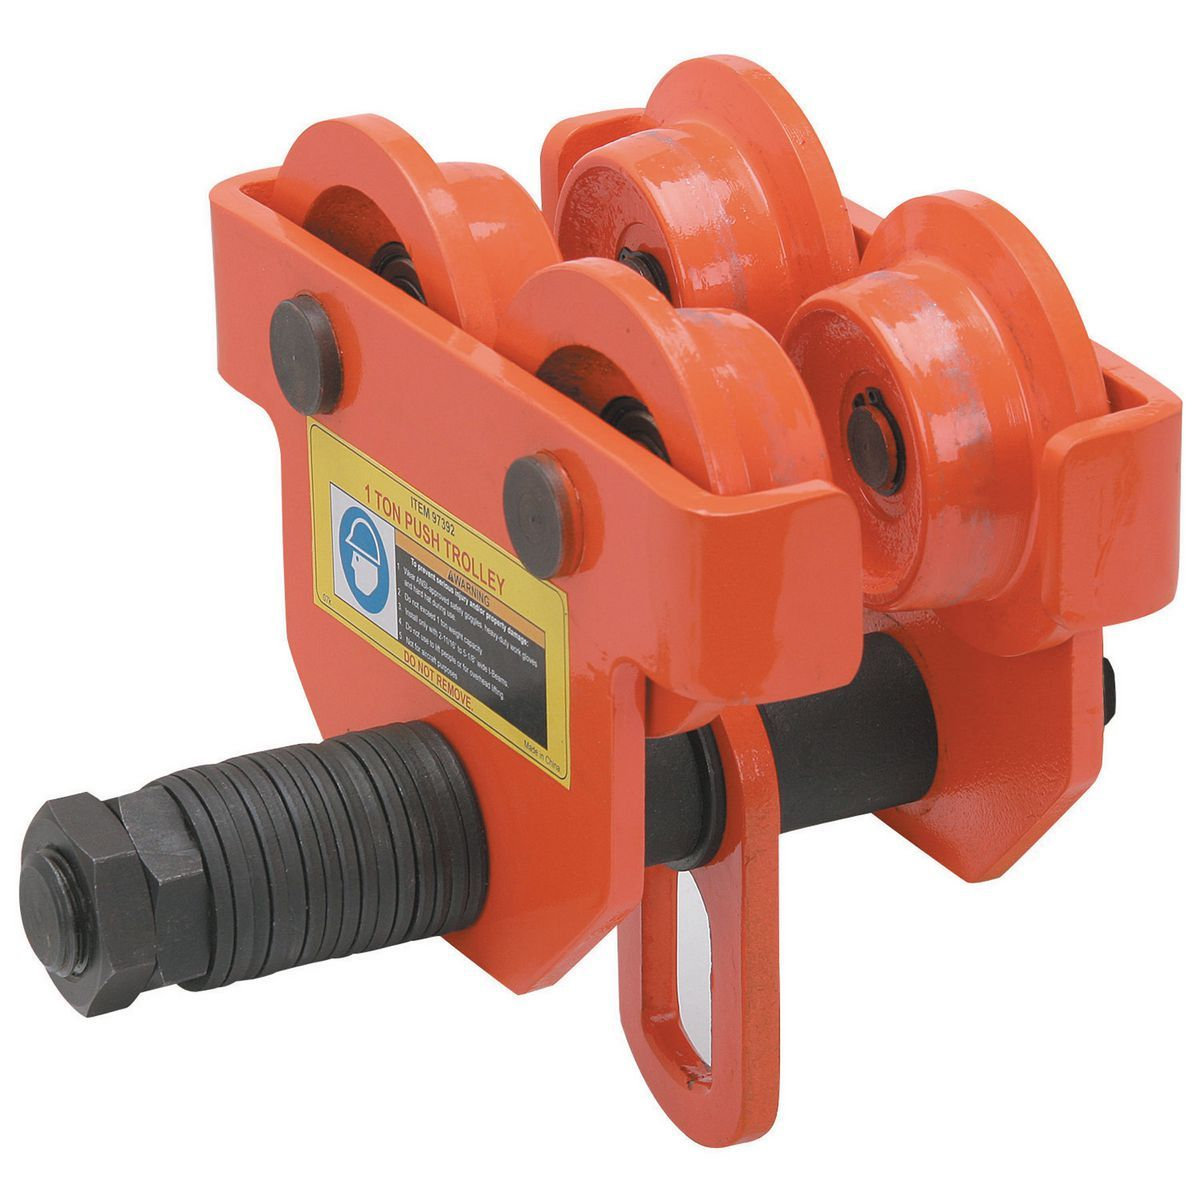
\includegraphics[width=0.3\linewidth]{./Images/Gantry/trolley.jpg}
    \caption{Gantry Crane Trolley}\cite{harbor}
    \label{fig:trolley}
\end{figure}

\noindent The last transportation method looked at for this project was a conveyor belt.  In the article "Belt Coveyors: Types, Components, and Applications," the author discusses the construction of belt conveyors and different variations that can be considered\cite{iqs}.  At a very basic level, a belt coveyor consists of a flexible belt stretched between multiple rollers that is driven by an electric motor.  There are five main components in a conveyor system: the head pulley, the tail pulley, idler rollers, the belt, and the frame.  The head pulley is attached to the drive motor, and is the component that transfers power from the motor to the belt.  It typically is the pulley with the largest diameter, and it is sometimes textured to improve traction between it and the belt.  The tail pulley sits on the opposite end of the conveyor belt.  It is sometimes adjustable to allow the system to be tensioned, but that can also be done with a separate device called a take-up roller.  Idler rollers are rollers along the path of the belt that are used to support and align the belt.  A variant of the basic idler roller of interest to this project is the troughing roller.  This device consists of three rollers arranged in such a way that it forcees the edges of the belt to curl inwards.  This type of conveyor is called a troughed belt conveyor\cite{conveyor}.  The main benefit of this conveyor belt variant is that it causes the material to track towards the center of the belt and thus reduces spillage of material.

\begin{figure}[H]
    \centering    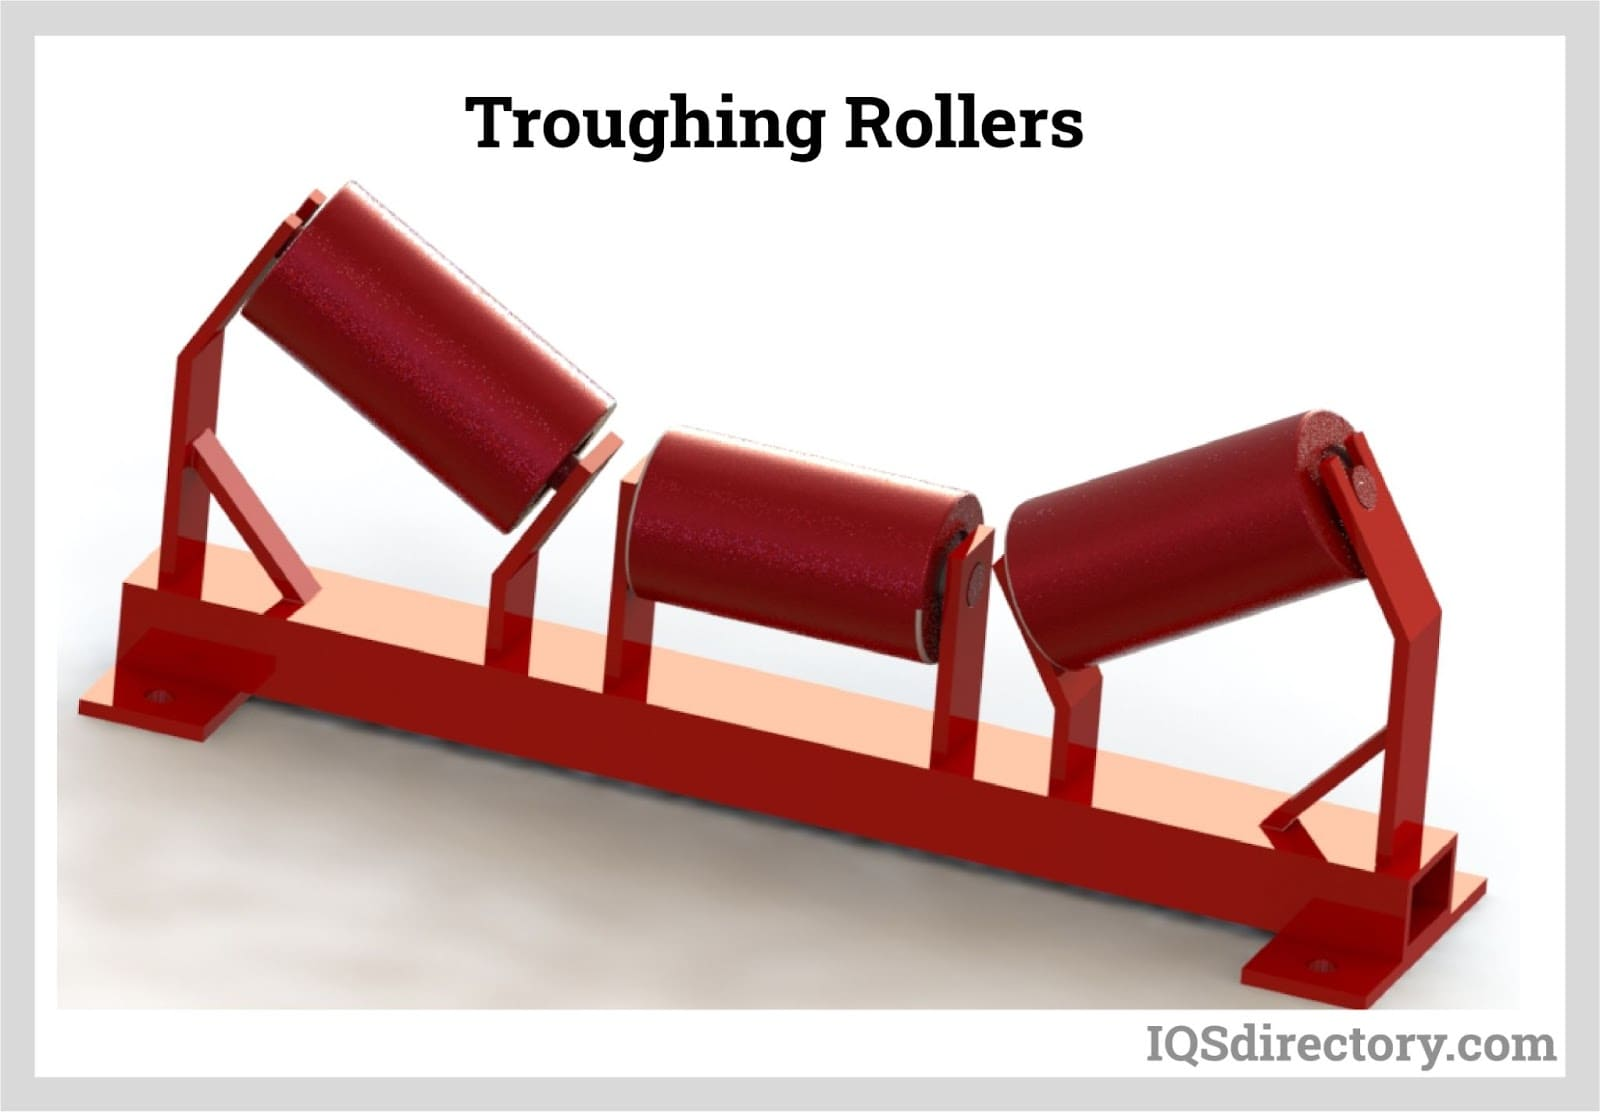
\includegraphics[width=0.5\linewidth]{./Images/Conveyor/troughing-rollers.jpg}
    \caption{Troughing Roller}\cite{iqs}
    \label{fig:troughing-roller}
\end{figure}

\noindent The belt is the part that interacts with the material being transported. 
 It is typically constructed of rubber or polymers, but other specialized materials can be used if needed.  The frame provides a mounting point for all the individual components of a conveyor belt.  Due to the variability of a conveyor system, the frame can take on many different appearances.  It is typically constructed out of steel, but aluminum extrusions can be used if the conveyor belt is not experiencing higher loads.\\\\
\noindent Due to the cold weather conditions of North Dakota, certain care must be taken when selecting the belt for a conveyor belt.  In the 2020 article "It's Cold Outside!  A Guide to Rubber Conveyor Belts Operating in Extreme Cold Conditions," Dr. Michiel Eijpe goes over the criteria that should be taken into consideration when selecting a belt for cold weather use\cite{marcel}.  When belts get too cold, belts tend to lose there elasticity, flexibility, and wear resistance.  If the belt gets too cold, it is even possible for the belt to become unable to even move around the pulleys. Eijpe says that due to the market for cold resistant conveyor belts being so small, specialized cold resistant belts aren't very common.  However, if the belt is of high-quality manufacture, abrasion resitant belts can be used, as they can usually withstand temperatures in the realm of -30 to -40 $\degree C$.  When selecting a cold-resistant belt, Dr. Eijpe gives three criteria:
\begin{enumerate}
    \item Ask supplier about their cold resistant testing methods.
    \item Have a minimum level of resistance to abrasion of less than 150 mm$^3$.
    \item Make sure that the belt is ozone and UV resistant.
\end{enumerate}



%Jonathan, WIP
%After getting onsite, it was determined that it is not necessary to lift the pellets to dump them into the neutralization pit.  Rather, because the pit is lower than the ground, the pellets can be transferred at grade before getting dumped into the pit.  Due to the corrosive environment, moving parts should be kept away from the pit so as to protect against corrosion and premature failure. Therefore, a passive system should be utilized for the final transfer into the pit.  

    

%  In an article put out by Feeco International\cite{conveyor}, several different types of conveyors are described.  The one most relevant to the project is the troughed belt conveyor, which consists of a rubber belt running over inclined steel rollers.  The rollers cause the belt to dip in the middle, causing the material to track towards the center and prevents it from falling off the sides.

\begin{figure}[H]
    \centering
    
\includegraphics[width=0.5\linewidth]{Senior Design Project Template//Figures/Troughed-Belt-Conveyors.jpg}
    \caption{Troughed Belt Conveyor\cite{conveyor}}
    \label{fig:TroughedBelt}
\end{figure}


\subsubsection{Electrical Specifications} \label{sec:elecspec}%Ben - thinking like code requirements and what needs to be looked at. Electrical equipment and its use in refinery areas

The electrical equipment in this project will be installed in a Class 1 Division II zone. This designation requires that all electrical equipment complies with the specifications set forth in the National Electrical Code (NEC). In the article, \textit{Class and Division: Don't Break Rank on Your Next Installation.}, Mike Holt discusses the proper standards established by the NEC.\cite{Class and Division} Holt explains that Class 1 Division II is governed by Articles 500 and 501 of the NEC, providing a detailed explanation of these codes. The most relevant codes for the project include those related to motors, enclosures, surge protection, and wiring methods. Motors must be explosion-proof enclosed motors as specified in NEC 501.125(B). The enclosures for Class I, Division I, and Division II are identical. Enclosures and connectors must utilize explosion-proof cords as outlined in NEC 501.10.3. Surge protectors may be installed inside the enclosures, according to NEC 501.35. For wiring methods, Mike recommends using cables such as MI, MC, MV, or TC with termination fittings, in compliance with NEC 501.10(B). The project will be constructed in accordance with all NEC code requirements.

\subsection{Product Specifications} % Gannon - Done

This section outlines the measurable criteria for the project, ensuring feasibility, performance, and compliance with applicable industry standards. 

\begin{table}[htbp]
\centering
\caption{Design Specifications}
\begin{tabular}{|p{0.15\textwidth}|p{0.75\textwidth}|}
\hline
\textbf{Category} & \textbf{Specifications} \\
\hline
\hline
Electrical & All electrical equipment must conform to class 1 division 2 specifications. \\
\hline
Electrical & All electrical equipment must abide by the National Electric Code (NEC) standards. \\
\hline
Safety & The design must include fail-safe mechanisms such as emergency stops, load indicators, and anti-slip platforms. \\
\hline
Performance & The lift mechanism shall transport the calcium chloride pellets to the neutralization pit faster than the neutralization pit consumes them. \\
\hline
Operation & The mechanism should allow for a single operator to use without the need for additional personnel. \\
\hline
Materials & All components in contact with CaCl$_2$ must be constructed from coated A36 steel to withstand prolonged exposure. \\
\hline
Space & All systems shall be designed within the designated space surrounding the Bulk Bag Unloader. \\
\hline
\end{tabular}
\end{table}



\subsection{Additional Considerations} % Gannon
This section outlines any additional considerations when designing that may not have directly measurable criteria as compared to the previous section. 

\begin{itemize}[noitemsep, topsep=0pt]
    \item The lift mechanism shall safely transport the calcium chloride pellets to the neutralization pit, keeping any operators out of harm's way. 
    \item All systems shall allow for easy accessibility and ease of repair if needed.
    \item Weather: All systems shall be designed with harsh North Dakota weather in mind.
\end{itemize}


\subsection{Requirements Traceability Matrix} % Ben

The Requirement Traceability Matrix is a vital component of this project. It ensures that the project meets the standards established by the design team, the company, and other regulatory authorities. Marathon needed a design to transport calcium chloride to a neutralization pit. The design will be installed in a Class I Division II zone, so all components must adhere to the safety standards established for these areas. The engineering team was given flexibility in the design process, with safety being the top priority. 

\begin{figure}[H]
    \centering
    
\includegraphics[width=1\linewidth]{Senior Design Project Template//Figures/traciblity_matrix.png}
    \caption{Requirement and traceability matrix}
    \label{fig:Requirements&TracabilityMatrix}
\end{figure}


\section{Product Design}
%\vspace{-0.8cm}
%Describes the technical design of the solution to the engineering problem, including the identification of systems and subsystems, and interfaces between subsystems. All specifications shall be assigned to the system, one or more of the subsystems and/or interfaces and a brief explanation of how each of the specifications is satisfied. This process ensures that all specifications are addressed in the design and verified an appropriate manner. 

%This section is a significant part of the outcomes of your project because this is the documentation that communicates to others what your design is.  The structure of this section should reflect the structure of your design project. You will first want to describe the overall design project and all its parts (for instance the various subsystems of a quadcopter). You will then dedicate subsections to each of those parts. This section will reference Appendices where design documents (like drawing packets and bills of materials, or construction plans) will appear to go into highly specific technical details of the design.  



\subsection{Mechanical Design} \label{sec:mechDes}
%needs to be updated
%\vspace{-0.7cm}
The design that was chosen for this project was a conveyor belt.  This design consists of two subsystems.  The first subsystem is an unloading system.  This subsystem accepts the calcium chloride bags and facilitates the unloading and transfer of the $CaCl_2$ to the conveyor belt.  The second subsystem is the conveyor system.  This system will take the pellets from the unloading system and transport them to the neutralization pit.  For all subsystems, special care will be taken to protect the pellets from the environment, as well as to provide access ports to allow for cleaning when the system becomes clogged by the calcium chloride.\\

\begin{figure}[H]
    \centering
    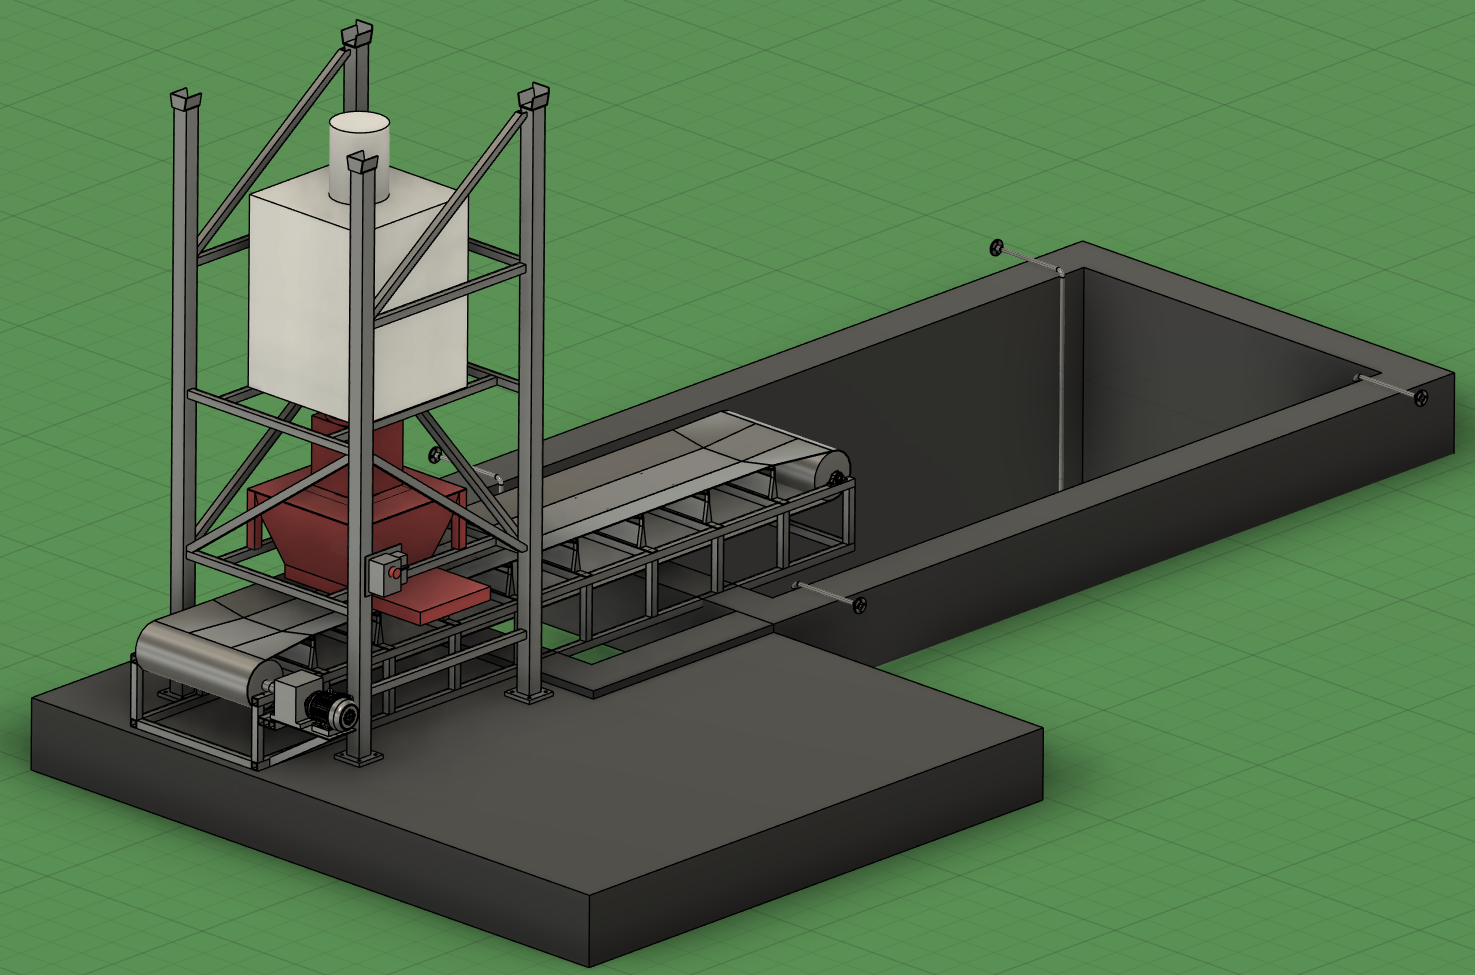
\includegraphics[width=0.7\linewidth]{./Images/proposed.png}
    \caption{Model of Proposed System}
    \label{fig:proposed}
\end{figure}

\subsubsection{Bulk Bag}\label{sec:bulkbag}
%\vspace{-0.7cm}
The bags that will be used to transport the $CaCl_2$ are FIBC bags from Sun Coast Packaging, LLC\cite{Marathon}.  These bags are composed of a 4-foot tall, 3 foot square center component, with cylindrical 14 inch diameter inlet and outlet sections that are both 18 inches tall, as shown in Figure \ref{fig:bulkbag}.  This gives the bag a total height of 7 feet.  Four 10-inch long loops are attached to the top to provide an attachment point to lift the bag.  The datasheet for this bag can be found in Section \ref{sec:bulk}.
\begin{figure}[H]
    \centering
    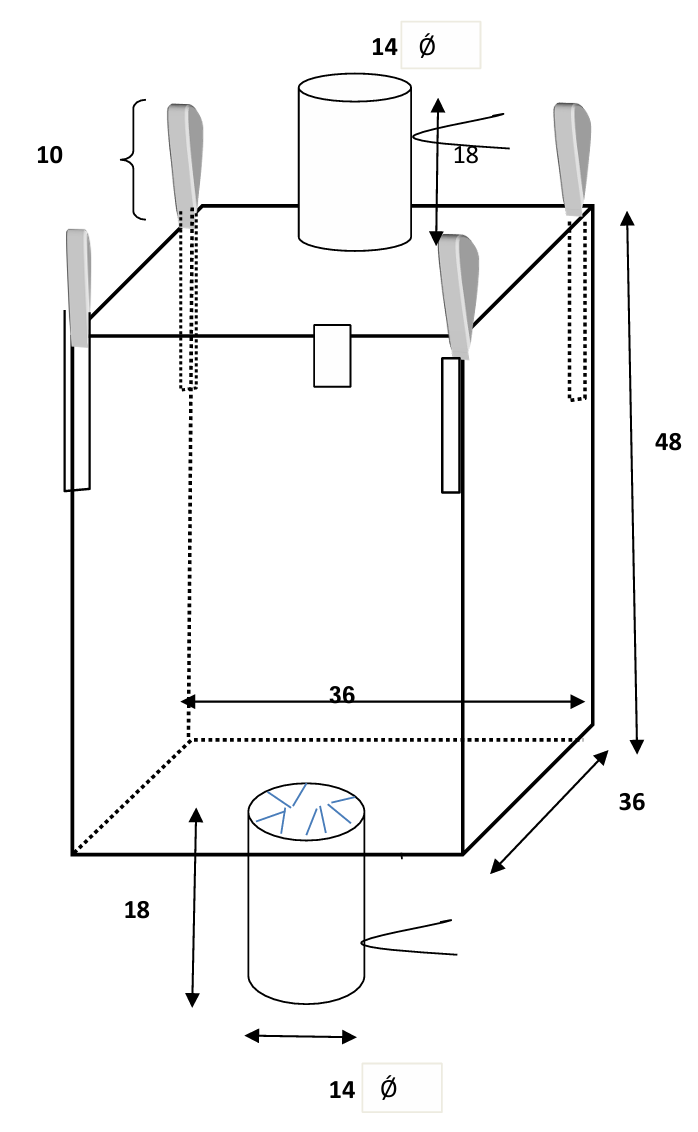
\includegraphics[width=0.5\linewidth]{./Images/Bulk Bag/bulkbag.png}
    \caption{Engineering Drawing for the Bulk Bag that will be used}
    \label{fig:bulkbag}
\end{figure}
\subsubsection{Unloading System}\label{sec:UnloadingSystem} %Jonathan

The unloading system is constructed of A500 Grade B steel tubing.  For the upright support beams, 4"x4"x1/4" tubing was used.  To guarentee that these beams will not fail under normal use cases, these beams were analyzed under several failure methods.  First, failure under bending was analyzed using the equation $$\sigma_b = \frac{Mc}{I}$$
with:\\
$\sigma_b$ = the bending stress
$M$ = the bending moment experienced, equal to the force times the length\\
$c$ = the distance from the center of the tube to the outside edge\\
$I$ = the area moment of inertia of the tube\\\\
The force being applied is assumed to be evenly distributed across each of the supports.  Since there are four upright supports, each support will be experiencing 500 lbs of force.  With a height of 150 inches, this gives the experienced bending moment as $M = 75,000$lb-in.  Since this is a 4 inch wide square tube, $c$ is equal to 2 inches.  $I$ can be found using the equation $$I = \frac{WH^3-wh^3}{12}$$

\noindent with:\\
$W$ = the outside width\\
$H$ = the outside height\\
$w$ = the inside width\\
$h$ = the inside height\\\\
Since the cross section is a square, $W$ equals $H$ and $w$ equals $h$.  The outside dimensions are known as 4 inches, and the inside dimensions can be found by subtracting two times the wall thickness, resulting in an inside width of 3.5 inches.  Solving for this equation, $I$ is found to equal 8.828 in$^4$.\\
Solving now for the equation, the bending stress experienced by the support is shown to be $\sigma_b = 16,991.39$psi.  A500 Grade B steel has a yielding strength of 46,000 psi\cite{a500}, which means this support has a safety factor of 2.71.\\\\
The next failure mode that was analyzed was for axial stress.  This was accomplished using the equation $$\sigma = \frac{F}{A}$$
where $\sigma$ is the axial stress experienced, $F$ is the axial force experienced and $A$ is the cross sectional area.  Since the force will also be assumed to be evenly distributed here, $F$ is known to equal 500 lbs.  $A$ can be found by subtracting the area of the inside dimensions form the area of the outside dimensions.  By doing this, $A$ is found to equal 3.75 in$^2$.  Solving the equation, $\sigma$ is found to equal 133.33 psi.  This means that there is a safety factor of 345 for failure in the axial direction.\\\\
The last failure mode that was investigated was buckling.  The equation used to find the force required for buckling was $$F = \frac{n\pi ^2EI}{L^2}$$
where $n$ equals the end condition factor, $E$ equals the Young's Modulus, $I$ equals the area moment of inertia, and $L$ equals the length of the tube.  Since this tube can be modeled as a beam with one end fixed and one end free, $n$ can be set equal to 0.25\cite{buckling}.  The Young's Modulus of A500 Grade B steel is 29,000,000 psi\cite{a500}.  $I$ has been calculated previously as being 8.828 in$^4$, and L is 150 inches.  Using these values, $F$ can be found to be equal to 28,075 lbs.  Since each beam will only experience 500 lbs, this gives a safety factor of 56.15 against buckling.\\\\
In addition to these calculations, a Finite Element Analysis of the structure was conducted inside of Fusion for both axial loading and bending.  The results provided by the FEA align with the calculated values.\\\\

\vspace{0.2cm}

\begin{figure}[h]
    \begin{minipage}{0.45\linewidth}
        \centering
        
        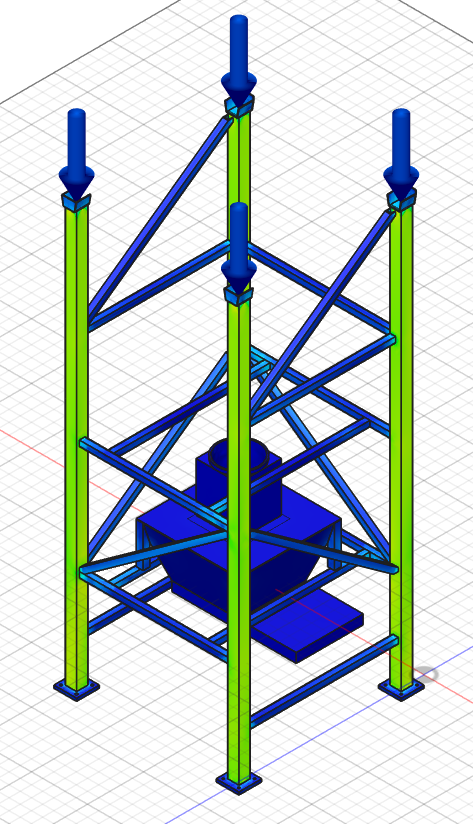
\includegraphics[width=0.8\linewidth]{./Images/FEA/axial.png}
        \caption{\label{img:axial}Finite Element Analysis for Axial Stress}
        
    \end{minipage}
    \hfill
    \begin{minipage}{0.45\linewidth}
         \centering

        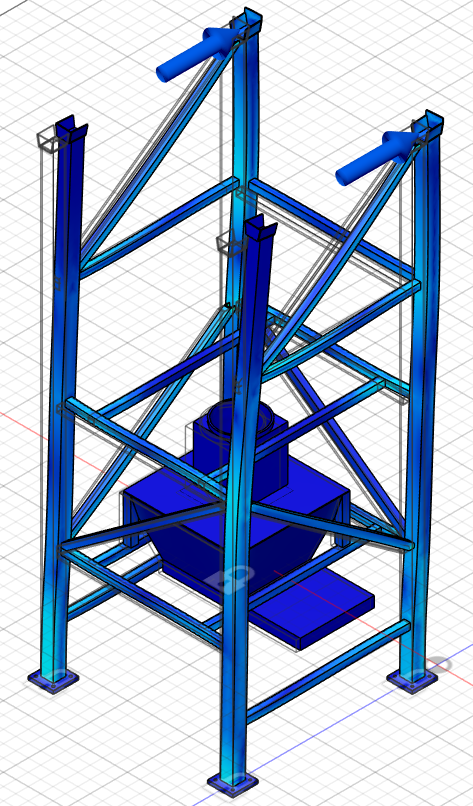
\includegraphics[width=0.8\linewidth]{./Images/FEA/bending.png}
        \caption{\label{img:bending}Finite Element Analysis for Bending Stress}
    \end{minipage}
\end{figure}
\newpage

\noindent For the rest of the structural tubing, 2"x2"x1/4" tubing was used.  This is mainly used to support the slide valve, hopper, and cutter mechanisms, as well as provide bracing for the upright supports.  Since it will be supporting significantly less weight than the upright supports, it did not have to withstand as much load, and thus a smaller cross section was able to be used.  The base plates that are bolted into the concrete pad are constructed of 1" thick A36 steel plate, and the caps that are used to align the lifting mechanism for the bag are constructed out of 1/4" A36 steel plate.  The engineering drawings for this can be seen in Section \ref{sec:drawing}\\\\
The final dimensions for the Unloading Structure came out to be 12 feet 7.5 inches tall, 5 feet 5 inches wide, and 5 feet 5 inches deep.  These values can be seen in Figure \ref{fig:dimensions}.\\\\
Because of the decision to reuse part of the current structure, a demolition plan was needed to be provided to explain what parts are to be kept and which parts were to be demolished.  This plan can be found in Section \ref{sec:demolish}.

\begin{figure}[H]
    \centering
    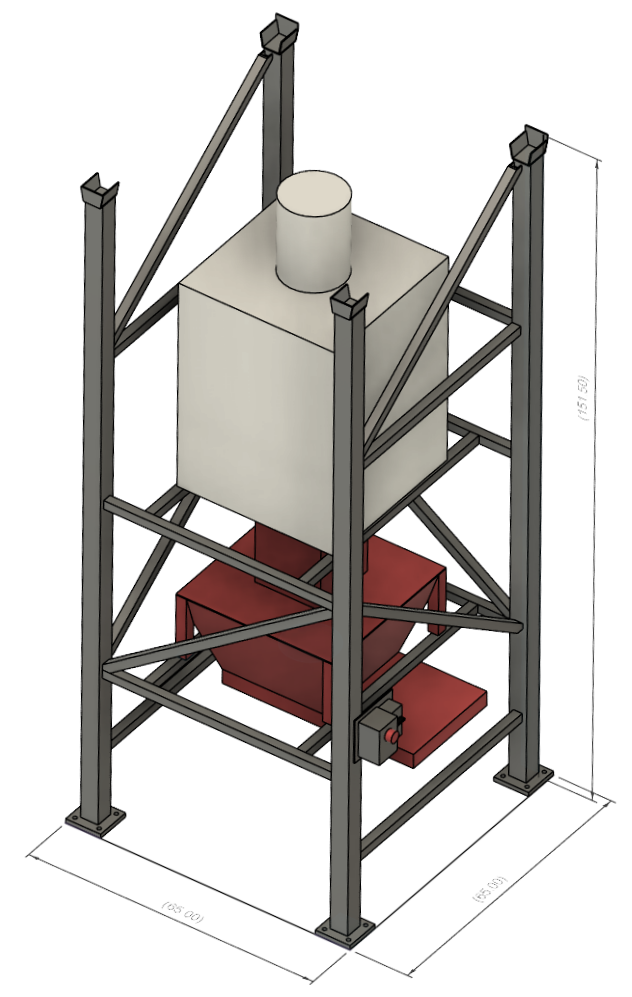
\includegraphics[width=0.5\linewidth]{./Images/Structure/dimensions2.png}
    \caption{New Design for Unloading Mechanism (Gray) with Reused Components (Red) and Bulk Bag Attached (White).  }
    \label{fig:dimensions}
\end{figure}

%\vspace*{-1cm}
\subsubsection{Conveyor System} \label{sec:ConveyorSystem} %Jonathan

The conveyor system utilized for this project follows a troughed belt design.  At one end pellets will be deposited onto the belt from the unloading mechanism.  At the other end, the belt will unload the pellets directly into the neutralization pit.  The exact specifications for the belt used can be found in Section \ref{pdf:belt}.  The system uses a three foot wide belt with a trough angle of 10\degree.  It was decided to construct the frame out of the same 2"x2"x1/4" A500 Grade B steel tubing that the Unloading Structure uses.  The main purpose of this was to minimize the number of unique parts needed.    The engineering drawings for this can be found in Section \ref{pdf:conveyor}.

\begin{figure}[H]
    \centering
    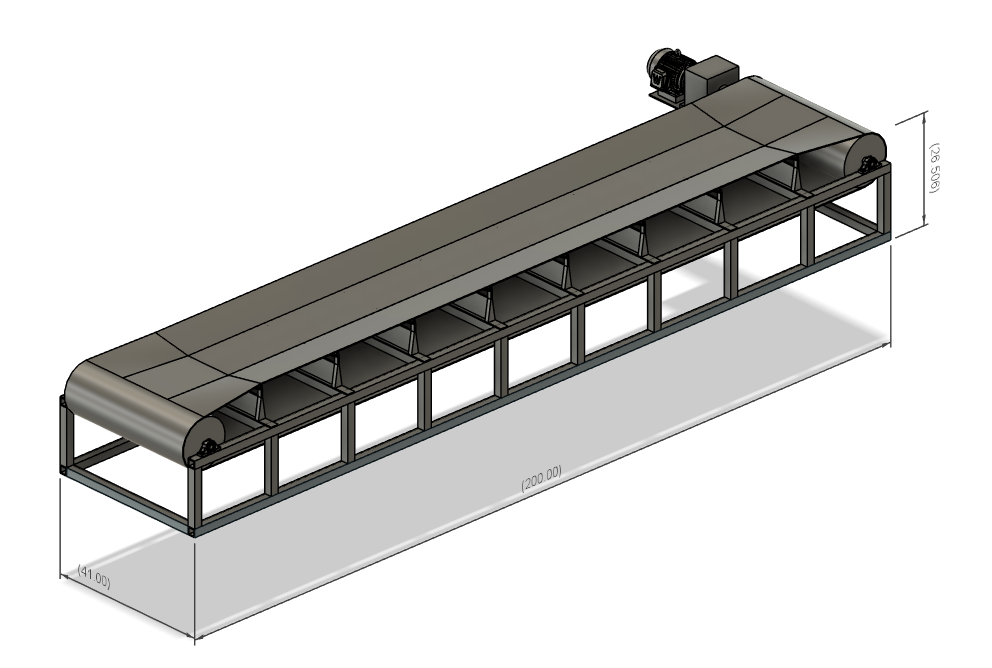
\includegraphics[width=0.6\linewidth]{./Images/Conveyor/ConveyorBeltAssembly.png}
    \caption{Conveyor Belt Assembly}
    \label{fig:ConveyorBeltAssembly}
\end{figure}
\begin{figure}[H]
    \centering
    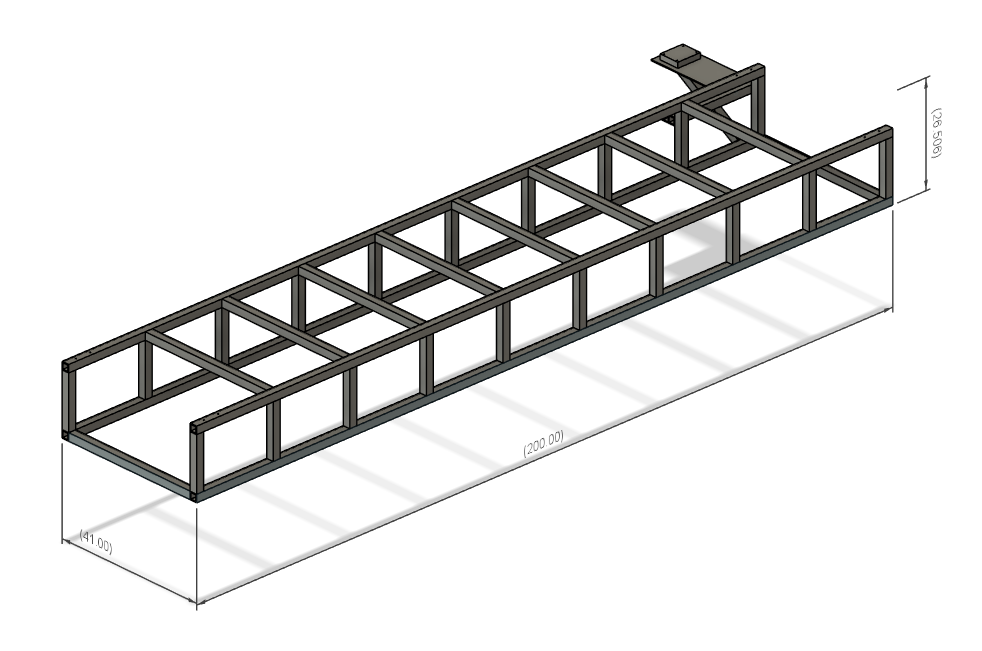
\includegraphics[width=0.6\linewidth]{./Images/Conveyor/ConveyorFrameAssembly.png}
        \caption{Frame Section}
        \label{fig:ConveyorFrame}
\end{figure}
\begin{figure}[H]
        \centering
        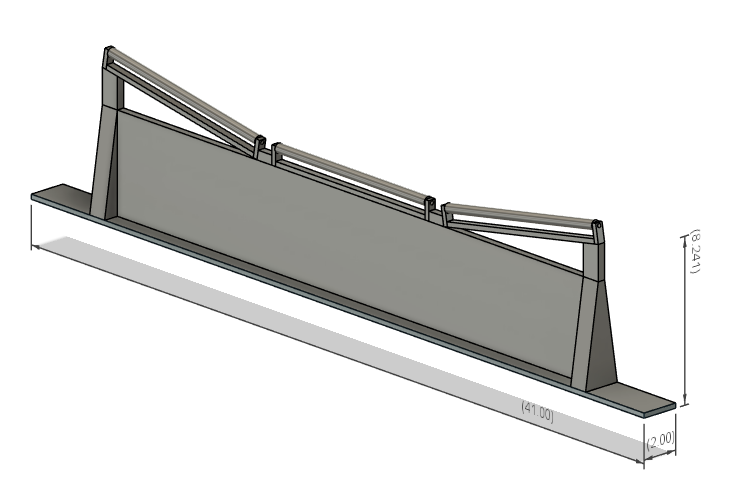
\includegraphics[width=0.6\linewidth]{./Images/Conveyor/TroughedIdler-Final.png}
        \caption{Troughing Roller}
        \label{fig:TroughedIdler}
\end{figure}

\subsubsection{Mixer}
\label{sec:MixingSystem} %Jonathan

The mixer consists of four 3/4" air lances located at each corner of the neutralization pit.  At the base of each lance, the pipe transitions 90$\degree$ into a horizontal section.  Each of the horizontal sections is welded at an angle to the downpipe so that air is directed from four directions to the point where the pellets drop.  These 4 streams serve to create a region of turbulent flow and circulating currents that will serve to dissolve the pellets faster.  At the top of each lance, the existing pipe will be cut and a flange will be welded in.  This will allow for an easy replacement of the lance when it corrodes.  Since air will now exit the pipe at a 90$\degree$ angle, the bending moment created by this must be considered.  At Marathon's request, the lances will be set in the corners of the pit and braced against its walls.  The walls will then provide a reaction force and prevent any flexing.  They do not expect any increased wear on the walls of the pit from the lances, but if any is observed, pipe shoes will be fitted to the lances to solve that issue.  The engineering drawings for this system can be found in Section \ref{pdf:mixer}.
\begin{figure}[H]
    \begin{minipage}{0.45\linewidth}
        \centering
        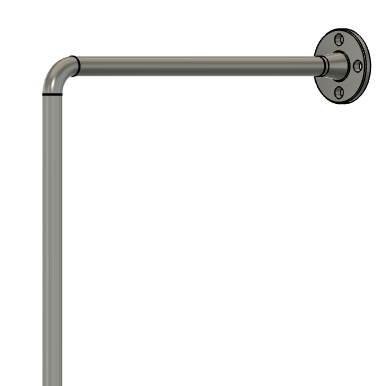
\includegraphics[width=0.8\linewidth]{./Images/Mixer/MixerFlange.png}
        \caption{Flange to Downpipe Section}
        \label{fig:MixerFlange}
    \end{minipage}%
    \hfill
    \begin{minipage}{0.45\linewidth}
        \centering
        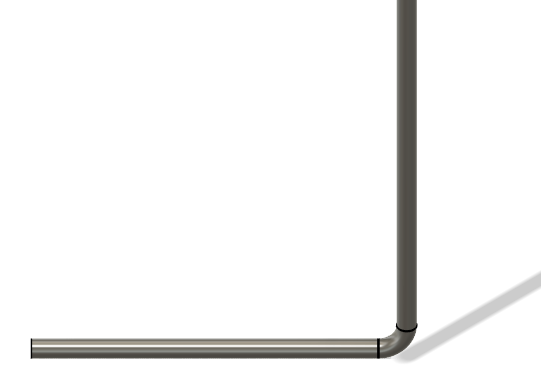
\includegraphics[width=0.8\linewidth]{./Images/Mixer/MixerBottom.png}
        \caption{Downpipe to Horizontal Section}
        \label{fig:MixerBottom}
    \end{minipage}
\end{figure}
\begin{figure}[H]
       \centering
       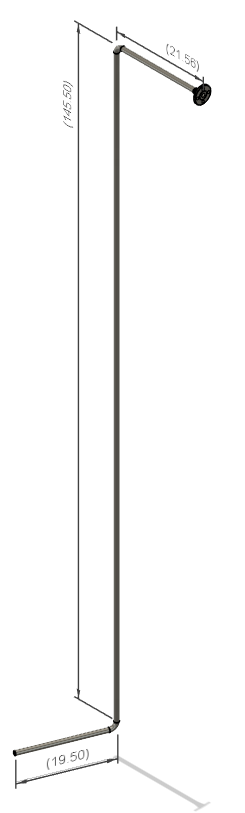
\includegraphics[width=0.35\linewidth]{./Images/Mixer/MixerAssembly-Final.png}
        \caption{Complete Mixer Assembly}
        \label{fig:MixerFull}
\end{figure}
\begin{figure}[H]
        \centering
        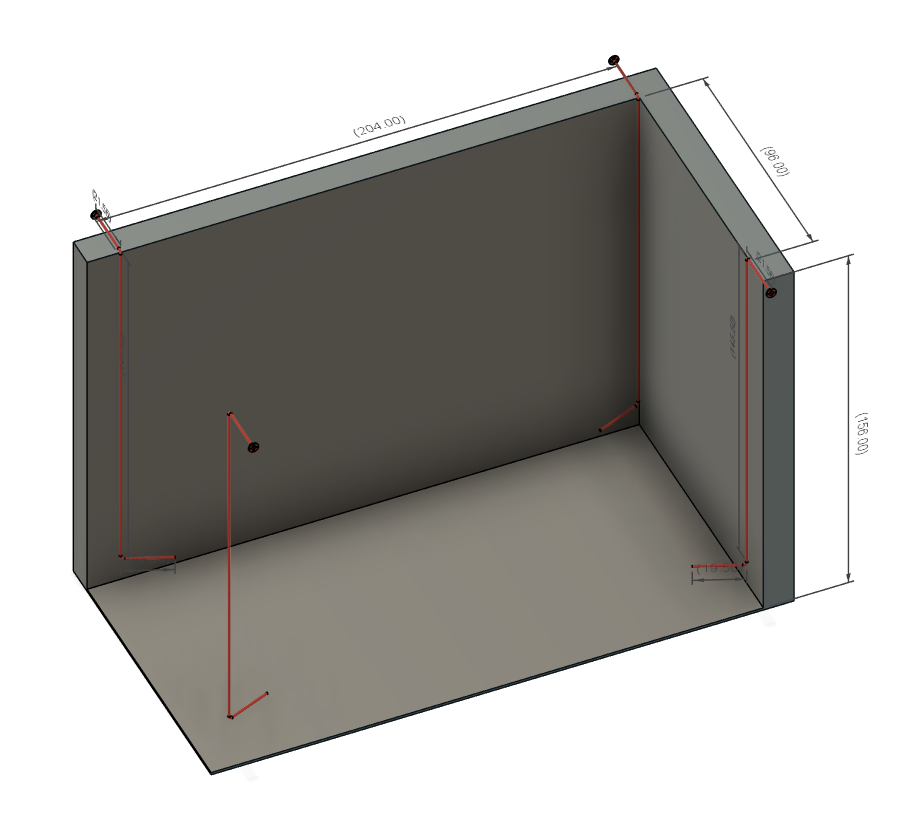
\includegraphics[width=0.8\linewidth]{./Images/Mixer/FullMixerInPit.png}
        \caption{Cutaway View of All Four Air Lances in the Neutralization Pit}
        \label{fig:MixerOverhead}
\end{figure}

\subsection{Mechanical Bill of Materials}\label{sec:mechbom}

\begin{center}
\begin{tabular}{|l|l|l|l|l|}

\hline
Item & Description & Quantity & Link to Website & Cost \\
\hline
\hline
VASM-SXXW-X & 18" Square manual roller gate valve  & 1 & Flexicon & Already on site \\
\hline
CVD-S36 & Hopper cover & 1 & Flexicon & Already on site \\
\hline
 HPX1-S36-X & Hopper & 1 & Flexicon & Already on site \\
\hline
 IVM-12 & 12 inch diameter iris valve & 1 & Flexicon & Already on site \\
\hline
 4"x4" Steel Tubing & A500 Grade B, 0.25" thick & 49 ft & \href{https://www.pahlkesteel.com/}{Pahlke Steel} & \$937.37 \\
\hline
 2"x2" Steel Tubing & A500 Grade B, 0.25" thick & 210 ft & \href{https://www.pahlkesteel.com/}{Pahlke Steel} & \$1,852.20  \\
\hline
 1" Steel Plate & A36 & 1.8 ft$^2$ & \href{https://www.pahlkesteel.com/}{Pahlke Steel} & \$76.25 \\
\hline
1/4" Steel Plate & A36 & 2 ft$^2$ & \href{https://www.pahlkesteel.com/}{Pahlke Steel} & \$23.60   \\
\hline
68095K364 & 3/4" Flange, Low-Pressure Steel & 8 & \href{https://www.mcmaster.com/68095K364/}{McMaster Carr} & \$231.92   \\
\hline
43425K121 &  3/4" Elbow, Low-Pressure Steel & 8 & \href{https://www.mcmaster.com/43425K121/}{McMaster Carr} & \$172.72   \\
\hline
7728T56 & Mounted Steel Ball Bearing with Cast Iron Housing & 3 & \href{https://www.mcmaster.com/7728T56/}{McMaster Carr} & \$400.08   \\
\hline
 90580A312 & Structural Heavy-Profile Hex Nut & 4 & \href{https://www.mcmaster.com/90580A312/}{McMaster Carr} & \$27.92   \\
\hline

\end{tabular}
\end{center}


Total Cost: \$3,635.70\\\\
This cost does not include the costs for the assembly hardware and welding material, as it is assumed that it is already on hand, and the cost for those components is negligible compared to the rest of the material costs.

\subsection{Electrical Design}\label{EE_Sec} %Ben
The mechanical system in this project consists of a horizontal conveyor belt that moves the calcium chloride pellets to the neutralization pit. This system relies on one motor as the stand-alone electrical load. 
The motor must be powerful and safe to meet the needs of the mechanical design. The design will also incorporate a breaker, an Emergency Stop, and a switch to ensure the motor's safe operation.
As outlined in section \ref{sec:MotorSizing} below, the motor must have a minimum horsepower of 0.2888. However, because of unexpected loads and an included safety factor, the motor is sized to 1 horsepower.  
It will be built in an industrial site where three-phase, 208-volt power is available. Using a three-phase, 208-volt motor removes the need for a transformer. This 1-horsepower motor will require a full load of 3.61 amps of current. In addition, the motor and all electrical components must be rated for Class I Division II as per the NEC since this design will reside in a Class I Division II area. 
To maintain simplicity of operation, the motor is only required to operate at one speed. When the switch is flipped to the on position, the motor is powered, and the belt moves calcium chloride into the pit. To ensure the motor's safe operation, a 20-amp breaker located internally at the Marathon site protects if the motor has a fault current over 20 amps.
An Emergency Stop or E-stop is also implemented to ensure operational safety. In the case of a critical failure, an operator may press the E-stop, cutting power and stopping the entire system.


The electrical conductor is 10-AWG AWG All-Aluminum Conductor with XHHW-2 insulation. Meaning it has a Cross-linked High Heat-resistant Water-resistant insulation. This conductor has an ampacity of 25 amps, meaning it can effectively supply power to all components, and the breakers will trip before any damage is done to the conductor itself. The E-stop and switch are housed in separate Class I Division II-rated Junction boxes, which meets the Class I Division II zone requirements.

\begin{figure}[H]
    \centering
    
\includegraphics[width=1\linewidth]{Senior Design Project Template//Figures/Electrical_Design_1.png}
    \caption{Electrical circuit schematic for conveyor belt}
    \label{fig: 5 }
\end{figure}


\subsubsection{Electrical Motor Sizing} \label{sec:MotorSizing}
A motor is needed to drive this conveyor belt, and the required horsepower must be calculated. This can be determined using the following equation:

\begin{equation} \label{eqn:HP_Req}
   HP= \frac{(F+1)*S*(P+M_B)}{550} 
\end{equation}
The primary variables for this calculation as seen in equation \ref{eqn:HP_Req} are as follows:
\begin{itemize}[noitemsep, topsep=0pt]
    \item HP = Horse Power 
    \item F = Coefficient of Friction (Unitless)
    \item S = Conveyor Speed (ft/s)
    \item P = Product Weight on the belt at any given time (lbs)
    \item $M_B$ = Overall Belt Weight (lbs)
    \item 550 is a conversion factor converting units of $ft \cdot lbs/sec$ to horsepower
\end{itemize}
\vspace{0.1cm}
The coefficient of friction can be obtained from the datasheet in section \ref{Appendix}. 

\begin{itemize}
    \item F = 0.25
\end{itemize}
Next is to obtain the speed of the motor. This can be done with equation \ref{eqn:belt_speed} below:
\begin{equation}\label{eqn:belt_speed}
    S = \frac{D*\pi*RPM}{60}
\end{equation}
Where:
\begin{itemize}[noitemsep, topsep=0pt]
    \item D = 1 ft, Diameter of the pulley
    \item RPM = 18, This is an 1800 rpm motor geared down 100:1
\end{itemize}
Substituting these values in:
\begin{center}
$$S = \frac{1*\pi*18}{60}$$
$$S = 0.9425 ft/s$$
\end{center} 

The next variable to find is the product weight given as "P". This number will give us the weight of $CaCl_2$ that will be held on the belt at any given time. It can be found with the following equation:
\begin{equation}
    P = W_B * C * W
\end{equation}
Where:
\begin{itemize}[noitemsep, topsep=0pt]
    \item $W_B$ = 1 $lb/ft^2$, Amount of $CaCl_2$ allotted per square ft on the belt ($lbs/ft^2$)
    \item C = 10 ft, Center to Center Distance of the pulley (ft)
    \item W = 3 ft, Width of the Belt (ft)
\end{itemize}
Substituting:
\begin{center}
    $$P = 1 * 10 * 3$$
    $$P = 30 lbs$$
\end{center}
Finally the last variable to consider is the Mass of the belt itself. This can be found using equation \ref{eqn:Belt_Weight} and \ref{eqn:Belt_Length} below:

\begin{equation} \label{eqn:Belt_Weight}
    M_B = W * L * M''
\end{equation}
\begin{center}
    and
\end{center}
\begin{equation} \label{eqn:Belt_Length}
    L = (D*\pi) + (2*C)
\end{equation}
Where:
\begin{itemize}[noitemsep, topsep=0pt]
    \item W = 3 ft, Width of the belt (ft)
    \item L = 23.14 ft, Length of the belt (ft)
    \item M'' = 1.51 $lbs/ft^2$, Weight of the belt per square foot, found from the datasheet in Section \ref{pdf:belt}
\end{itemize}
Substituting:

$$M_B = 3 * ((1 * \pi)+(2*10)) * 1.51$$
$$M_B = 104.82 lbs$$
Now that all variables have been found, equation \ref{eqn:HP_Req} can be solved.\\
$$HP= \frac{(F+1)*S*(P+M_B)}{550}$$
$$HP= \frac{(0.25+1)*0.9425*(30+104.82)}{550}$$
$$HP= 0.2888 \text{ Horsepower}$$

\noindent With this minimum horsepower requirement, an 1800 rpm, one horsepower motor is chosen. This gives a mass flow rate as follows:
\begin{center}
$\dot M = S * W_B * W$\\
$\dot M = 0.9425 * 1 * 3$\\
$\dot M = 2.8275$ lbs/second\\
or\\
$\dot M = 169.65$ lbs/minute\\
or\\
$\dot M = 10,179$ lbs/hour\\
\end{center}
Given a 3 ft wide belt moving at a rate of 0.9425 ft per second.


\newpage

\subsubsection{Part Selection}
This design utilizes a 208V, three-phase power supply to operate a single motor as its primary load. This section provides an overview of each component used in the design, detailing its function and the rationale behind its selection.

As outlined at the start of Section \ref{EE_Sec}, the electrical system is powered by a 208V lighting panel. This panel is pre-equipped with 20A breakers, which are compatible with the design requirements. Under normal operating conditions, these breakers effectively manage the load; however, in the event of a fault or a motor stall (30A), they will trip to prevent damage to the system.

\vspace{.2cm}

\textbf{Motor}\\
Based on the mechanical requirement and motor calculations outlined in Section \ref{eqn:HP_Req}, the motor must meet these requirements.

\begin{itemize}[noitemsep, topsep=0pt]
    \item 1 HP
    \item 1800 RPM
    \item Class I Division II Rated Enclosure
    \item Can operate on 208V.
\end{itemize}



\begin{figure}[H]
    \begin{minipage}{0.5\linewidth}
        \centering
        
\includegraphics[width=0.8\linewidth]{Senior Design Project Template//Figures/Motor_Image}
        \caption{Selected Motor}
        \label{fig: Motor_Image}
    \end{minipage}%
    \hfill
    \begin{minipage}{0.45\linewidth}
        Given these requirements, the following motor from Worldwide Electric Corporation was chosen:
        
        \vspace{0.2cm}
        
        Manufacturer: Worldwide Electric Corporation\\
        Manufacturing Part Number: PEWWE1-18-143TC\\
        Website Link: \href{https://worldwideelectric.com/products/electric_motors/general_purpose_motors/premium_efficient_nate_series/pewwe1-18-143tc/}{Click Here}

        \vspace{0.2cm}
        
        This motor fits within the bounds of the project specifications and has the following features:

        \begin{itemize}[noitemsep, topsep=0pt]
            \item 1 HP
            \item Operable at 208V
            \item Full load amperage of 3.61 Amps
            \item Stall current of 30 Amps
            \item 1800 RPM
            \item Class I Division II Groups A,B,C,D
        \end{itemize}
    \end{minipage}
\end{figure}

\begin{figure}[H]
    \begin{minipage}{0.45\linewidth}
        \textbf{Gearbox}

\vspace{.2cm}

        This design incorporates a 1:100 gear reduction so that the motor can move the belt at a comfortable operating speed. This motor will attach directly to the end of the motor to reduce its RPM. The following inline helical bevel gear reducer will be implemented.

        \vspace{0.2cm}
        
        This gearbox has a maximum input of 2.26 horsepower, which is well within the motor's 1 horsepower specification. It is designed for high torque and efficiency, providing the necessary reduction to match the motor's performance.

        \vspace{0.2cm}
                
        Manufacturer: Worldwide Electric Corporation\\
        Manufacturing Part Number: WINL77-100/1-145TC\\
        Website Link: \href{https://www.galco.com/winl77-100-1-145tc-wwec.html}{Click Here}
        
    \end{minipage}%
    \hfill
    \begin{minipage}{0.5\linewidth}
        \centering
        
\includegraphics[width=\linewidth]{Senior Design Project Template//Figures/Gearbox_Image}
        \caption{Selected Gearbox}
        \label{fig: Gearbox_Image}
    \end{minipage}
\end{figure}


\begin{figure}[H]
    \begin{minipage}{0.5\linewidth}
        \centering
        
\includegraphics[width=0.9\linewidth]{Senior Design Project Template//Figures/265611.jpg}
        \caption{Selected Emergency Stop}
        \label{fig:Emergency Stop}
    \end{minipage}%
    \hfill
    \begin{minipage}{0.45\linewidth}
        \textbf{Emergency Stop}
        \vspace{.2cm}
        The Larson Electronics EPCS-PB30-600V-3P was chosen for the emergency stop.
        This E-stop will cut all power to the system in case of an emergency and needs to meet the following requirements:

        \begin{itemize}[noitemsep, topsep=0pt]
            \item 3-phase connect 
            \item Rated at a minimum of 208 volts
            \item Rated at a minimum of 20 amps
            \item Class I division II enclosure
        \end{itemize}

        \vspace{.2cm}
        
        This E-stop was chosen because it is a 3-pole emergency stop switch rated for 30 amps and 600 volts. The 3 poles enable it to function with the 3-phase power provided by the electrical panel. It is also rated for 600-volts, meaning it operates effectively at the specified 208 volts. The 30-amp rating means the 20-amp breaker will protect the E-stop from any potential damage.
        
        \vspace{.2cm}
        
        Manufacturer: Larson Electronics\\
        Manufacturing Part Number: EPCS-PB30-600V-3P\\
        Website Link: \href{https://www.larsonelectronics.com/product/265611/explosion-proof-emergency-stop-switch-c1d1-c2d1-600v-rated-30a-spdt-3p?productIdBase64=MjY1NjEx0&rank=28}{Click Here}
    \end{minipage}
\end{figure}



\begin{figure}[H]
    \begin{minipage}{0.45\linewidth}
        \textbf{Switch}
        \vspace{.2cm}
        
        An Eaton EDSCX2160 SA was chosen for the switch.

        This switch toggles the motor on and off for operation and needs to meet the following requirements:

        \begin{itemize}[noitemsep, topsep=0pt]
            \item 3-phase connect 
            \item Rated at a minimum of 208 volts
            \item Rated at a minimum of 20 amps
            \item Class I division II enclosure
        \end{itemize}

        \vspace{.2cm}

        The Eaton EDSCX2160 SA is a 3-pole 30 amp 600V switch. Its 3 poles allow it to operate with 3-phase power, while its 600V rating allows it to operate with the specified 208 voltage. It also has a 30-amp rating, meaning the 20-amp breaker will protect it from damage.
        
        \vspace{.2cm}
        
        Manufacturer: Eaton\\
        Manufacturing Part Number: EDSCX2160 SA\\
        Website Link: \href{https://www.eaton.com/us/en-us/skuPage.EDSCX2160%20SA.html}{Click Here}
    \end{minipage}%
    \hfill
    \begin{minipage}{0.5\linewidth}
        \centering
        
\includegraphics[width=0.7\linewidth]{Senior Design Project Template//Figures/EDSCX218SA_C.jpg}
        \caption{Selected Switch}
        \label{fig:Switch}
    \end{minipage}
\end{figure}

\subsubsection{Cable Routing}

10-AWG XHHW-2 conductors will be routed through a 3/4 inch hot-dipped-galvanized Rigid Metal Conduit (RMC). Per NEC section 501.10(B)(1), Class I Division II area classification allows for a wide range of conduit. However, this conduit is chosen due to its high durability, protection, corrosion resistance, and reliability. This, of course, comes with a higher cost and is slightly harder to install compared to its counterparts, such as Electrical Metallic Tubing (EMT) or Intermediate Metal Conduit (IMC). 
3/4" conduit is chosen as it comfortably houses all 10-AWG, three 3-phase wires plus a grounding wire. Additionally, both the switch and E-stop are sized for 3/4" conduit fittings. 

The conduit will be routed according to the image below.

\begin{figure}[H]
    \centering
    
\includegraphics[width=0.5\linewidth]{Senior Design Project Template//Images/Maps_wiring.png}
    \caption{Google maps Alkylation Unit Conduit Routing}
    \label{fig: Swtich}
\end{figure}

 A Google Maps overhead of the alkylation unit with a measured path of the conduit route was used to calculate the distance of the conduit. The calculated distance was 157.63 ft. However, this does not account for vertical changes, meaning that the correct distance is estimated to be 200 feet.
\begin{figure}[H]
    \centering
    
\includegraphics[width=0.6\linewidth]{Senior Design Project Template//Images/allkey_unit.png}
    \caption{Alkylation Unit Conduit Routing}
    \label{fig: Swtich}
\end{figure}

\subsection{Electrical Bill of Materials} %Gannon


\begin{center}
\begin{tabular}{|l|l|l|l|l|}

\hline
Item & Description & Quantity & Link to Website & Cost \\
\hline
\hline
Motor & 1hp 1800 RPM & 1 &  \href{https://worldwideelectric.com/products/electric_motors/general_purpose_motors/premium_efficient_nate_series/pewwe1-18-143tc/}{Link} & \$301.36 \\
\hline
Controls & Start/Stop & 1 & \href{https://www.eaton.com/us/en-us/skuPage.EDSCX2160%20SA.html}{Link} & \$1065.77 \\
\hline
Controls & Emergency Stop & 1 & \href{https://www.larsonelectronics.com/product/265611/explosion-proof-emergency-stop-switch-c1d1-c2d1-600v-rated-30a-spdt-3p?productIdBase64=MjY1NjEx0&rank=28}{Link} & \$2,142.21 \\
\hline
Breaker & 20 Amp Circuit Breaker & 1 & Already Installed & \$200 \\
\hline
Gearbox & 100:1 Gear Reduction & 1 & \href{https://www.galco.com/winl77-100-1-145tc-wwec.html}{Link} & \$957.25 \\
\hline
Conduit & 3/4" Hot-Dipped-Galvanized RMC & 200 ft & \href{https://www.stateelectric.com/products/conduit-galvanized-gal075}{Link} & \$49.78 \\
\hline
Conductor & XHHW-2 & 200 ft & Already on Site & \$400 \\
\hline
\end{tabular}
\end{center}

Total cost of the electrical system: \textbf{\$5,116.37}\\
Minor items, such as conduit fittings and conductors, are not included in this estimate, as they add little to the overall cost and are typically available on hand.


\section{Project Plan and Procedure}

%Describes in detail the development of the proposed engineering solution. A discussion of 
%alternative solutions and their rejection must be included. Provides details of the 
%development process and relevant testing procedures in adequate detail to 
%allow duplication by others. This discussion must identify standards applicable to lab and 
%testing procedures and any deviations from the relevant standards due to cost, equipment 
%availability, schedule or other issues. Step-by-step procedures for manufacturing or testing 
%will be recorded in the Appendix. The way you structure this section is up to you, but it should reflect an iterative 
%design process like the one in Fig.~\ref{f.pdc} Optionally you may break this section into two subsections as follows:


\subsection{Work Breakdown Structure and Gantt Chart} \label{sec:GanttChart}



%An important part of the project plan and procedure is the project breakdown structure and a Gantt chart.  
%The project breakdown structure is a conceptual breakdown of the project into discrete tasks and subtasks as shown below. 
%The more specific and detailed this breakdown is the better.  Your work breakdown structure should be more detailed than the example here and have subtasks. The work breakdown structure here is done with Tikz.  You may use PowerPoint, Adobe Illustrator, Inkscape, etc.. to make your work break down structure and then include it in here as a figure or multiple figures.

A vital part of planning any project is the work breakdown structure.  This process separates the project into discrete tasks and sub-tasks, which can then be assigned to specific people.  One limitation of the work breakdown structure is that it cannot assign a time frame for each task.  This can be resolved by implementing a Gantt chart, which is mapped directly to the tasks and sub-tasks from the work breakdown structure and assigns each one a time frame for completion.  The work breakdown structure and Gantt chart for this project can be seen in Figure \ref{fig: WBS} and the following page.

\begin{landscape} % Switch page to landscape
    \begin{figure}[H]
        \centering
        
\includegraphics[width=1\linewidth]{Senior Design Project Template//Figures/WBS.PNG}
        \caption{Work Breakdown Structure}
        \label{fig: WBS}
    \end{figure}
\end{landscape} % End landscape mode

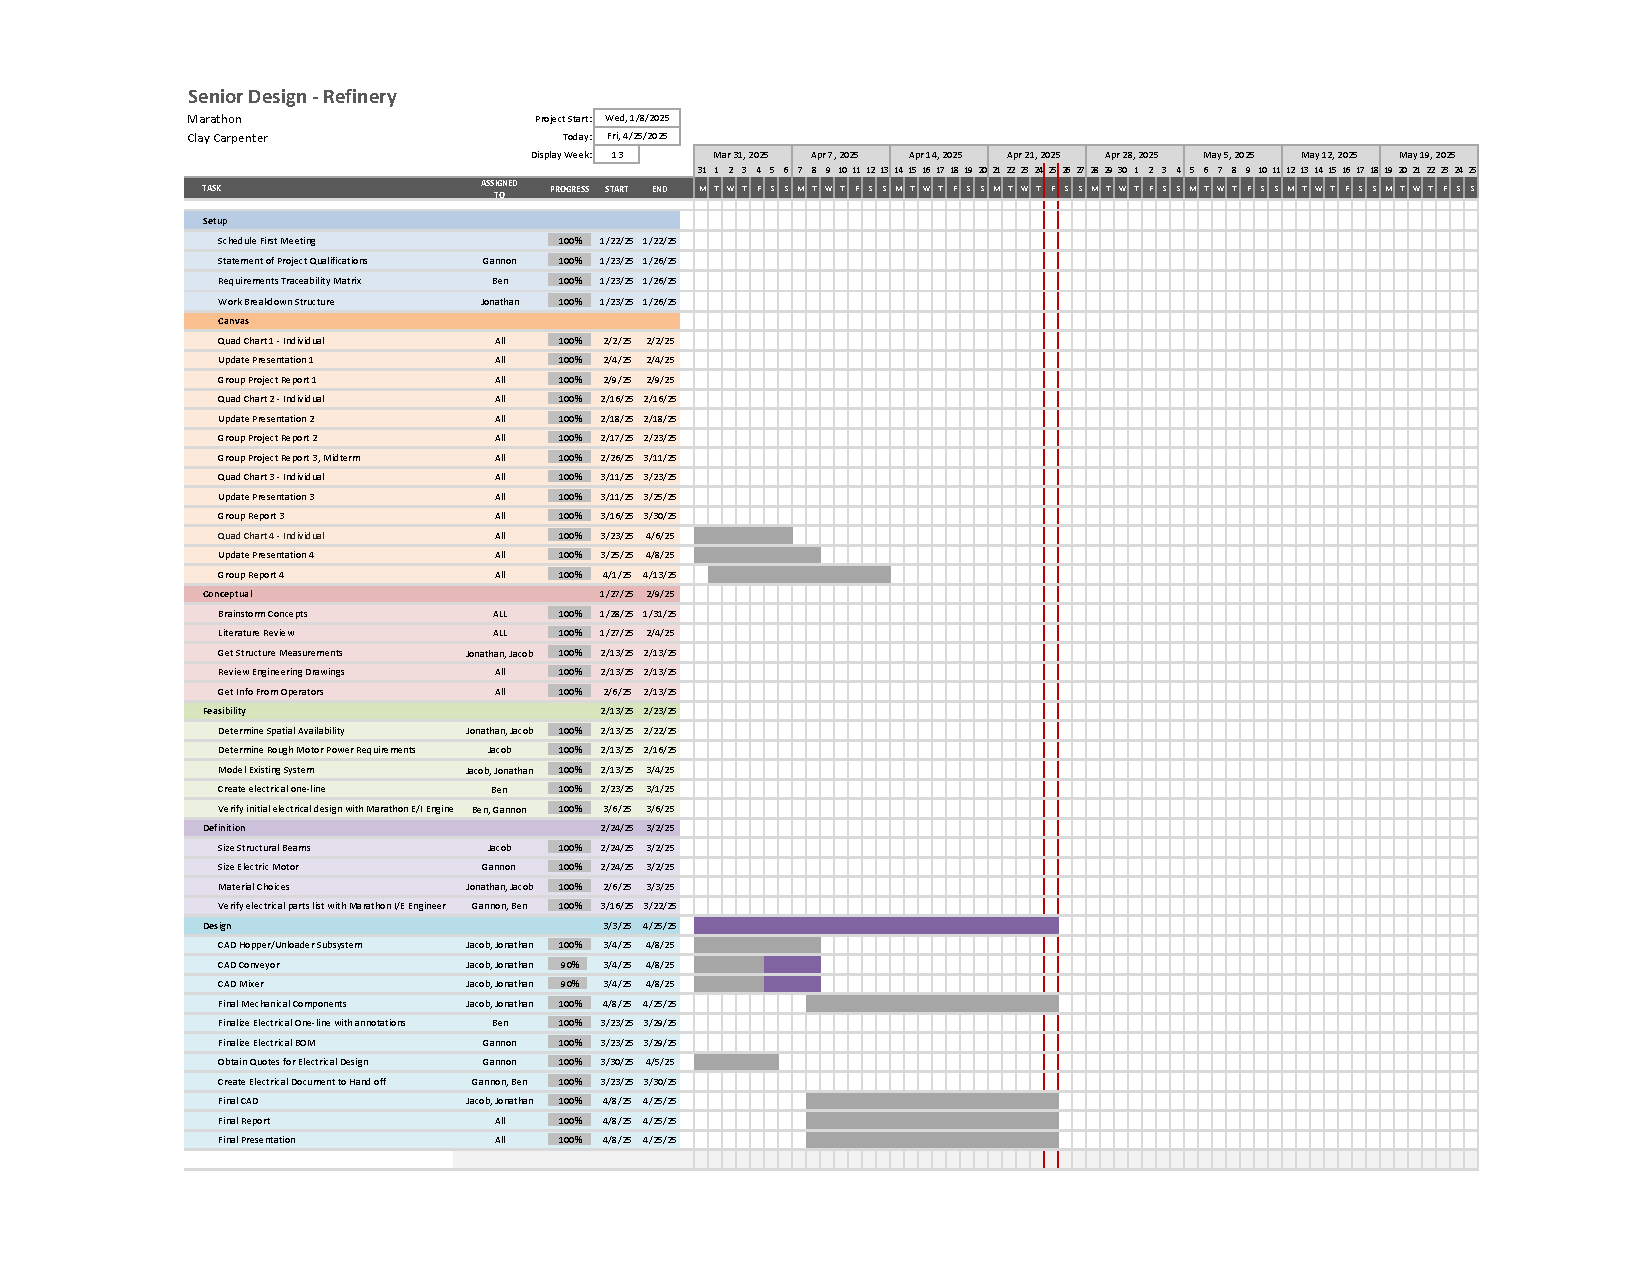
\includepdf[pages=1, fitpaper=true]{./Appendix/Senior Design Gantt Chart}

\subsection{Ideation, analysis, and selection}\label{sec:ide}%Needs to be updated

%You must show that in your early design phase, you engage in a systematic method whereby you generate ideas and then carefully consider and compare them based on their likelihood to satisfy your design requirements. One tool that you may choose to employ in this subsection is a decision matrix where you weigh your design ideas based on the likelihood that you assess they will satisfy your various design requirements.  You may also use lists of pros and cons or any of a variety of approaches to choosing between competing ideas.
%This subsection should be long enough to fully describe and illustrate your various design ideas. You should make use of preliminary CAD models in this subsection and other nice-looking methods of illustrating and explaining your various design ideas.

During the initial design and concept phase, the goal was to move the $CaCl_2$ pellets upward and into the hopper. Later it was made known that it was possible to transfer the pellets directly into the neutralization pit which was housed lower than the hopper meaning the pellets would only need to travel horizontally rather than vertically.
\subsubsection{Unloader}
Three main ideas came to mind when initially designing the unloading mechanism for the bulk bag unloader: Auger, Conveyor Lift, \& Gantry Crane.

The auger idea would function similarly to a classical auger seen on farms. $CaCl_2$ pellets would be loaded into a hopper at a lower level than currently used which would feed into an auger that would transfer them up to the chute level. This concept seemed simple as an auger would be bought but figured to be problematic due to the highly corrosive properties of $CaCl_2$, the limited customization of a purchased auger, and limited pad space.

The second concept is a conveyor lift. This functions similarly to the auger as the pellets are first unloaded at a lower level and then transferred higher. This would utilize a conveyor belt with buckets attached to it which would scoop $CaCl_2$ pellets little by little and then transfer them up to the chute. This design would be based off of a grain leg as seen in figure \ref{fig:grain leg} below:

\begin{figure}[H]
    \centering
    
\includegraphics[width=0.5\linewidth]{Senior Design Project Template//Figures/grain leg.PNG}
    \caption{Grain Leg, Bucket Elevator Conveyor Lift}
    \label{fig:grain leg}\cite{grainlegimage}
\end{figure}

The final design concept was a gantry crane. This would involve attaching the entire 2000-pound bag of $CaCl_2$ to a gantry crane where it would be hoisted from a lower ground level up into the place of the current bulk bag unloader. 
A comparison of each design concept can be seen below in table \ref{tab: weighted decision matrix}

%Insert weighted decision matrix

\begin{table}[H]
    \centering
    \begin{tabular}{|l|c|c|c|c|}
        \hline
        \textbf{Criteria} & \textbf{Weight} & \textbf{Auger} & \textbf{Conveyor Lift (Grain Leg)} & \textbf{Crane} \\
        \hline
        Safety Factor & 1.0 & 10 & 10 & 6 \\
        Estimated Cost & 0.5 & 8 & 7 & 8 \\
        Simplicity & 0.7 & 7 & 7 & 8 \\
        Reliability & 0.7 & 6 & 8 & 9 \\
        \hline
        \textbf{Total} & & 23.1 & 24 & 21.9 \\
        \hline
    \end{tabular}
    \caption{Comparison of Auger, Conveyor Lift (Grain Leg), and Crane}
    \label{tab: weighted decision matrix}
\end{table}


The table considers four main criteria: safety factor, cost, simplicity, and reliability. Safety has a weight of 1 giving it the highest importance. The crane scored much lower on the safety aspect than the other ideas since it would involve hoisting a one-ton bag above head level. The next criterion is estimated cost. Each design concept was similar in estimated cost here but the conveyor lift scored slightly lower since it was thought to have more custom parts rather than purchased. Simplicity was the next consideration with the crane scoring slightly better than the others. This was primarily because gantry cranes are commonplace in an industrial setting and have a large amount of easily accessible information about them making the design process simpler. The final factor was reliability. The auger got a low score here due to it being a large purchased part. If the auger needs maintenance, it may need to be serviced by external people rather than marathon technicians. The crane and conveyor lift have minimal components and were thought to be easier to maintain. 
Of the three ideas proposed, the conveyor lift came out on top with a score of 24. The design concept of a conveyor lift was chosen.\\\\% and the rest of the project design follows this idea.\\\\
After a closer inspection of the actual project site, it was determined that there was not a need to increase the elevation of the $CaCl_2$ pellets.  This was due to the pit being recessed into the ground and the walls of the pit being located at ground level.  Because of this, the design of the grain leg was slightly modified to make it move more horizontal instead of vertical.  Realizing that this concept shared many similarities with a conveyor belt system, it was decided to use a conveyor belt as the transportation device.
\subsubsection{Mixing}%Jonathan
\label{sec:Ideation-Mixer}
A secondary objective was to design a better mixing method.  The two general design paths considered were increasing the mechanical agitation in the pit, or dissolving the pellets in a liquid before the pit.\\\\  The liquefying method would consist of dissolving the pellets in a carrier liquid (most likely water), and then injecting the resulting solution into the pit.  This would completely solve the mixing problems.  However, such a system would be quite complex, requiring both an area to store and dissolve the pellets, a way to control the water content so as not to dilute the contents of the pit, and a way to collect and transport the resulting solution.  Additionally, because aqueous $CaCl_2$ solutions are rather corrosive, increased care would have to be taken to address the increased corrosion
\\\\
Mechanical agitation provided 2 possible designs.  The first would be a mixing device inserted directly into the pit that would stir the contents, increasing turbulence and helping the pellets dissolve faster.  This system would be unnecessarily difficult to maintain due to needing to be suspended over the center of the pit and being immersed in a corrosive environment.  The second design would be a modification of the existing air lance system, adding a pipe to the end of each lance that would direct the air towards the pellets, creating turbulence that would dissolve the pellets faster.
\subsection{Design Development} \label{sec:designDev}
%In this section you chronicle the development of your design both overall and for each subsystem. This section could be broken up into parts of your design and within each part you should illustrate the progression of your design (with cad models if appropriate) and discuss mathematical analyses you conducted and prototypes  you made and tested. Mathematical  analyses, simulation, demonstration, and testing are done for the sole purpose of evaluating a design against one of your design requirements. You have to be judicious and determine in what situations which verification methods are best.\\

The design development for this project can be divided into three distinct categories: the structural material used, the unloading structure, and the conveyor belt.
%The overall design of the Bulk Bag Unloader is split into two subsystems.  These subsystems are the unloader, which removes and stores the calcium chloride pellets from the bags; and the transport mechanism, moves the pellets into the pit.  Initially, a bucket elevator was planned to be used for the transport mechanism; however, the bucket elevator was replaced with a conveyor belt once it was discovered that the pit was recessed in the ground.
\subsubsection{Structural Material}\label{sec:Material}

Several considerations need to be taken into account when choosing which material to use for this project.  The first consideration is weldability.  As it is intended for the structural components to be welded together, the material chosen will need to be easily welded.  The second consideration involves the structure's location.  Due to being used around caustic chemicals, it is desired to construct the structure out of a material that is similar to those currently used by Marathon.  When liquid calcium chloride was used by Marathon, it was transported using ASTM 106 Grade B pipes.  As this rating is for pipes, it is ideal to find a similar analogue for non-pipe applications.  For this project, it was decided to go with A36 steel for the structural components.  This is a low carbon steel that is easily welded\cite{a36}.  Furthermore, the chemical composition and strength of A36 steel is close to the specified rating for A106 Grade B pipes.
Comparing Figures \ref{fig:a106_strength} and \ref{fig:a36_strength}, it can be seen that the rated minimum yield strength of A36 steel is within 4\% of the yield strength for A106 Grade B pipes, with A36 being rated with a slightly higher yield strength.  It can also be seen by comparing Figures \ref{fig:a106_chem} and \ref{fig:a36_chem} that the chemical composition of each is very similar.


\begin{figure}[H]
    \centering
    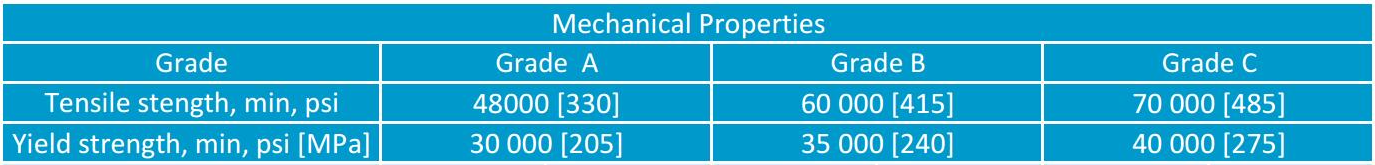
\includegraphics[width=1\linewidth]{./Images/a106_strength_2.png}
    \caption{A106 Strength\cite{a106}}
    \label{fig:a106_strength}
\end{figure}

\begin{figure}[H]
    \centering
    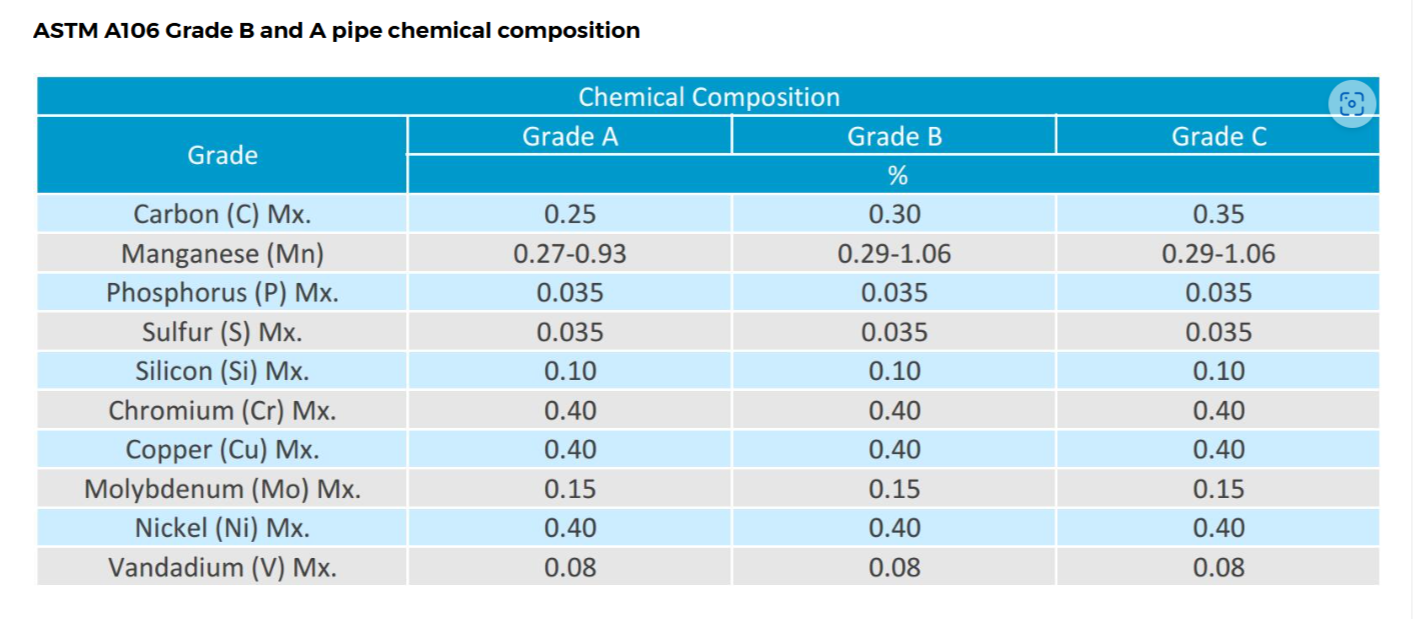
\includegraphics[width=1\linewidth]{./Images/a106_chem.PNG}
    \caption{A106 Chemical Properties\cite{a106}}
    \label{fig:a106_chem}
\end{figure}

\begin{figure}[H]
    \centering
    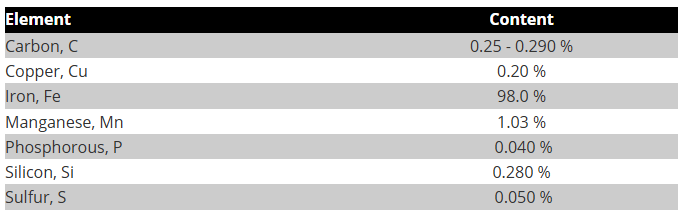
\includegraphics[width=1\linewidth]{./Images/Materials/a36_chem.png}
    \caption{A36 Chemical Properties\cite{a36}}
    \label{fig:a36_chem}
\end{figure}

\begin{figure}[H]
    \centering
    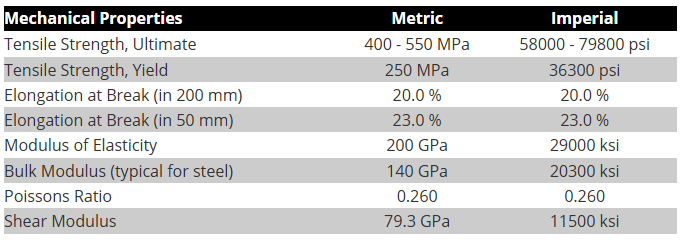
\includegraphics[width=1\linewidth]{./Images/Materials/a36_strength.png}
    \caption{A36 Strength\cite{a36}}
    \label{fig:a36_strength}
\end{figure}


\subsubsection{Unloader} \label{sec:designUnload}
One of the main goals when designing the unloader was to move it closer to the ground.  Currently, the unloader sits around 18 feet in the air. The operators utilizing the bulk bag unloader had an ideal maximum lift height of 12 feet.  At this height, the bag should be able to be mounted safely by an operator using a forklift or a telehandler.
The bulk bags being utilized to transport the $CaCl_2$ are seven feet tall.  In addition, if the operators are to cut the bag by hand, they will require around two feet of access under the bag.  Adding these numbers together, one will see that these requirements only leave around three feet of height to design the storage part of the unloader.  One way to solve this is to utilize a cutting mechanism.  The current bulk bag unloader has a mechanism on it that will cut the outlet pipe of the bag.  This allows the bottom of the bag to feed straight into the hopper, thus eliminating the need for additional access space.  It also allows the system to be completely enclosed, providing protection from the elements to the $CaCl_2$.\\\\
\noindent Once the bag has been cut, a system is needed to control the mass flow rate of the $CaCl_2$ entering the conveyor system to a rate slower than that of the material leaving the bag.  Two different methods were looked at to accomplish this.  The first was to do so passively. 
 Using a passive system would limit the complexity of the system; however, it would also take away control from the operator to determine exactly how much $CaCl_2$ to deliver to the pit at a time.  This method would be accomplished by designing the size of the exit from the hopper to the conveyor belt to only allow the desired amount of pellets through.  The other method would be to utilize a slide valve like the one already in use.  This would allow the amount of material delivered to be more controllable, but it would make the system more complex.\\\\
\noindent Due to the hygroscopic nature of $CaCl_2$, it is expected that at some point during operation, the hopper will get clogged due to clumping of the pellets.  To account for this, an access hatch will need to be installed on the hopper.  This will allow the operator to gain access to the inside and safely and quickly clear any clog that forms.\\\\
\noindent Taking all of these into consideration, it was decided to reuse the current cutting and delivery system already located on site.  The current system already has a cutter, hopper, and slide valve system configured to accept the bulk bags.  In addition, the current hopper has an access point to allow for clearing of any possible clogs.  By reusing the existing setup, Marathon will be able to minimize the cost of this project.  All the parts that are being reused can be seen in Figure \ref{fig:assem}.

\begin{figure}[H]
    \centering
    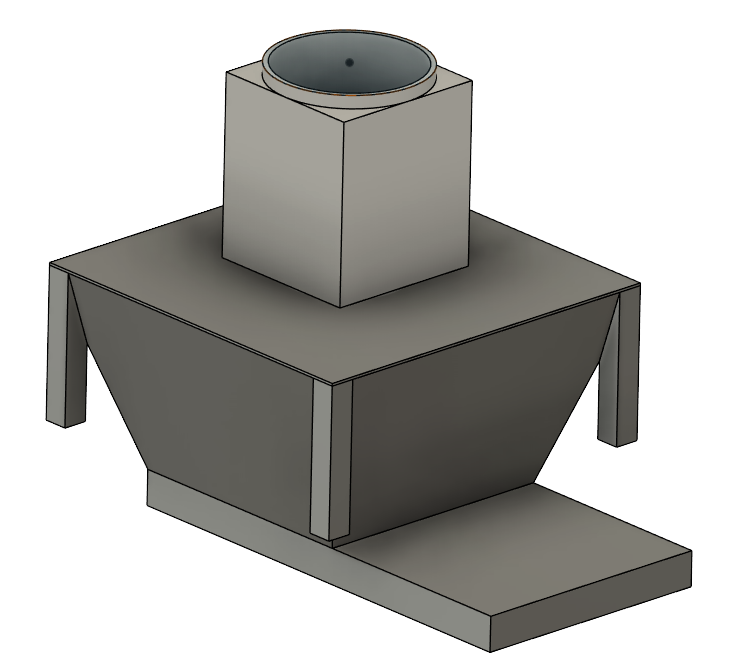
\includegraphics[width=0.5\linewidth]{./Images/Structure/valveassembly.png}
    \caption{Components Being Reused}
    \label{fig:assem}
\end{figure}

\noindent The current structure has a spring-loaded adjustment mechanism on each of the four corners.  This is intended to provide adjustibility in the system.  Because of this, it was decided to construct a whole new structural system instead of modifying the current system, as it was simpler to construct a new system than to modify the existing structure around the spring mechanisms.  It was decided to use the existing mounting points on the pad for simplicity.  The new system can be seen in Figure \ref{fig:new}.  For the four support pillars, it was decided to use 4"x4"x.25" A500 Grade B steel tubing.

\begin{figure}[H]
    \centering
    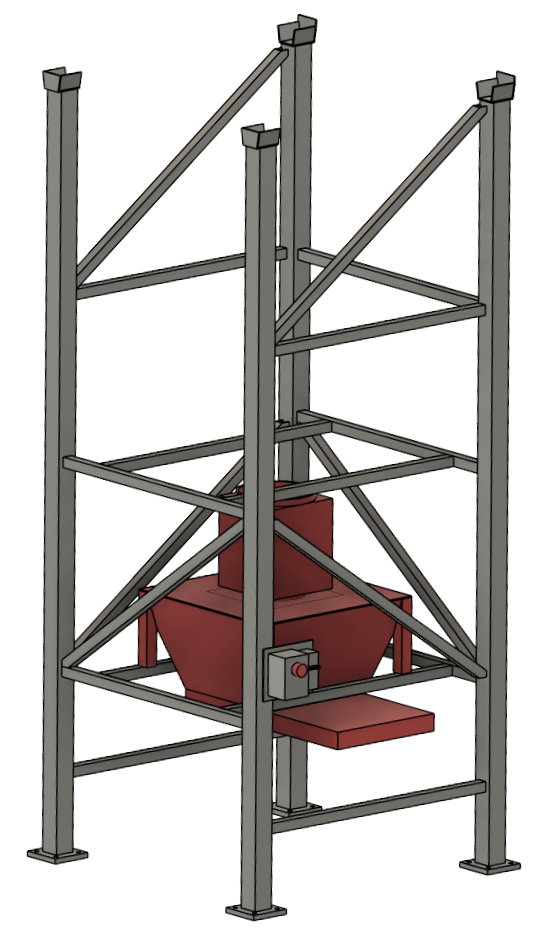
\includegraphics[width=0.6\linewidth]{./Images/Structure/nobag2.png}
    \caption{New Bulk Bag Unloading Structure using Existing Cutter, Hopper, and Slide Valve (Red)}
    \label{fig:new}
\end{figure}

\noindent Because of the height and weight that the support pillars are experiencing, it was important to guarantee that they would not fail.  Three failure criteria were analyzed: bending failure, axial failure, and buckling.  The first failure method that was examined was bending failure.  Due to the large weight that could be experienced and the tall height of the system, it was assumed that this would be the most critical failure mode to consider.  The first tubing choice examined was a 3"x3" tube with 1/4" thick sidewalls.  It was discovered that this tube would not be able to support the load applied in a scenario where the structure experienced 500 lbs applied horizontally to the top of each corner .  The next tubing size analyzed was a 4"x4" tube with 1/4" thick sidewalls.  This beam was found to be able to withstand the worst case bending scenario with a safety factor of 2.71.  Next, this beam choice was analyzed for axial failure.  As expected, this was shown to have a high safety factor of 345.  Finally, the beam was analyzed for buckling.  It was shown that each individual beam could support 28,075 lbs before buckling.  This means there is a safety factor of 56.15 against buckling.  These calculations justified the decision to move forward with using 4"x4" A500 Grade B tubing for the support pillars.


\subsubsection{Conveyor Belt} \label{sec:designBelt}
To accomodate the requested flow rate of $CaCl_2$, it was decided to make the belt as wide as the unloader will support, as this will increase the amount of material that can be moved at a time for a given rpm.  This choice also had benefits when considering the troughed design.  With troughed belts, the important factor to consider is the trough angle.  As this is increased, the ability of the belt to center any material it is carrying increases, while at the same time increasing the required flexibility of the belt material.  Because this belt needs to operate at subzero temperatures and the availability of material that has high flexibility at subzero temperatures is minimal, it was decided to keep the trough angle small.  This decision will have little impact on material spillage as the outlet of the slide valve is small compared to the maximum width of belt supported by the unloader.
\\\\
Because of the similarity in loading conditions to the unloader, it was decided to use the same steel extrusion used on that structure.  This serves to reduce the number of unique materials that will need to be sourced and will make the conveyor frame easier to manufacture.



\section{Results and Discussions}\label{sec:discuss}

%Presents the data generated in the project relative to the design specifications and objectives defined for the project in order to enable an assessment of the success of the project. An assessment of the project’s success, with justification, shall be made. Known limitations and issues with the design project should be discussed in this section. Significant challenges encountered and deviations from the original plan should be included.

With the requirements laid out at the beginning of this project, the final design of the unloading structure has been shown to meet those requirements.  Through calculations and conducting a Finite Element Analysis, the structure and material choices have been shown to be able to withstand the weight of the bulk bag.  While the overall height is slightly over the 12 foot limit that was set, it is not that much over, and certain future improvements could be undertaken to make the structure even shorter.\\
It is less clear if the conveyor belt is successful.  Due to the need to redesign the transportation method from the original plan, it is not as well defined as the unloading structure.  One major limitation with the conveyor belt is the material used for the belt.  It is not rated for as cold as was desired for use in North Dakota, but it was the only option that this group was able to get information about from the company that provides it.  This is a point that definitely needs future development on to be implemented successfully.\\
The mixing mechanism can also be deemed successful.  By modifying the existing system to direct the airflow more directly towards the $CaCl_2$, the pellets will be able to experience more turbulent movement, which will stimulate more even dissolution into the contents of the neutralization pit.  With the addition of a flange, the replacement and repair of this system will be more efficient for the operators.  One limitation of the system is the wear of the system due to the induced moment from the air leaving the pipe.  Since the pipe is braced against the wall, it will be important to monitor the effect the movement of the pipe has on the wall.  If the wall is observed to be worn down by the movement of the pipe, a pipe sock will have to be added to counteract this behavior.\\
The electrical system can also be deemed a success with regards to the initial requirements.  Each component is rated for Class 1 Division 2, and are thus safe to be installed in the refinery.\\
As mentioned above, a major redesign was necessary within the development of this project.  Due to having limited access to the site location early on, certain assumptions were taken that there would be a necessary requirement to transport material vertically to at least the height of the existing chute.  Because of this assumption, steps were initially taken to design a structure that could meet that requirement.  After finally getting on site and realizing that vertical movement would not be necessary, the design was re-evaluated and a new design concept was determined to be better.  Because of this change in design, much of the design work that had been previously accomplished was not useful for the new system design.

\section{Future Work}\label{sec:future}
Despite all the work that was put into this project this semester, there are still a few areas that could use improvement.  Four main areas that would want to be improved on before implementation are a protective cover for the conveyor belt, designing the unloading structure to split in two, changing the conveyor belt material, and protecting the structural steel from the elements.
%Based upon the results obtained, recommended future work related to the process or product should be discussed. 
\subsection{Conveyor Belt Cover}
Because the conveyor belt is sitting outside, it is important to protect it from the environment.  While the steel is protected by a coating, parts like the motor, pulleys, and bearings cannot be protected this way.  An idea to create a removable structure that would sit over the conveyor belt was posited.  This structure would be made of steel tubing and sheet metal, and would consist of multiple removable sections.  This would allow it to protect all the more sensitive components of the conveyor belt, as well as be easily removable for any cleaning or maintenance that would need to take place.
\subsection{Splitting the Unloading Structure}
When meeting with Marathon, the idea was brought up to modify the design so that the top half could be removed.  This would allow the $CaCl_2$ bag to be loaded at a lower height, then lifted up and placed on the rest of the structure.  While the overall height would be the same, the forklift would not need to extend as high as it would be lifting from the bottom of the bag rather than the top.  This idea showed a lot of promise; however, it was presented to late in the semester to be analyzed fully and implemented.  It would be a good place to begin for any future improvements that are to be made to the system.
\subsection{Conveyor Belt Material Choice}
Due to North Dakota's extreme winters, a belt that can remain operable below -40$\degree C$ is desired.  During the research portion of this project, it was discovered that the company Fenner Dunlop manufactures conveyor belts that are rated for -60 $\degree C$; however, they would not respond when reached out to.  Further follow ups with them or a company with a similar conveyor belt offering would be another step that could be taken to further develop this project.
\subsection{Protecting Structural Steel}
Due to the exposure to the elements, it is important to apply some sort of protective coating to the structural steel to prevent it from rusting.  The initial plan at the start of this project was to use the same coating that is used on the existing structure, which is an enamel coating with stainless steel additives called "Steel-It."\cite{steel-it}  However, it is uncertain if this is the best or most cost effective option to accomplish the job.  Further investigation into other forms of rust protection, such as paint, would be important before implementing this structure.
%The electrical design has been fully completed. 
\subsection{Mixing System Refinement}
\label{sec:MixingSystemRefinement}
Because the amount of pellets dumped into the pit and the amount and strength of the spent liquid to be neutralized varies so much, it was difficult to accurately model and design a proper length for the horizontal pipe or an optimal angle at which to angle them.  Therefore, further testing would need to be done on-site to determine how the pellets behave when subjected to this new turbulence and what lengths and angles of pipe outlets would provide the best dissolving rate.  Such iterative testing shouldn't be too difficult considering the simplicity and low-cost of the system as well as its status as a consumable object. 



\section{Summary and Conclusion}

This project addressed the need for an improved system for unloading 2000-lb bulk bags of calcium chloride (CaCl2) and mixing it into the neutralization pit at the Mandan Marathon Oil Refinery. The primary objectives were to enhance operator safety and ergonomics during the unloading process, increase the efficiency of CaCl2 transport, improve dissolution and reduce clumping in the neutralization pit, and ensure the entire system complies with safety regulations, particularly Class 1 Division II electrical standards for hazardous locations.
\\\\
The resulting design proposes a comprehensive solution featuring a redesigned lower unloading structure constructed from A500 Grade B steel, facilitating safer bag handling at a maximum height of 12 feet while reusing key existing components such as the cutter, hopper, and slide valve to manage costs. A horizontal trough conveyor belt system, driven by a C1D2-rated 1 HP motor with a 100:1 gearbox, was designed to reliably transport CaCl2 pellets from the unloader to the pit at a calculated rate exceeding 10,000 lbs/hour. Furthermore, an enhanced mixing system utilizing modified air lances directs airflow to create turbulence at the pellet entry point, promoting better dissolution. The electrical system design meticulously follows the NEC guidelines, incorporating appropriate C1D2 enclosures, conduit, and safety controls such as an emergency stop.
\\\\
This design provides a significant improvement over the existing system by directly addressing the identified safety hazards and operational inefficiencies. Lowering the unloader improves ergonomics, the conveyor provides controlled material transport, and the modified air lances target mixing problems. The adherence to stringent safety codes and careful material selection ensure the suitability and reliability of the system within the demanding refinery environment, ultimately contributing to a safer and more efficient chemical handling process at the Mandan Refinery.

\section{References}

\let\seccs=\section
\renewcommand{\section}[2]{}%

\begin{thebibliography}{20}
%
\bibitem{hibbler} Hibbler RC, {\it Mechanics of Materials}, Upper Saddle River, N.J: Pearson Education, 2003. Print.
%

\bibitem{grainlegimage} {\it The prairie skyscraper} Amy Bickel, illustration by Jim Heck Kansas Agland, The Hutchinson News, July 3, 2016.
\url{https://www.hutchnews.com/story/news/local/2016/07/03/the-prairie-skyscraper/20979484007/}

\bibitem{Oravcová} {\it Corrosion of metals in zinc nitrate hexahydrate and calcium chloride hexahydrate.}, Acta Chimica Slovaca, vol. 11, no. 1, Apr. 2018, pp. 51–54. EBSCOhost. 
\url{https://doi-org.ezproxy.umary.edu/10.2478/acs-2018-0008}

\bibitem{Class and Division} {\it Class and Division: Don't Break Rank on Your Next Installation.},  EC\&M Electrical Construction \& Maintenance, February 2006, pp. 48-53. 
\url{https://research-ebsco-com.ezproxy.umary.edu/c/fg2nyx/viewer/html/kyojggainb}



\bibitem{BritishStainless} {\it Selection of Stainless Steels for Handling Hydrofluoric Acid (HF)}, British Stainless Steel Association. 
\url{https://bssa.org.uk/bssa_articles/selection-of-stainless-steels-for-handling-hydrofluoric-acid-hf/}

\bibitem{conveyor} {\it The Complete Guide to Industrial Conveyor Selection, Configuration, and Troubleshooting.}, Feeco International. 
\url{https://feeco.com/the-complete-guide-to-industrial-conveyor-selection-configuration-and-troubleshooting/}

\bibitem{SuperMetals} {\it Which alloy is best for use in hydrofluoric acid applications?}, Heanjia Super Metals. 
\url{https://super-metals.com/news/which-alloy-is-best-for-use-in-hydrofluoric-acid-applications/}
%%%%%%%%%%%%%%%%%%%%%%%%%%%%%%%%%%%%%%%%%%%%%%%%%%%%%%%%%%%%%%%%%%%%
% Jacob's Citations: Work in Progress, Will finish when free
%%%%%%%%%%%%%%%%%%%%%%%%%%%%%%%%%%%%%%%%%%%%%%%%%%%%%%%%%%%%%%%%%%%%

%\bibitem{main_beam} {\it Design and Analysis with Numerical Method of Gantry Crane Main Beam},%  EC\&M Electrical Construction \& Maintenance, February 2006, pp. 48-53. 
%\url{https://research-ebsco-com.ezproxy.umary.edu/c/fg2nyx/viewer/html/kyojggainb}

%\bibitem{redline}
%\url{https://www.redlinesystems.com/conveyor-calculations-for-proper-design/#:~:text=Belt%20Load%201%20When%20the%20load%20is%20per,%2F%20%28S%20x%2060%29%20x%20C%20%28in%20feet%29}

\bibitem{a106}\textit{ASTM A106 Grade B Pipe Specification}, Octal Steel.
\url{https://www.octalsteel.com/astm-a106-grade-b-pipe/}


\bibitem{Marathon}Marathon - Mandan Refinery.

\bibitem{auger}Jones, Dr. Carol E., \textit{Auger Conveyors}, Oklahoma Cooperative Extension Service.
\url{https://extension.okstate.edu/fact-sheets/print-publications/bae/auger-conveyors-bae-1105.pdf}

\bibitem{grain_leg}\textit{Grain Elevators}, University of Regina and Canadian Plains Research Center.
\url{https://esask.uregina.ca/tmc_cms/modules/customcode/includes/print_entry.cfm-entryid=7349CBF7-1560-95DA-43A44D3266A89508.html}

\bibitem{globalspec}\textit{Augers Information}, GlobalSpec.\url{https://www.globalspec.com/learnmore/building_construction/building_construction_tools_machines/augers}

\bibitem{jane} Ross, Jane.  \textit{Grain Elevators}, The Canadian Encyclopedia, April 24, 2015.
\url{https://www.thecanadianencyclopedia.ca/en/article/grain-elevators}

\bibitem{maxim}\textit{Unlocking The Power of Gantry Cranes: A Guide to Efficient Lifting}, Maxim Crane Works, 6 July 2023.\\
\url{https://www.maximcrane.com/blog/unlocking-the-power-of-gantry-cranes/}

\bibitem{wallace}\textit{Electric Gantry Hoists}, Wallace Cranes.
~\url{https://www.wallacecranes.com/wp-content/uploads/2014/03/ER2ModB_2Ton_wbag.jpg}

\bibitem{donqi}Donqi Crane.
~\url{https://www.eotcranekit.com/uploads/20220815/1dd4552863e14eff5a51291533775343.jpg}

\bibitem{harbor}\textit{Haul-Master 1 Ton Push Beam Trolley}, Harbor Freight.
\url{https://www.harborfreight.com/1-ton-push-trolley-97392.html}

\bibitem{marcel}Eijpe, Dr. Michiel, \textit{It's Cold Outside!  A Guide to Rubber Conveyor Belts Operating in Extreme Cold Conditions}, Fenner Dunlop Conveyor Belting, 12 March 2020.
\url{https://www.fennerdunlopemea.com/app/uploads/2020/03/2020_Mar_Bulk-Blog_Its-cold-outside.pdf}

\bibitem{iqs}\textit{Belt Conveyors: Types, Components, and Applications}, Industrial Quick Search.
\url{https://www.iqsdirectory.com/articles/conveyors/belt-conveyors.html}

\bibitem{a36}\textit{ASTM A36 Mild/Low Carbon Steel}, AZO Materials.
\url{https://www.azom.com/article.aspx?ArticleID=6117}

\bibitem{SSINA}\textit{Chloride Stress Corrosion Cracking}, SSINA.
\url{https://www.ssina.com/education/corrosion/chloride-stress-corrosion-cracking/}

\bibitem{a500}\textit{ASTM A500 Steel Properties}, Beam Dimensions.
\url{https://beamdimensions.com/materials/Steel/ASTM/ASTM_A500/}

\bibitem{buckling}\textit{Euler Column Buckling: Formula, Theory, Calculator}, The Engineering Toolbox.
\url{https://www.engineeringtoolbox.com/euler-column-formula-d_1813.html}

\bibitem{steel-it}\textit{STEEL-IT Steel Gray Polyurethane 1 Gallon STL1002G}, Signature Motorsports.
\url{https://signaturemotorsports.com/steel-it-steel-gray-polyurethane-1-gallon-stl1002g/?gad_source=1&gbraid=0AAAAApVQqNuNDTteAdz7Xq1FnVvjFBZv0&gclid=Cj0KCQjw5azABhD1ARIsAA0WFUGB6Y-hbN5q96dGfFCJedahTJWARGg3W22NOY0PcZgiM3jybzaUIfgaAgYTEALw_wcB}

\end{thebibliography}

%\bibliographystyle{unsrt}
%\bibliography{references}{}

% Here I am restoring the original definition of the section command to generate section titles again
\let\section=\seccs

\section{Appendix}\label{Appendix}
%If applicable, large data sets, collections of photos, and step-by-step procedures for manufacturing materials or conducting tests will be included here. Drawing packets, BOMs, construction documents, detailed circuit/system diagrams, and code will be stored here.  Applicable standards may also be attached if they are not excessively long.  Material shall be organized into multiple appendices as necessary, using an uppercase alphabetic identifier (e.g., Appendix A). If an appendix is not required, the section shall be deleted. \\





\subsection{Conveyor Belt}\label{pdf:belt}

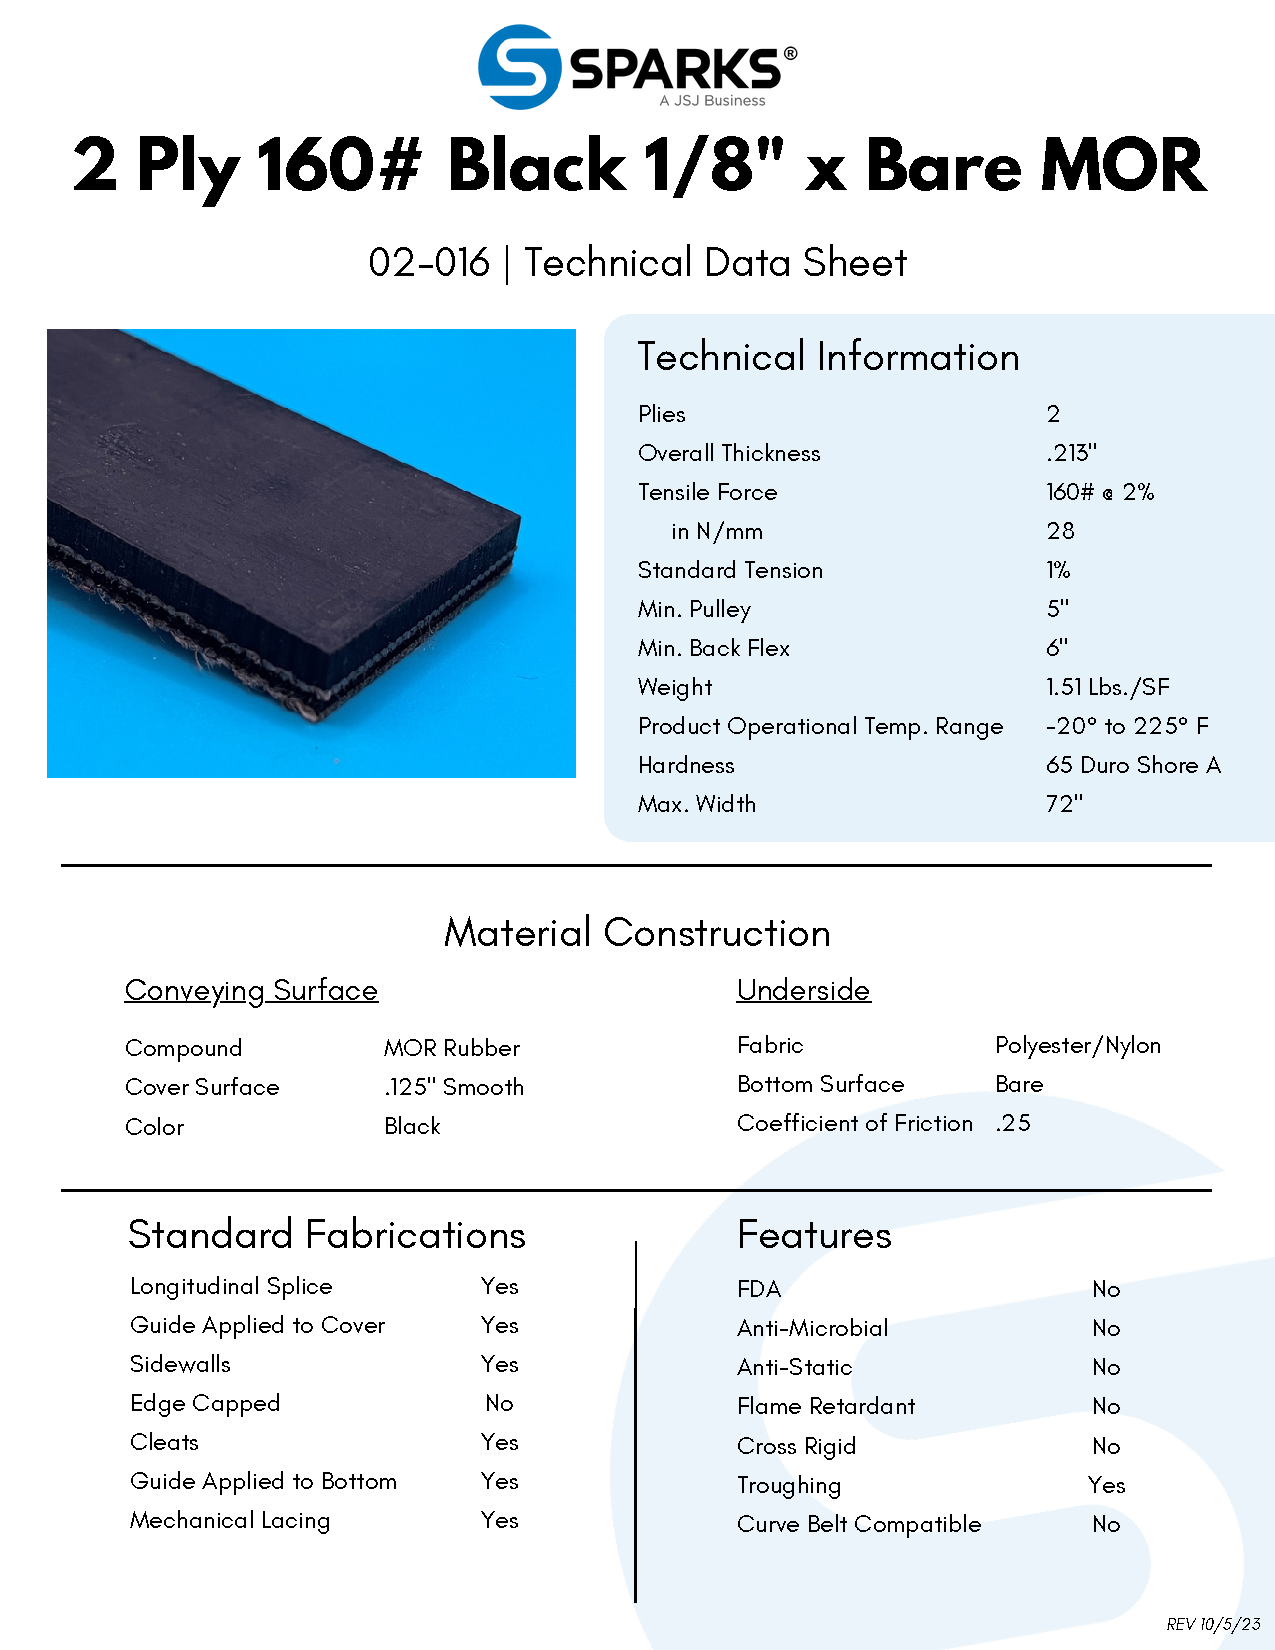
\includepdf[pages=-]{./Appendix/02-016-2-Ply-160-Black-18-x-Bare-MOR.pdf}

\subsection{Bulk Bag}\label{sec:bulk}

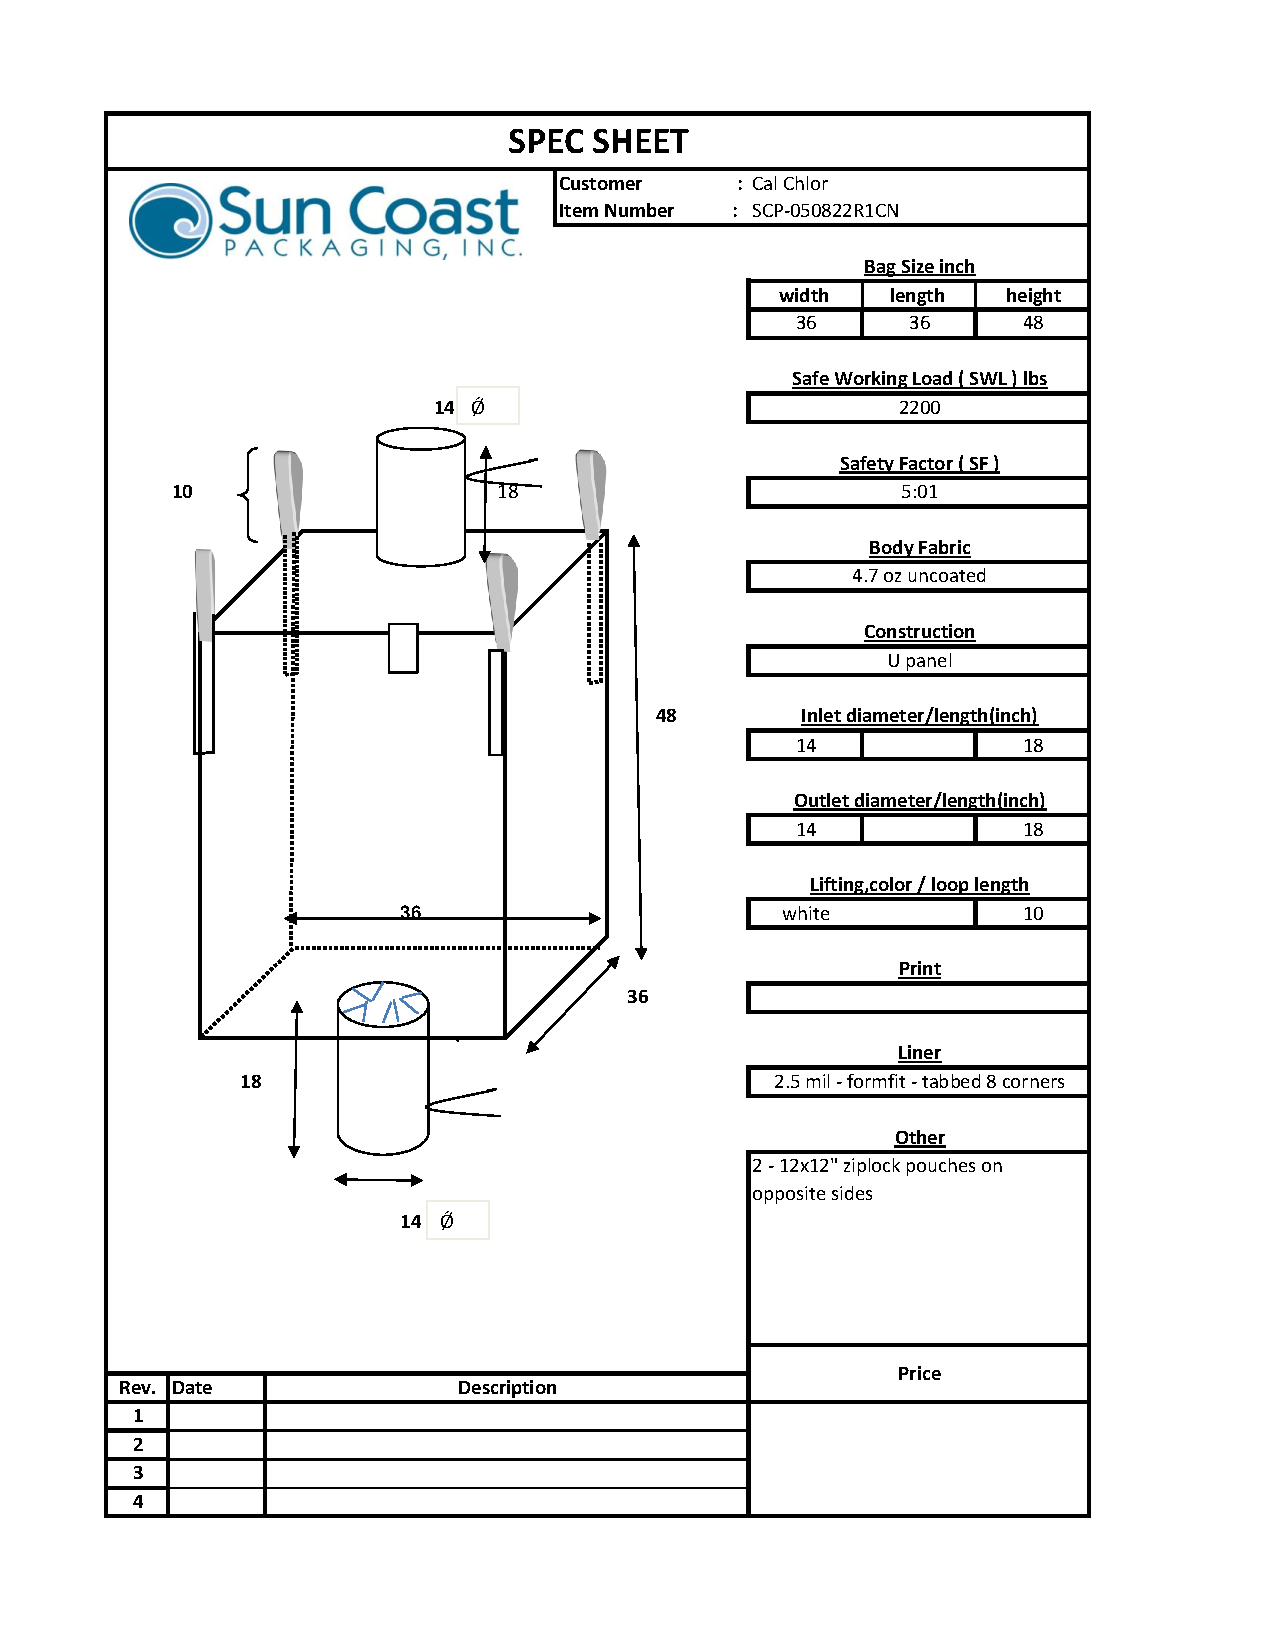
\includepdf[pages=-]{./Appendix/Bulk Bag/Dimensions - Domestic 2000 Pound Bag.pdf}
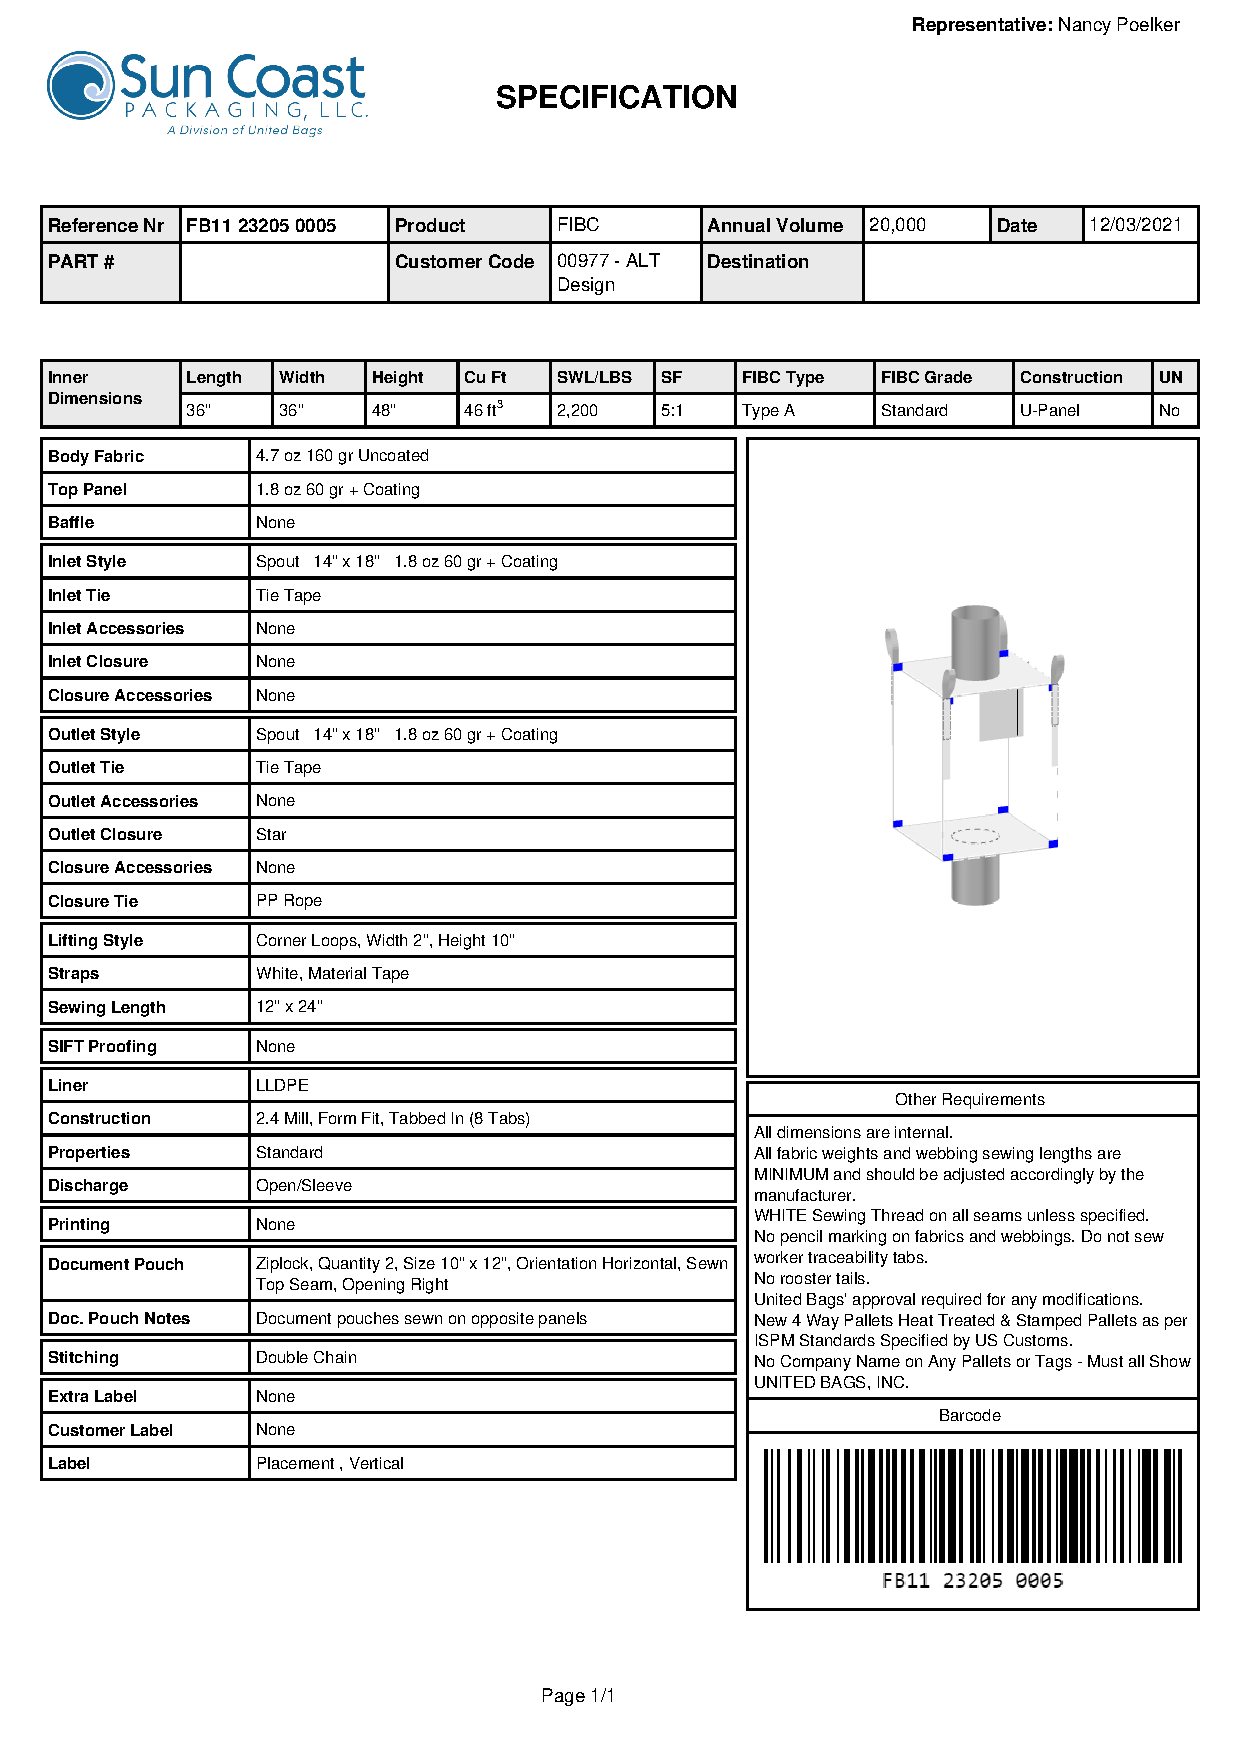
\includepdf[pages=-]{./Appendix/Bulk Bag/Dimensions 2 - Domestic 2000 Pound Bag.pdf}

\subsection{Gearbox}
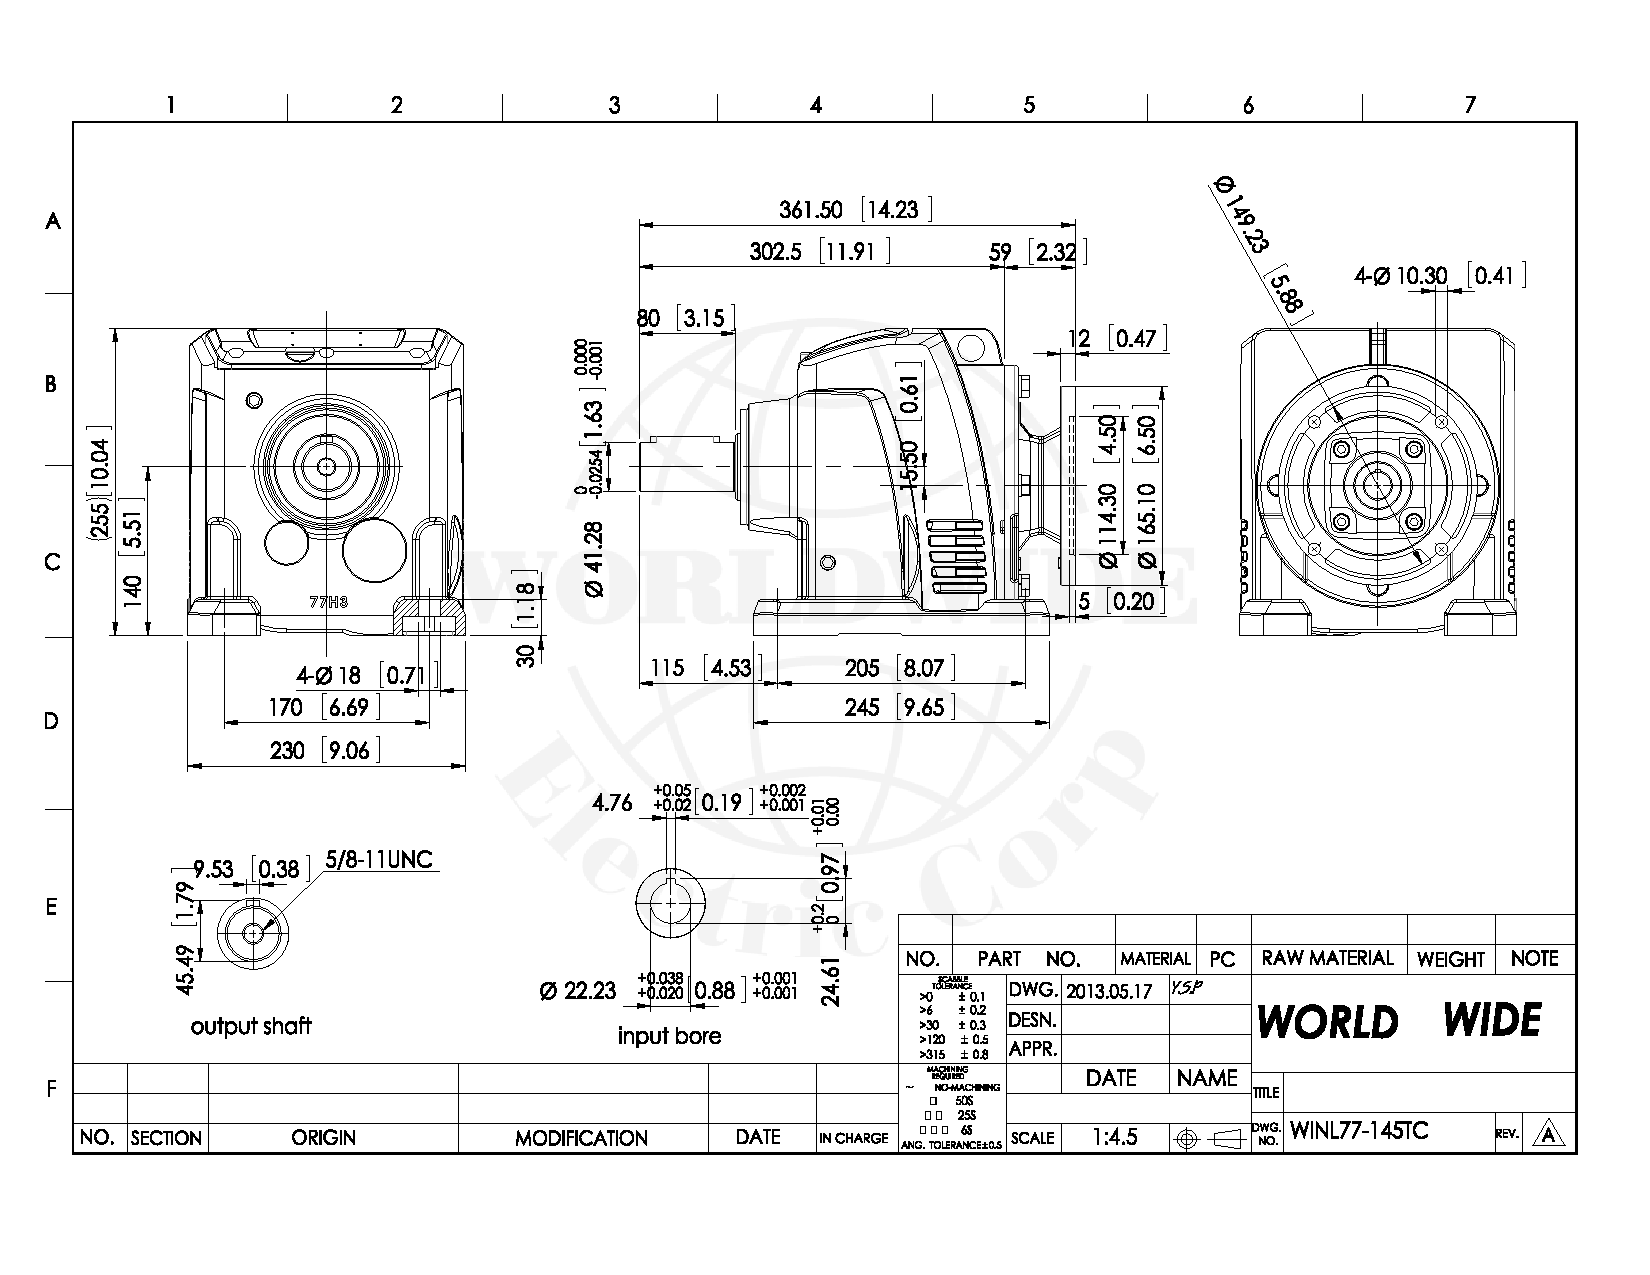
\includepdf[pages=-, fitpaper=true]{./Appendix/WINL77-145TC Gearbox.pdf}
\subsection{Demolition Plan}\label{sec:demolish}

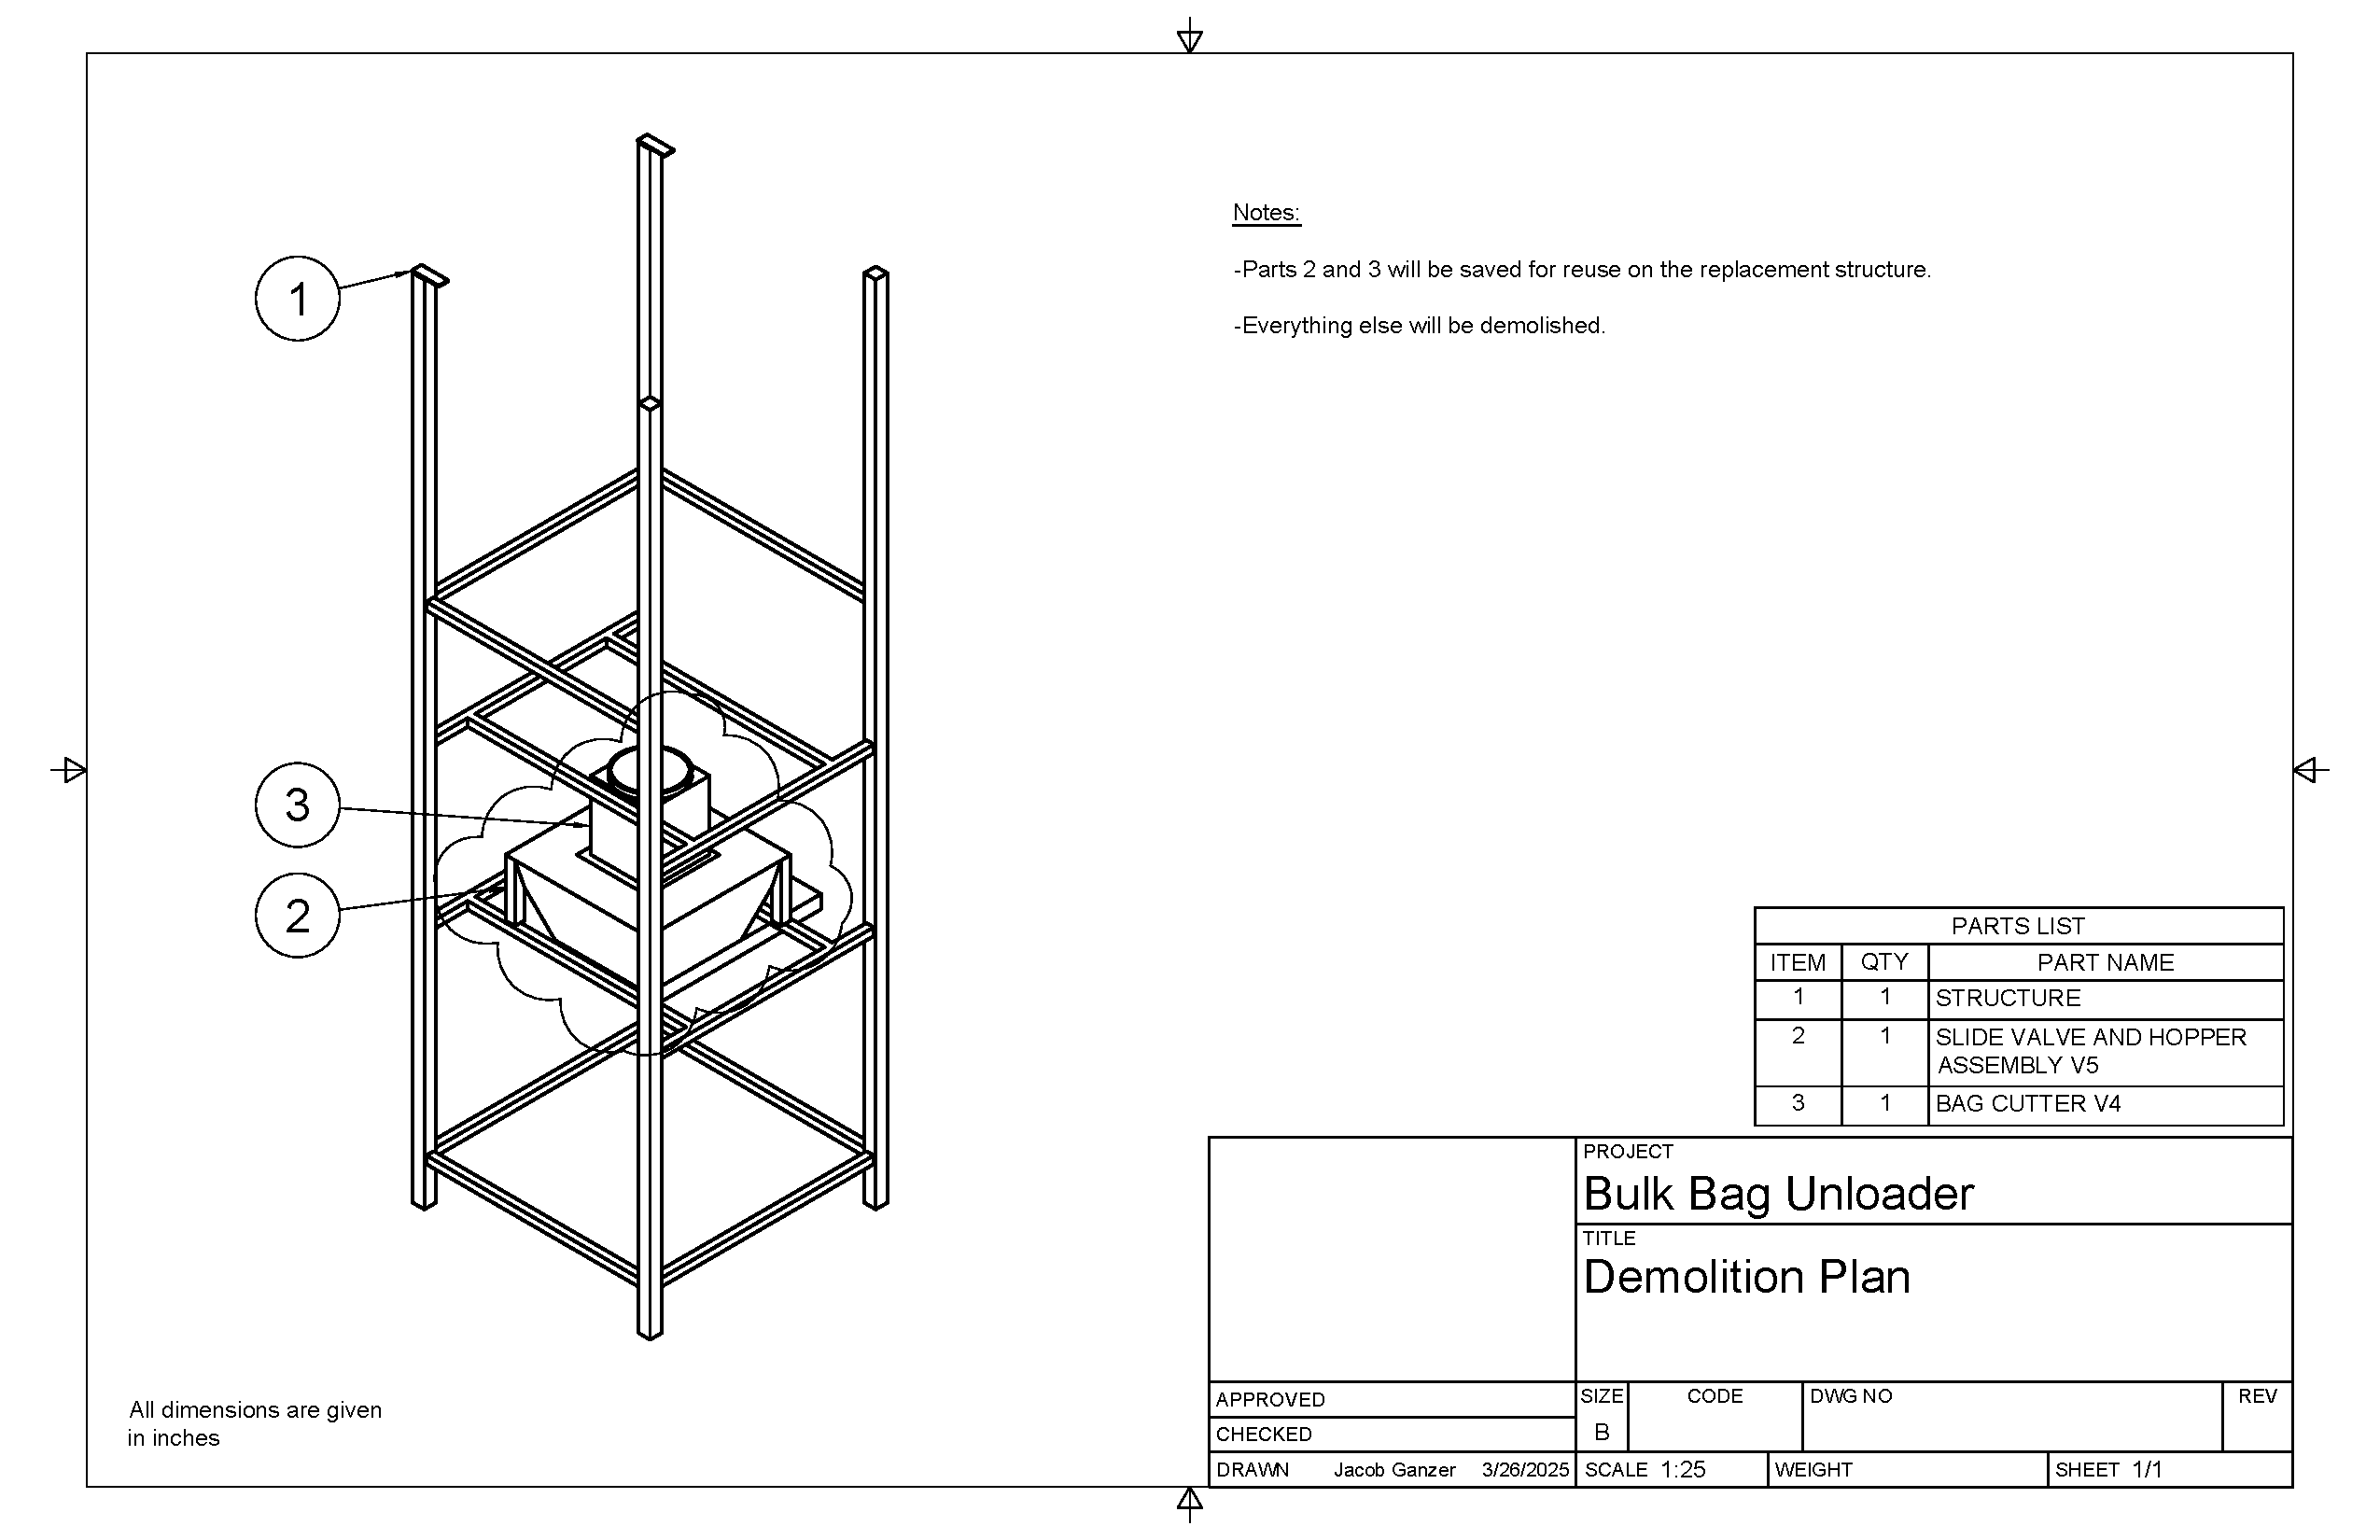
\includepdf[pages=-, fitpaper=true]{./Appendix/Unloader/DemolitionPlan v11.pdf}

\subsection{Structure}\label{sec:drawing}
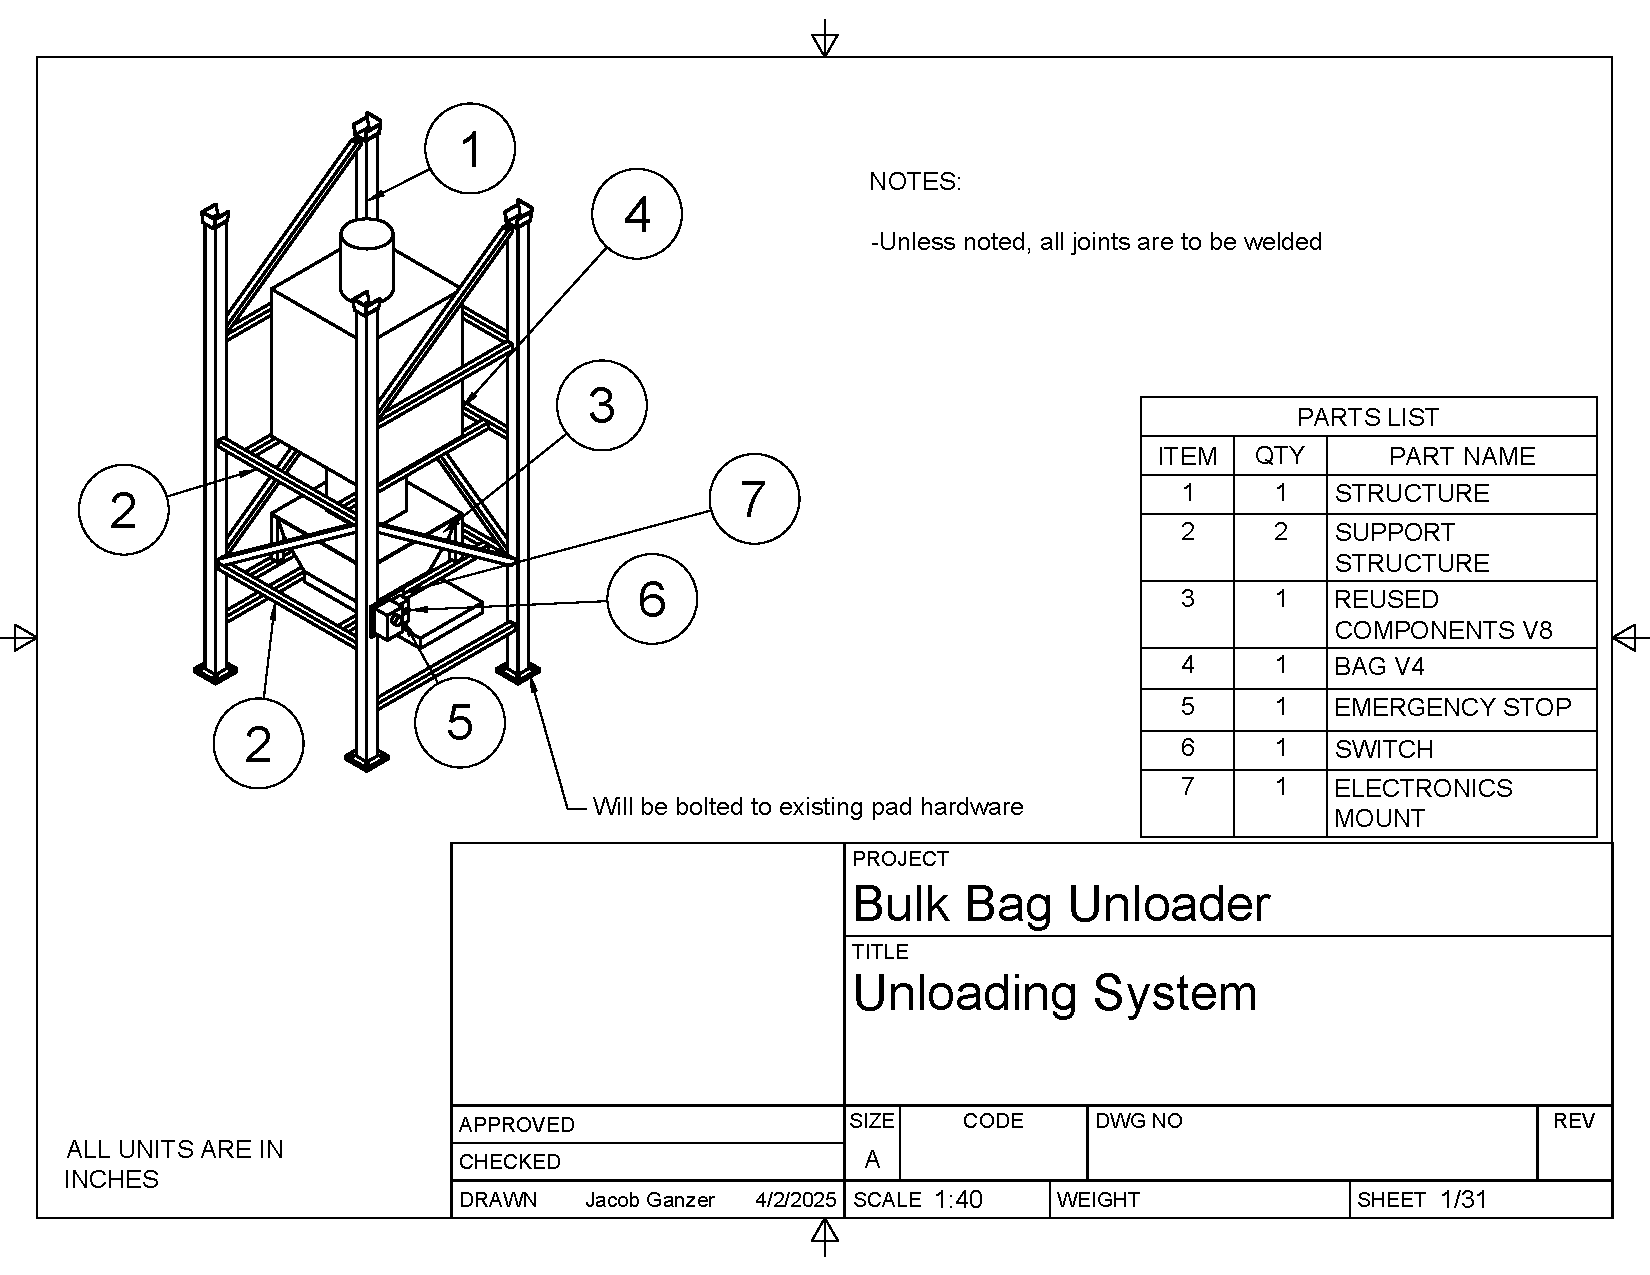
\includepdf[pages=-, fitpaper=true]{./Appendix/Unloader/NewStructure2 Drawing v34.pdf}

\subsection{Conveyor System}\label{pdf:conveyor}
%\includepdf[pages=-, fitpaper=true]{PLACEHOLDER}
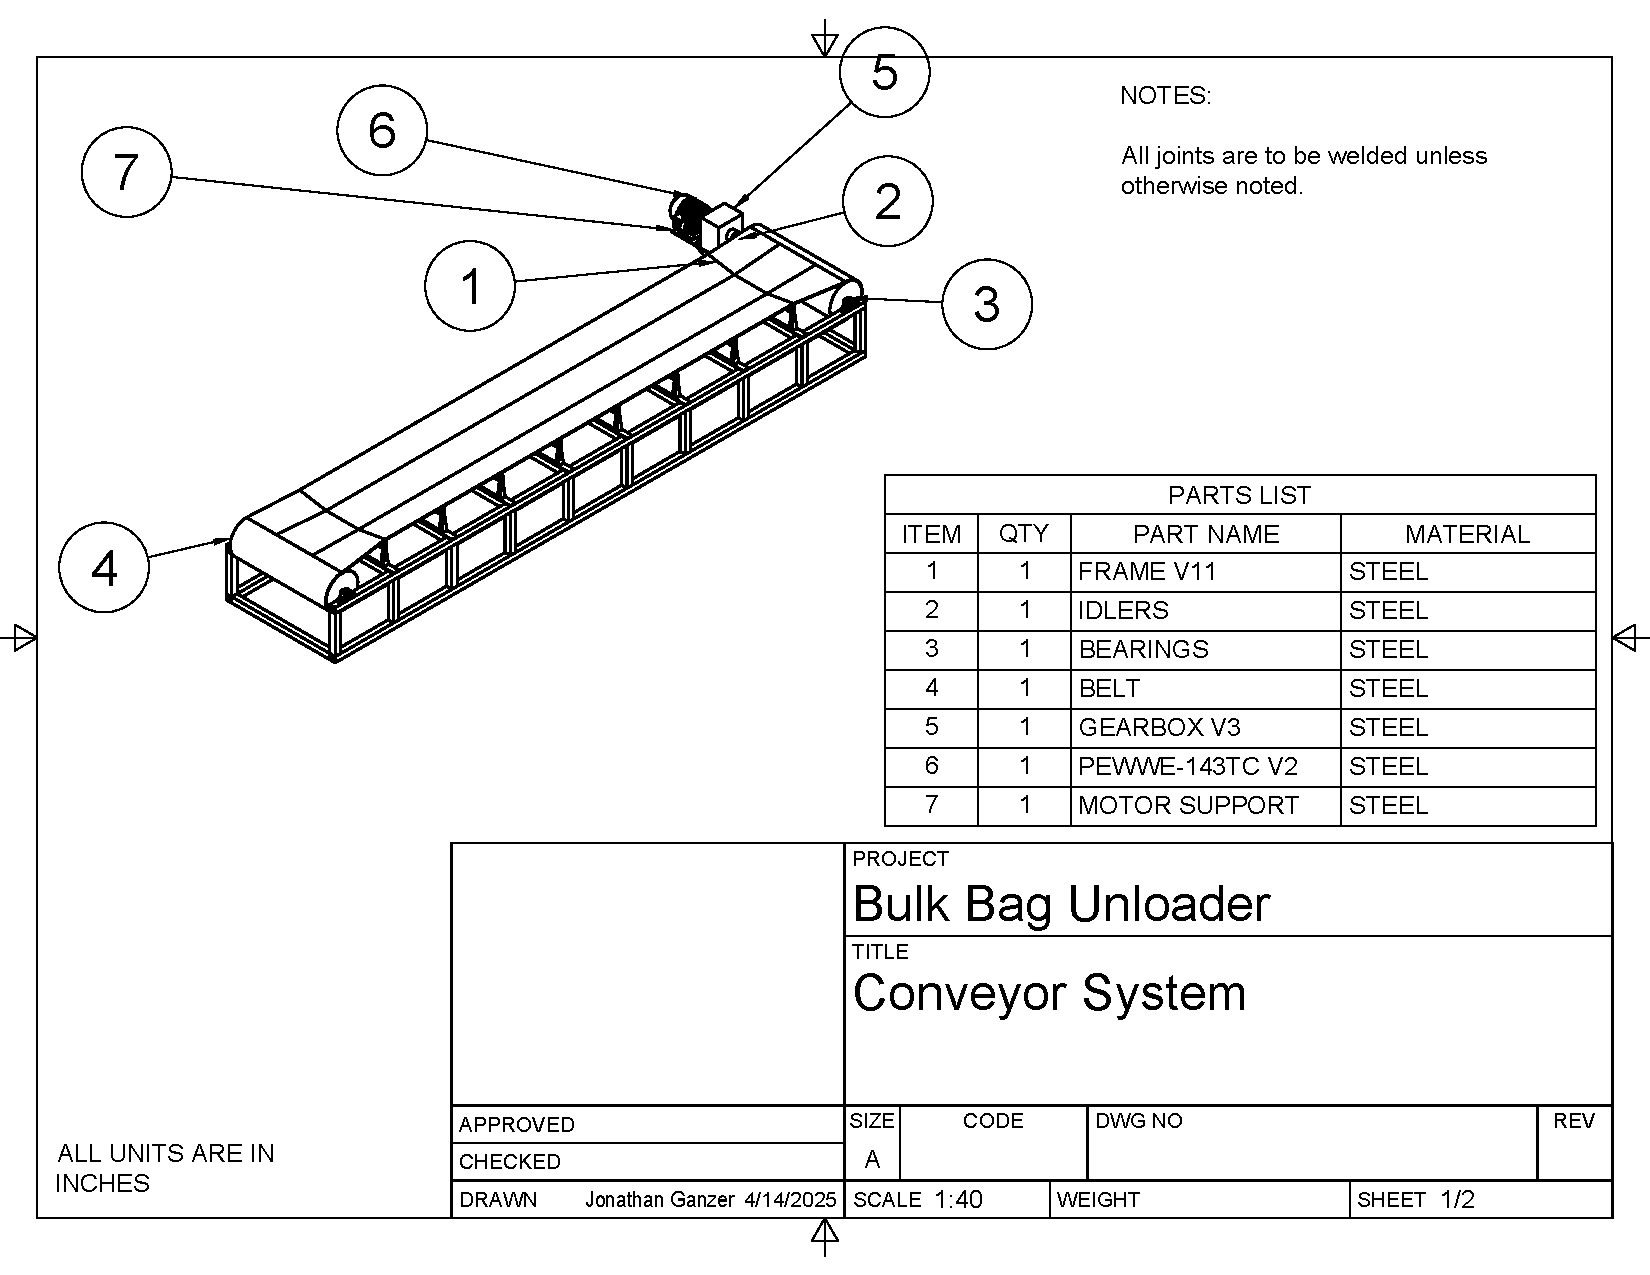
\includepdf[pages=-, fitpaper=true]{./Appendix/Conveyor/Conveyor System Drawings v3.pdf}
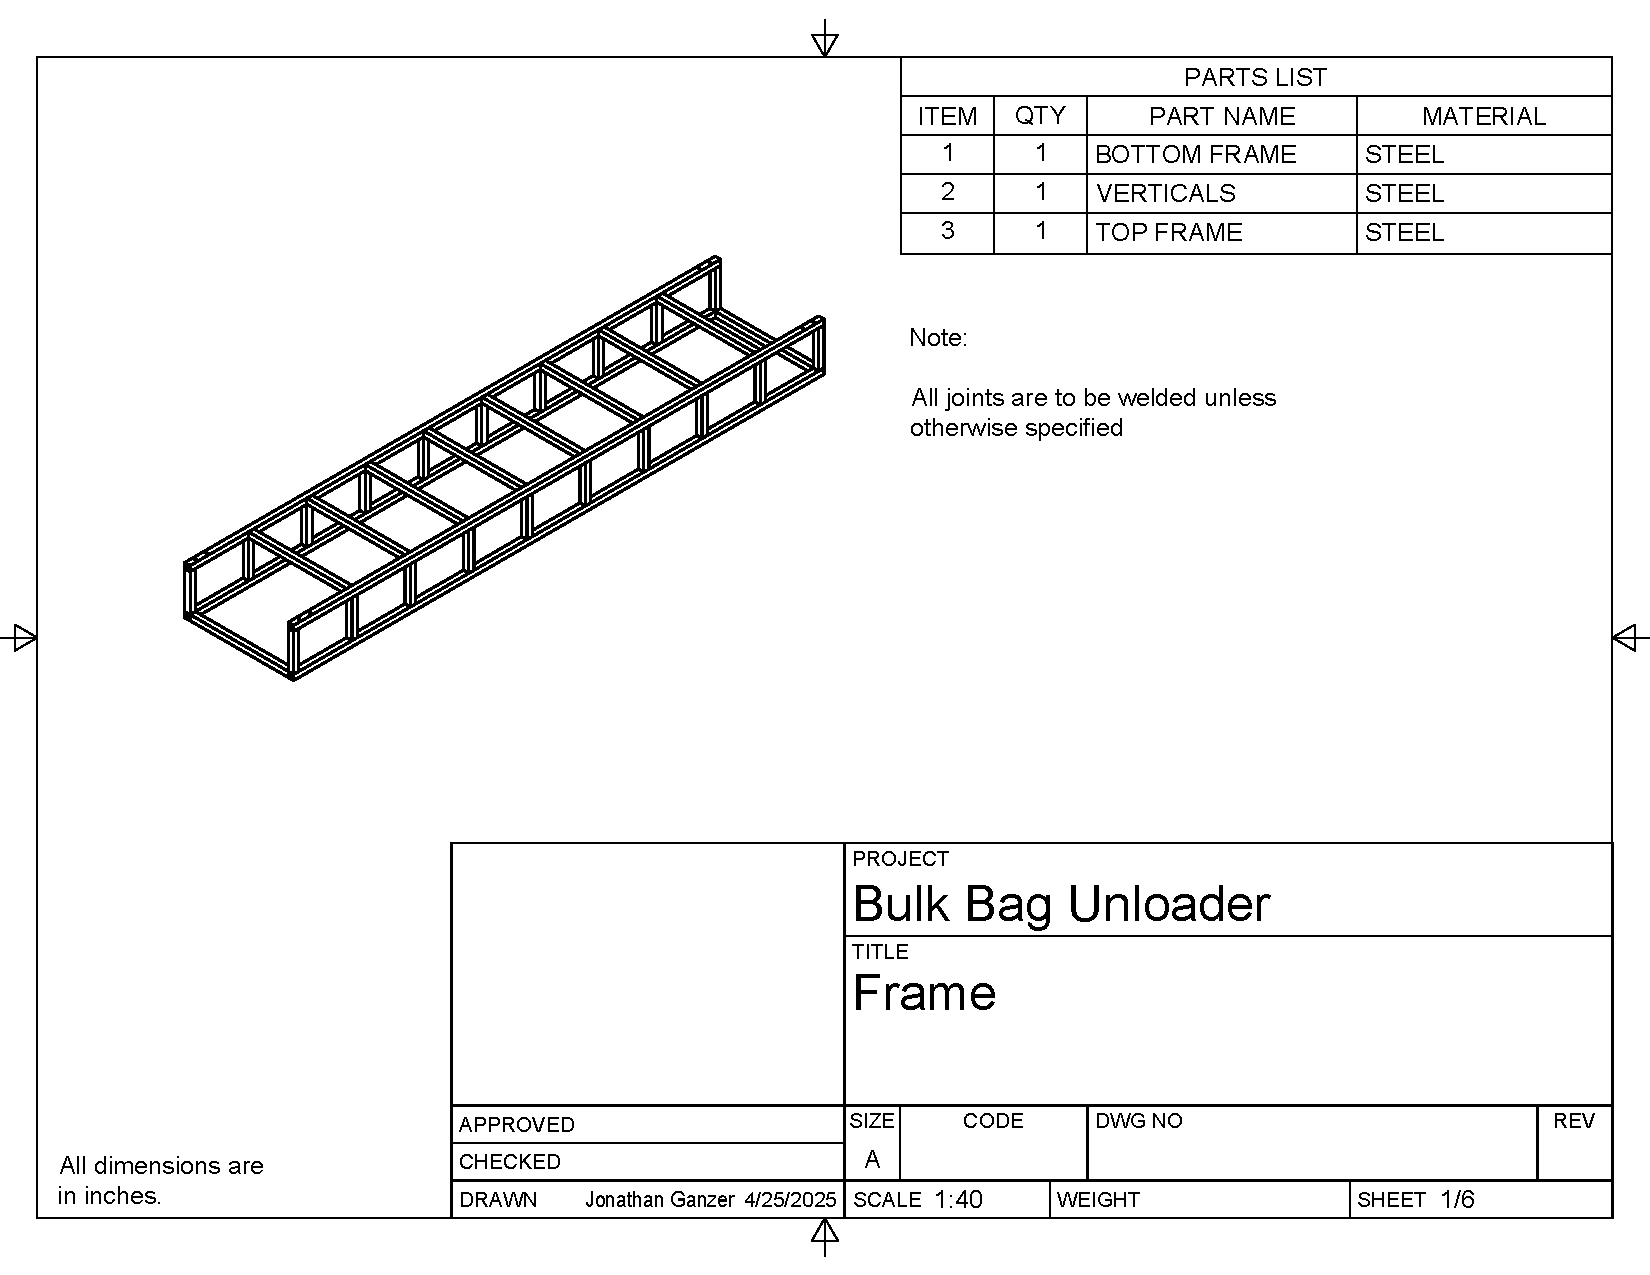
\includepdf[pages=-, fitpaper=true]{./Appendix/Conveyor/Frame Drawing v6.pdf}
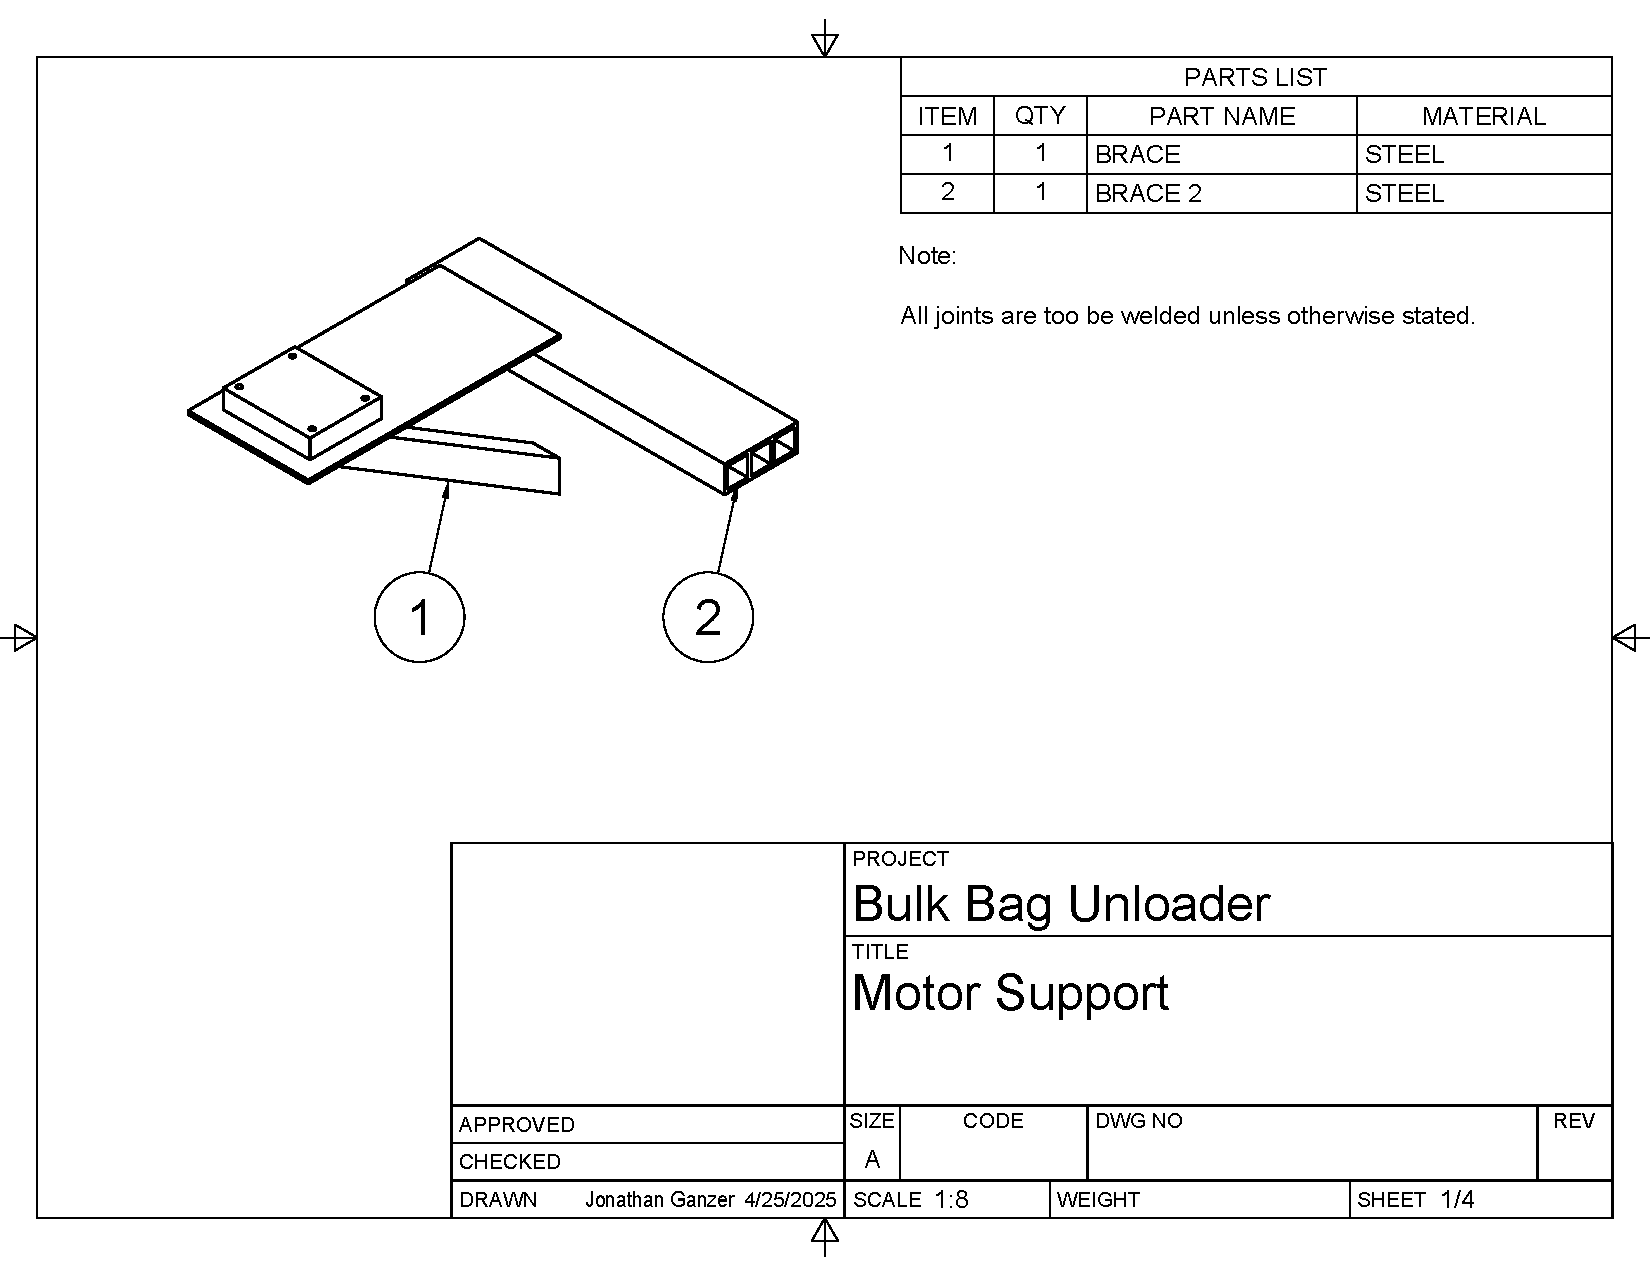
\includepdf[pages=-, fitpaper=true]{./Appendix/Conveyor/Motor Mount Drawing v7.pdf}
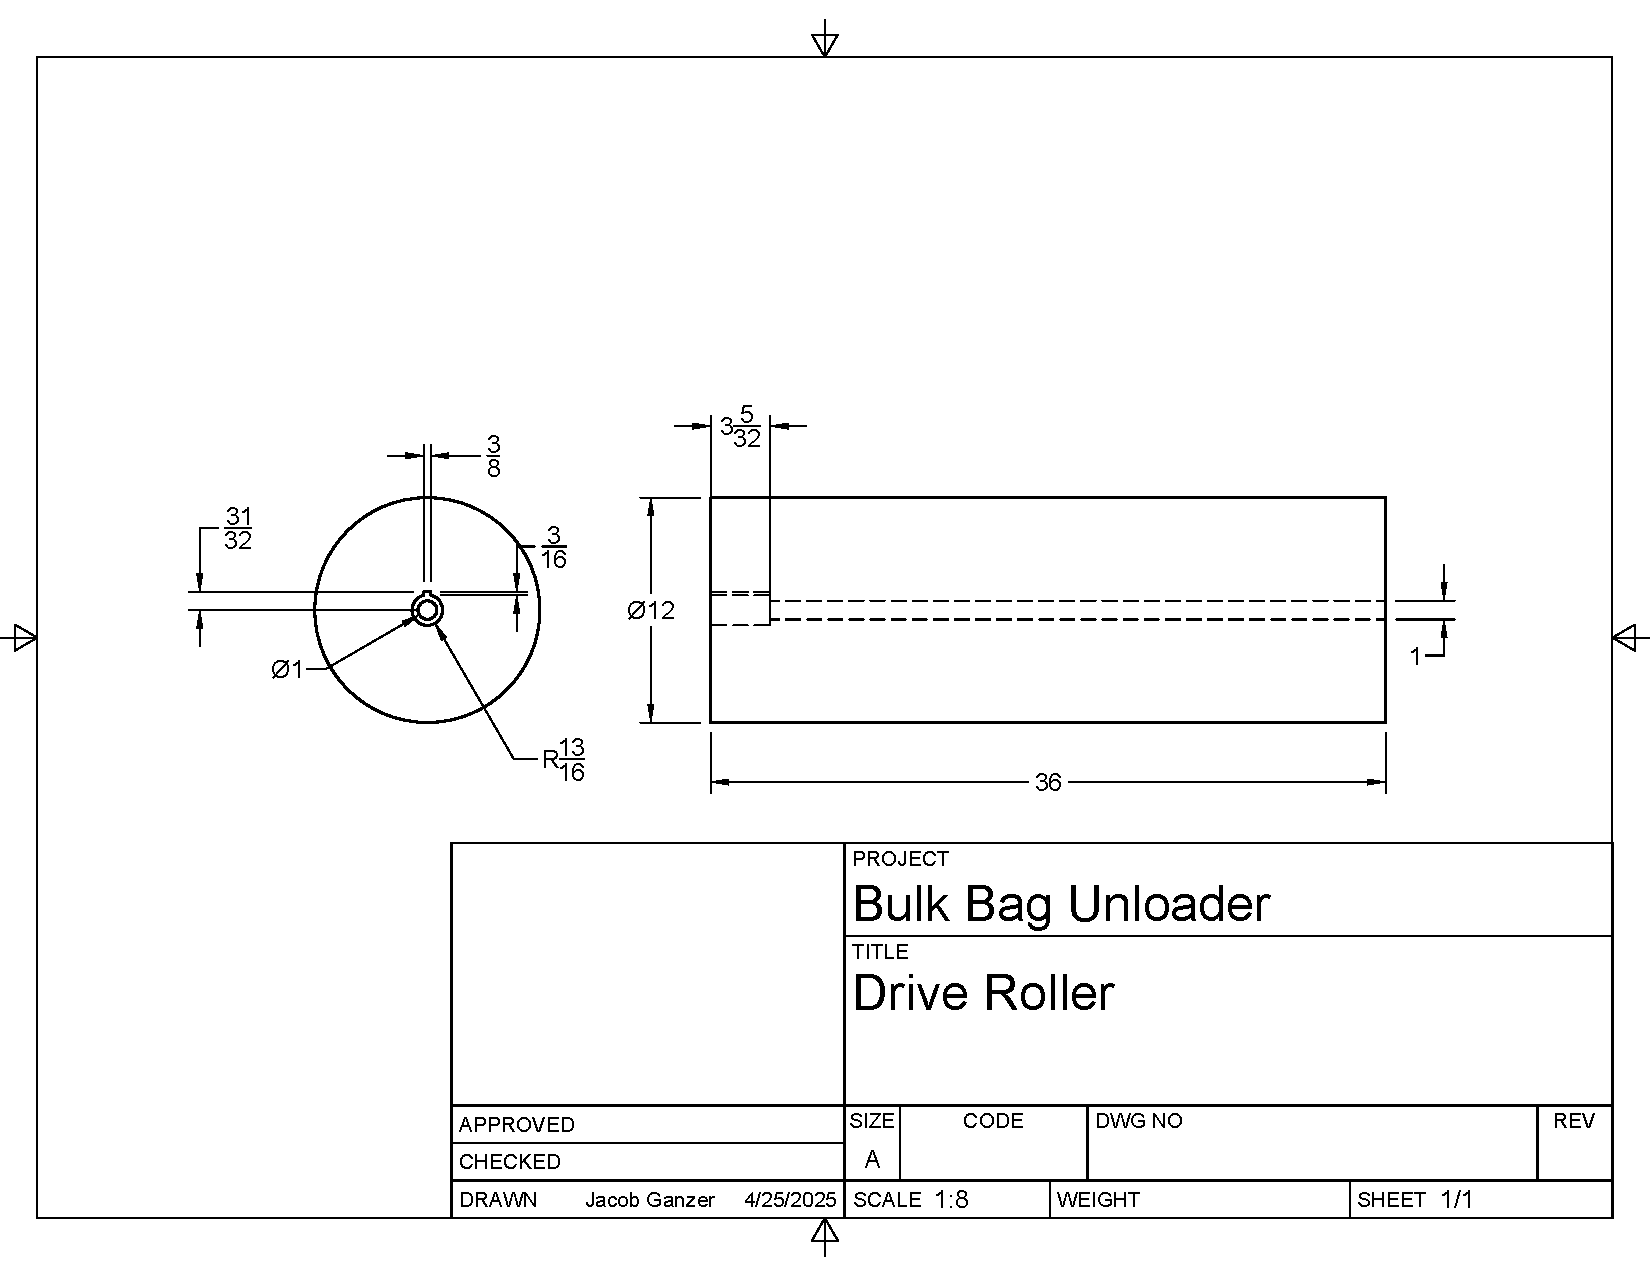
\includepdf[pages=-, fitpaper=true]{./Appendix/Conveyor/DriveRoller v1.pdf}
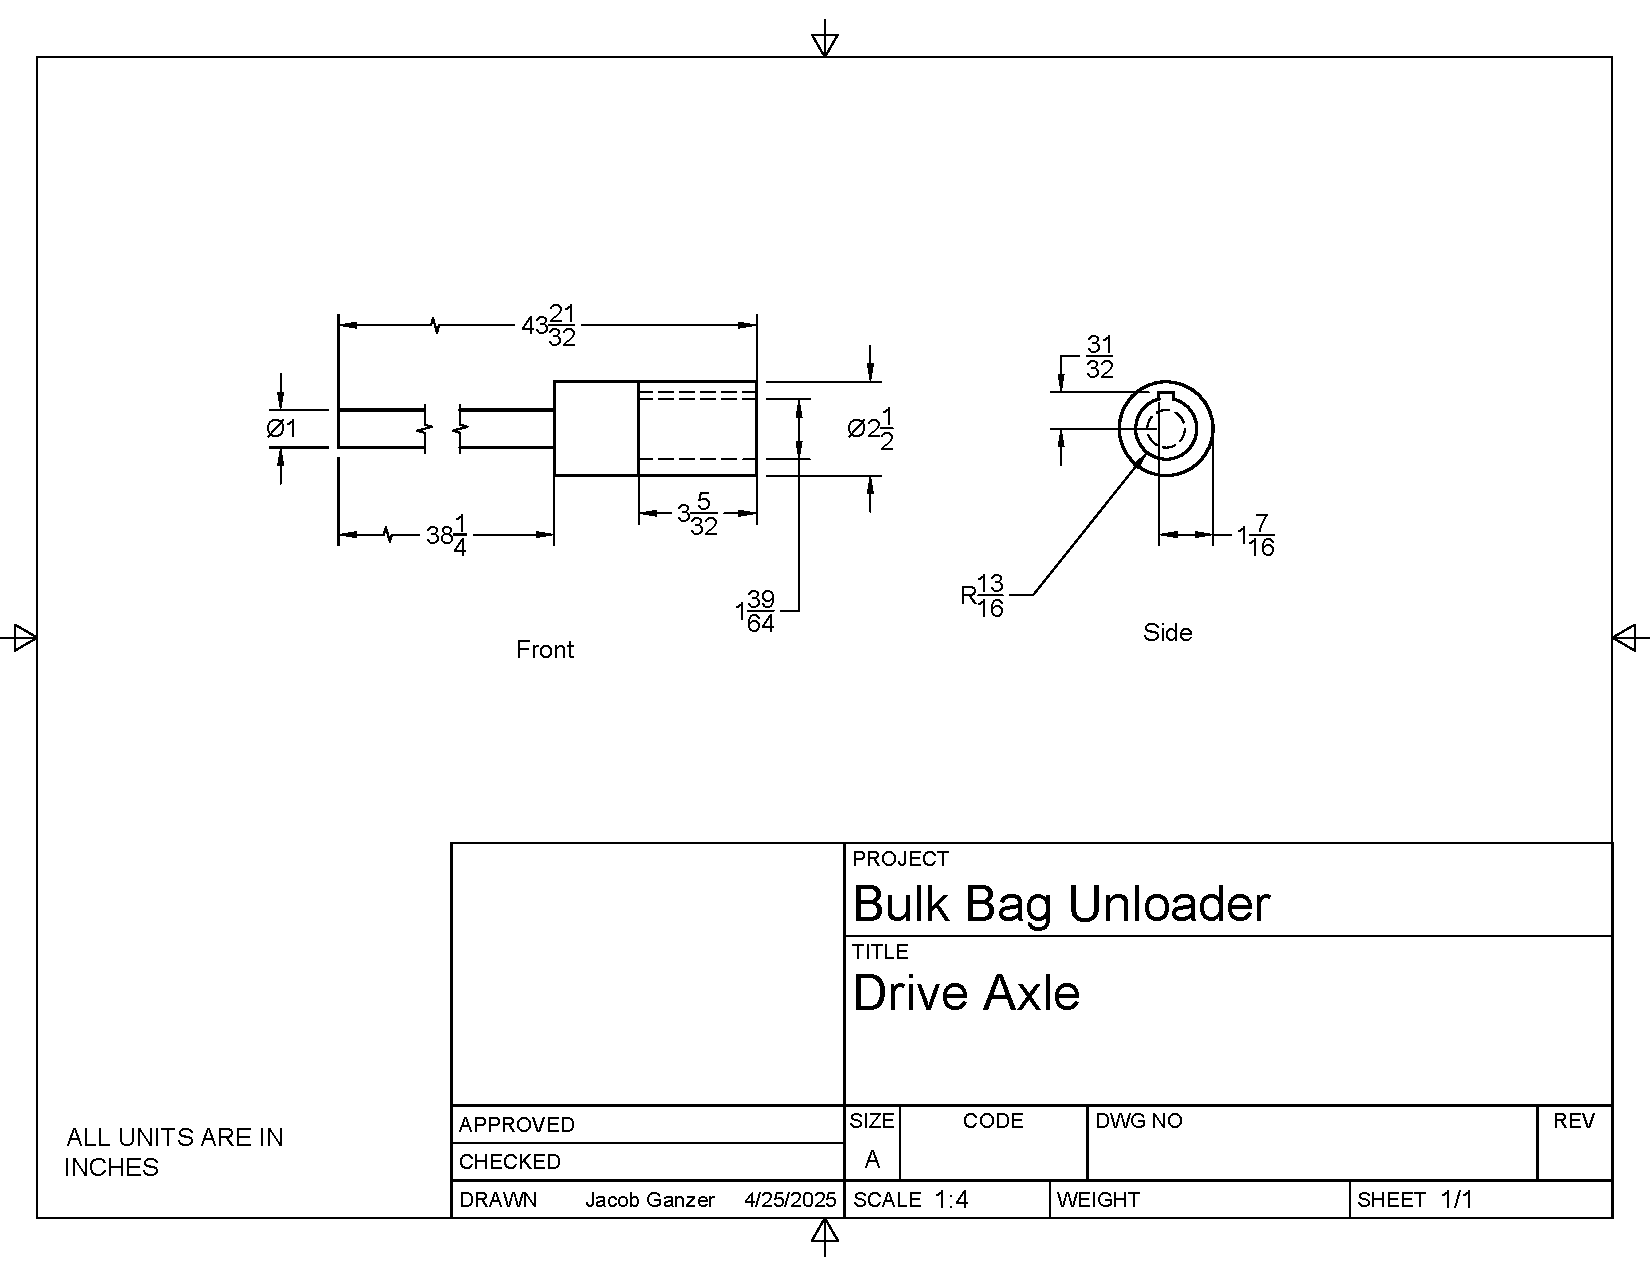
\includepdf[pages=-, fitpaper=true]{./Appendix/Conveyor/DriveAxle v4.pdf}
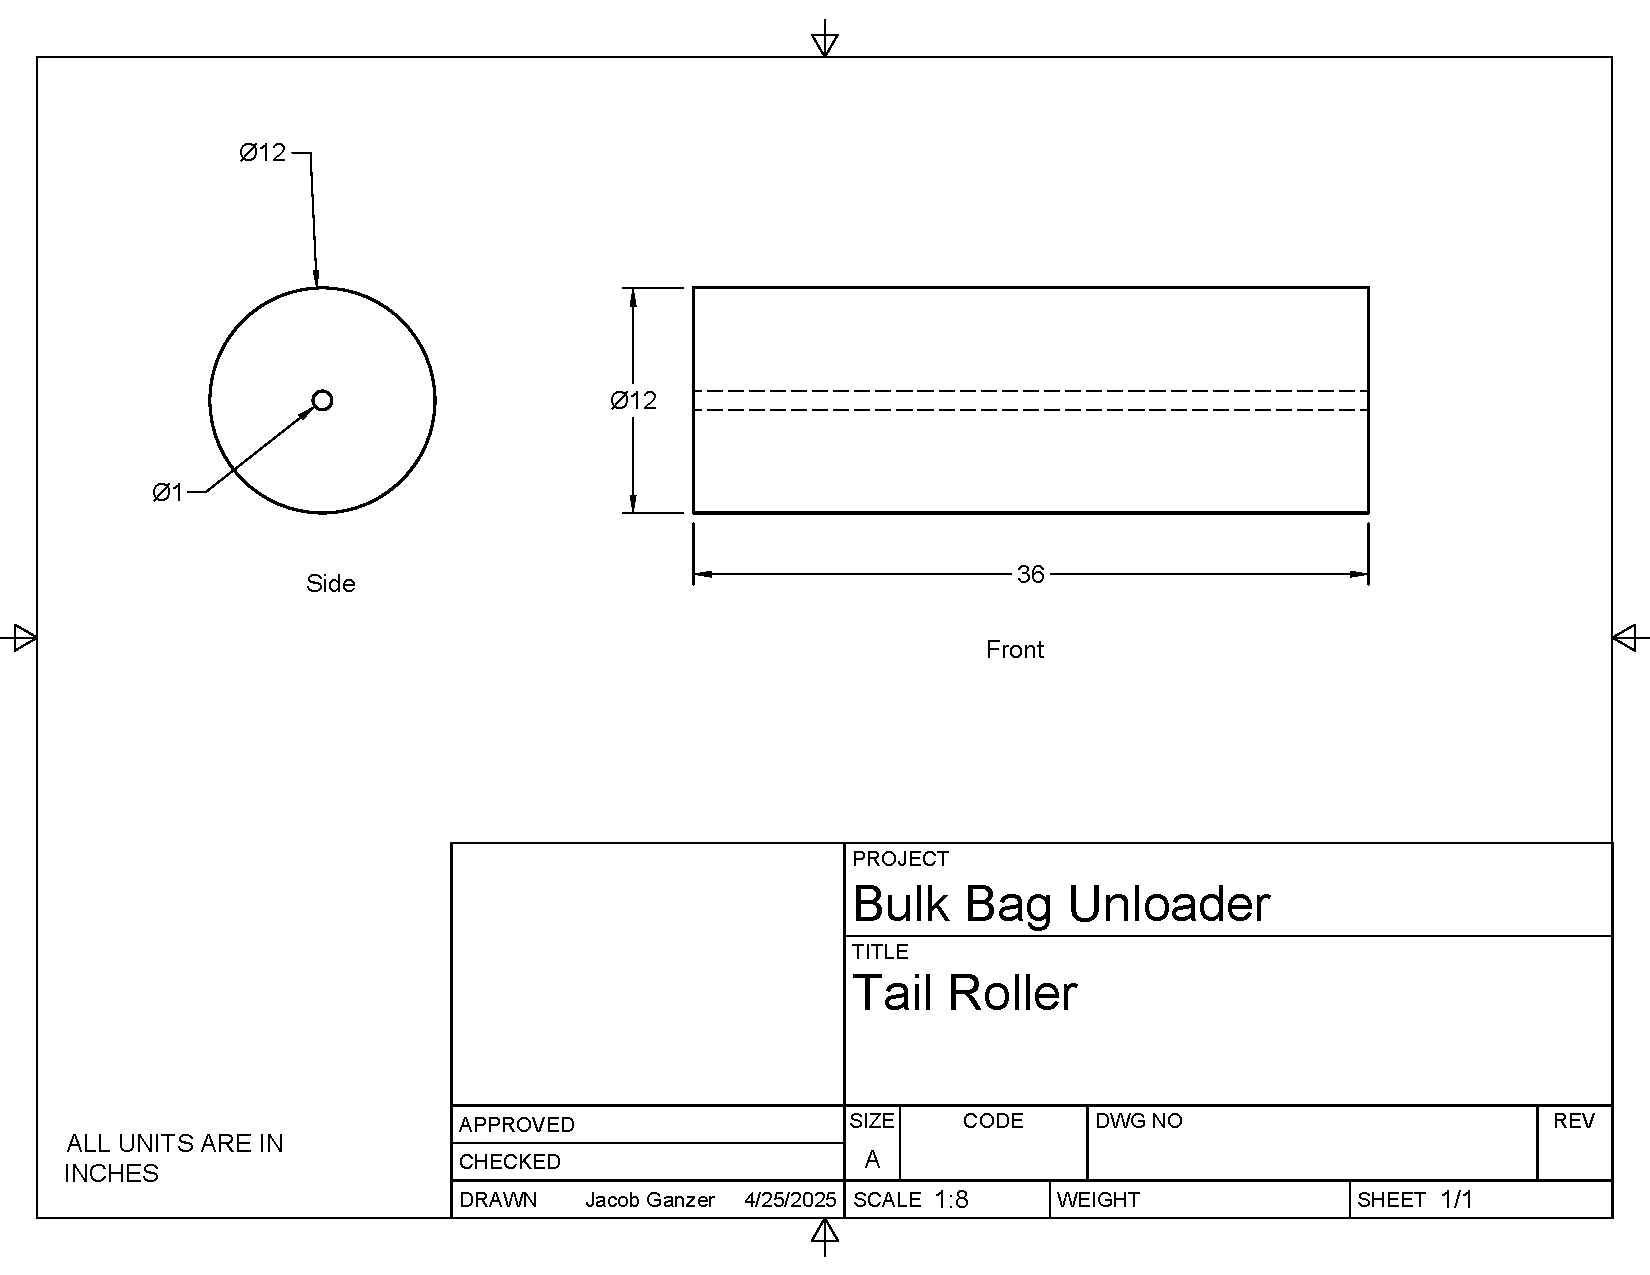
\includepdf[pages=-, fitpaper=true]{./Appendix/Conveyor/Tail Roller v3.pdf}
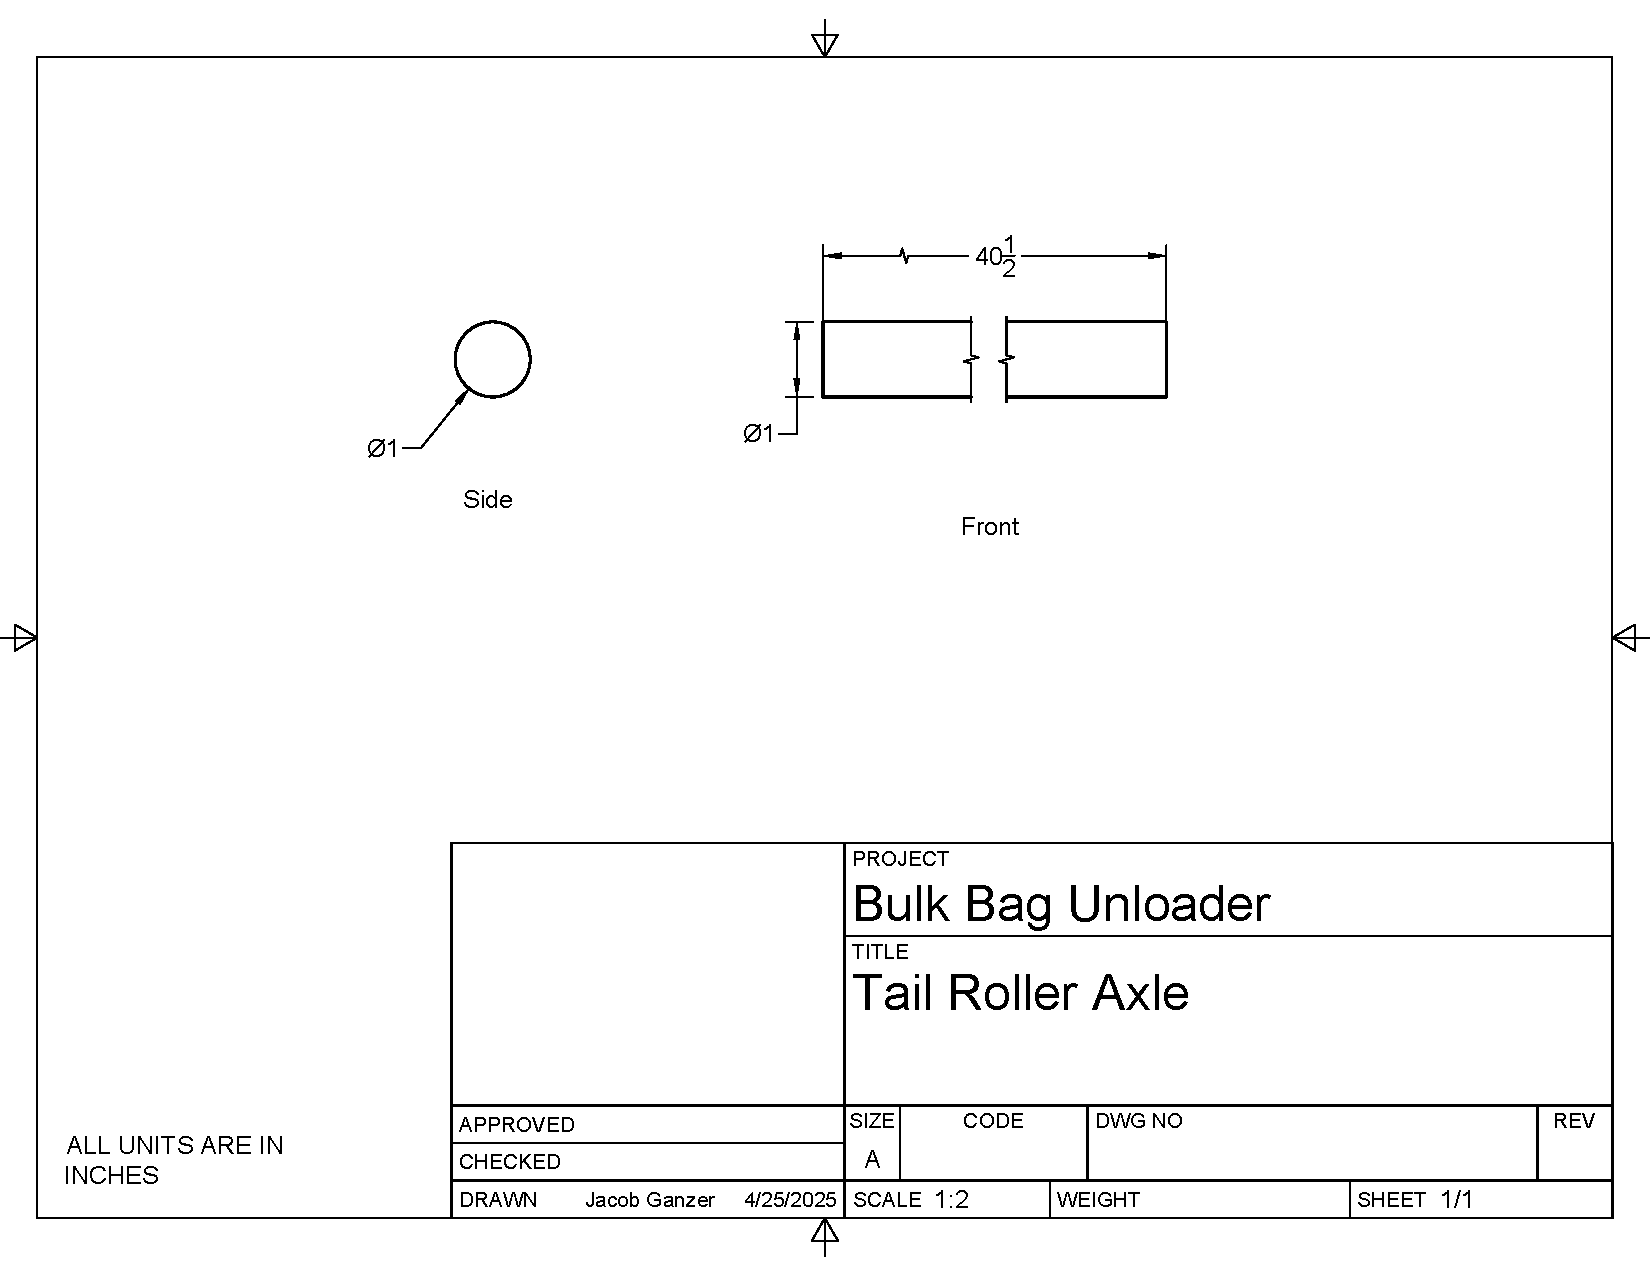
\includepdf[pages=-, fitpaper=true]{./Appendix/Conveyor/TailAxle v4.pdf}
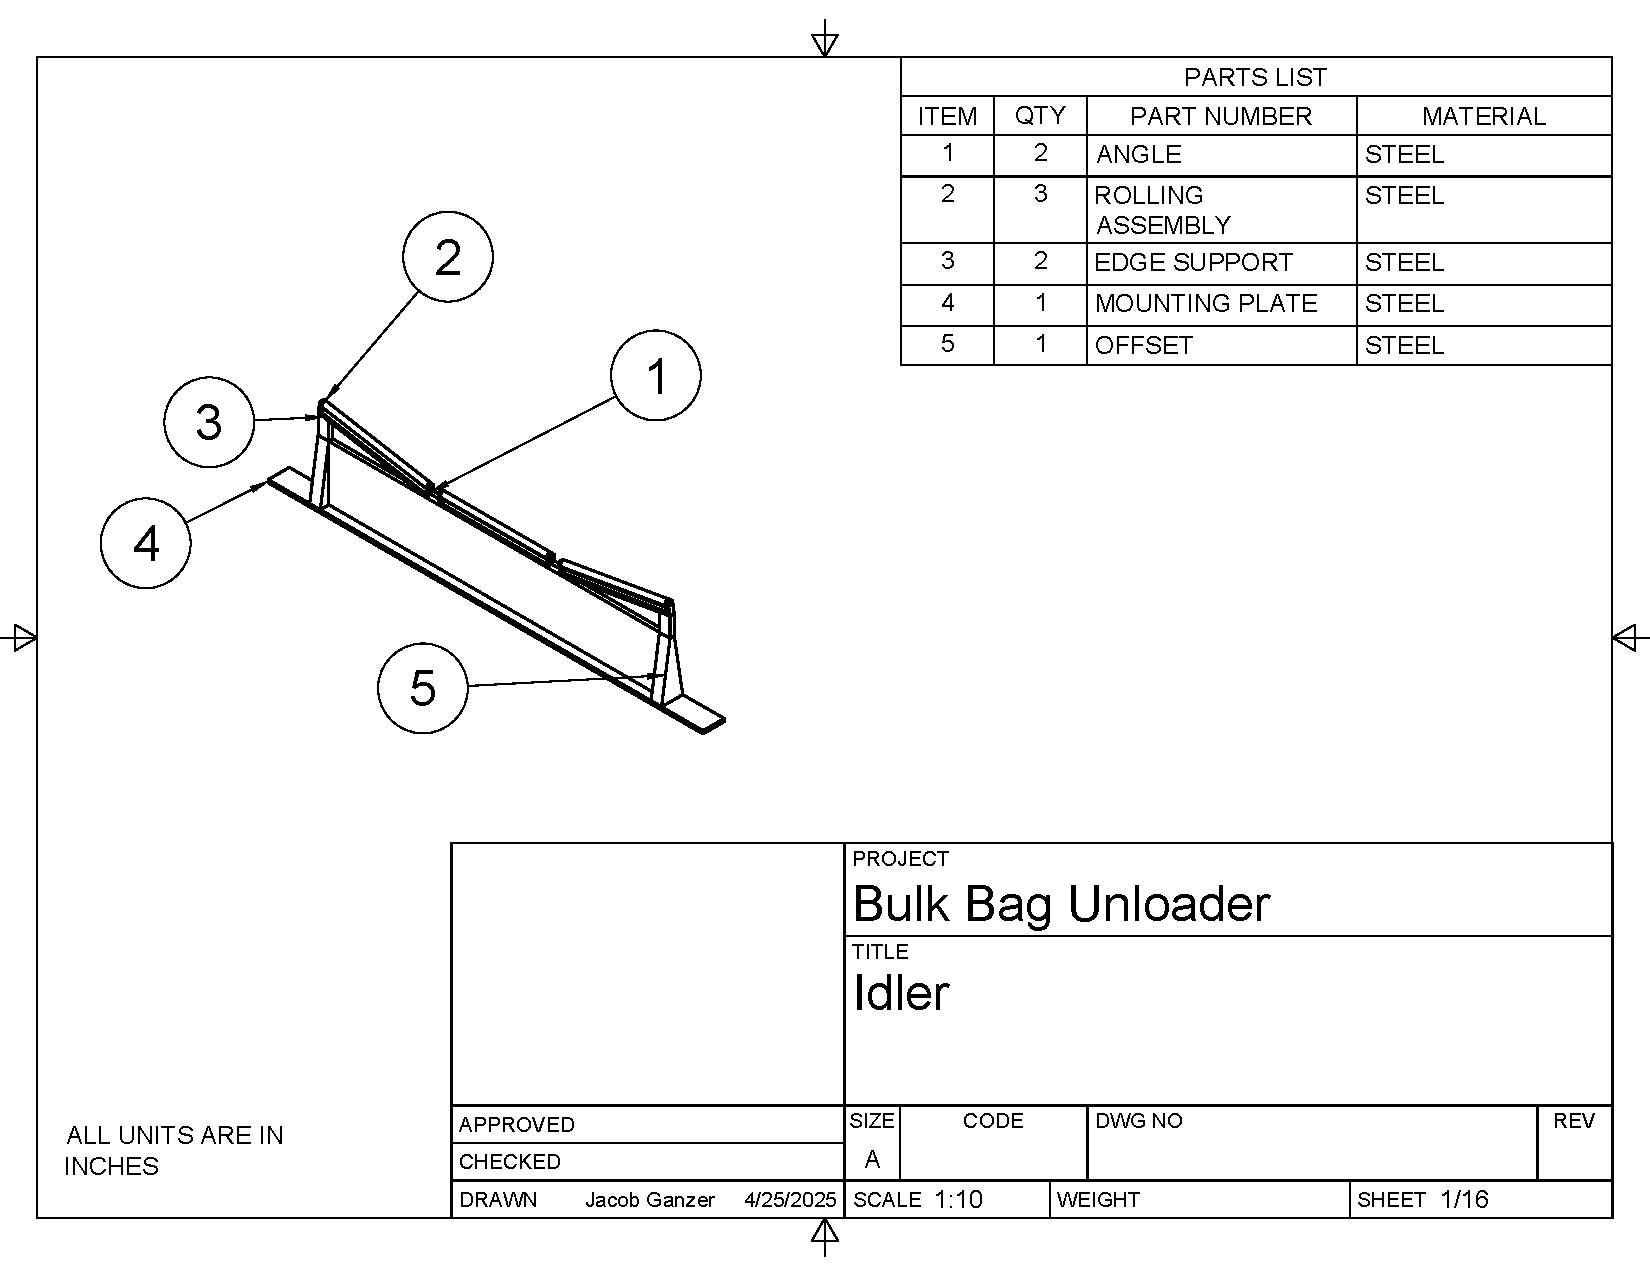
\includepdf[pages=-, fitpaper=true]{./Appendix/Conveyor/Idler v4.pdf}

\includepdf[pages=-, fatpaper=true]{./Appendix/Conveyor/7728T56_3D_Mounted Steel Ball Bearing with Cast Iron Housing}

\subsection{Mixing System}\label{pdf:mixer}
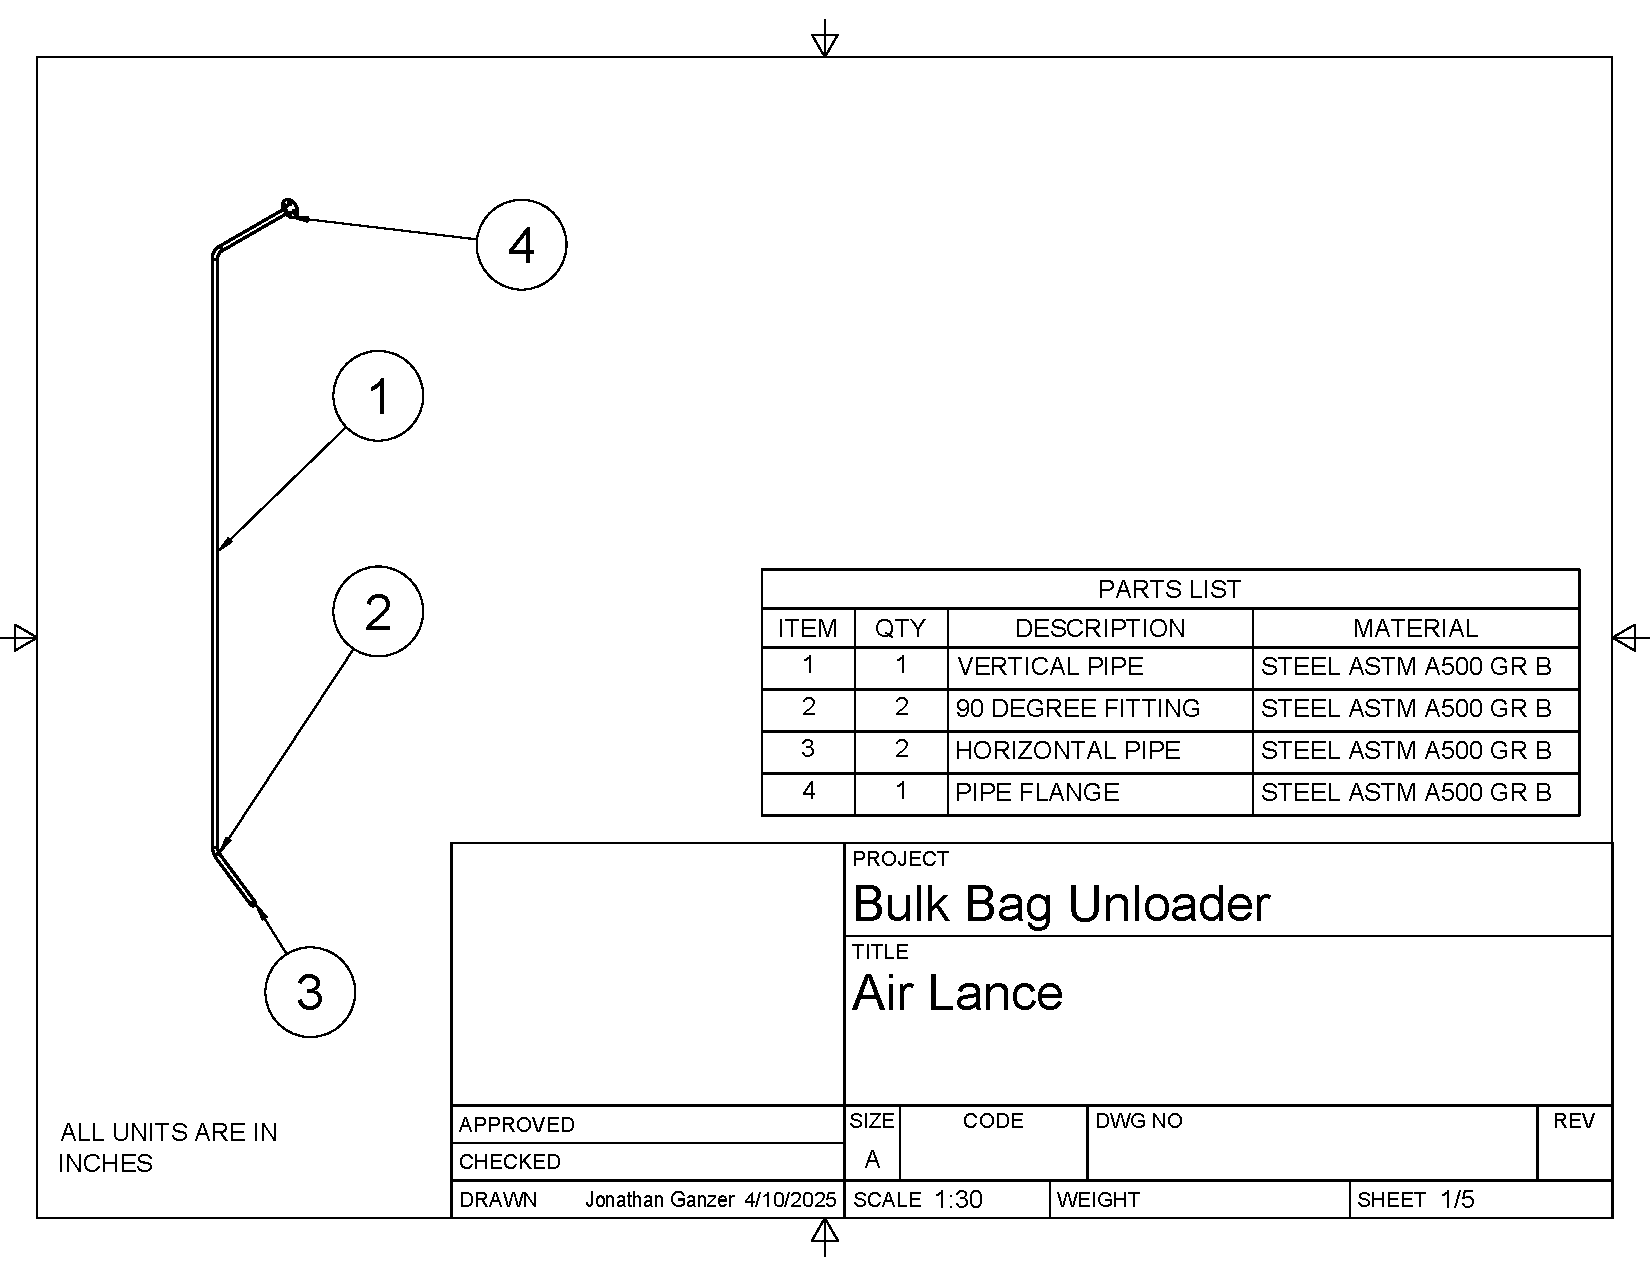
\includepdf[pages=-, fitpaper=true]{./Appendix/MixingSystem/Mixer Drawing v5.pdf}
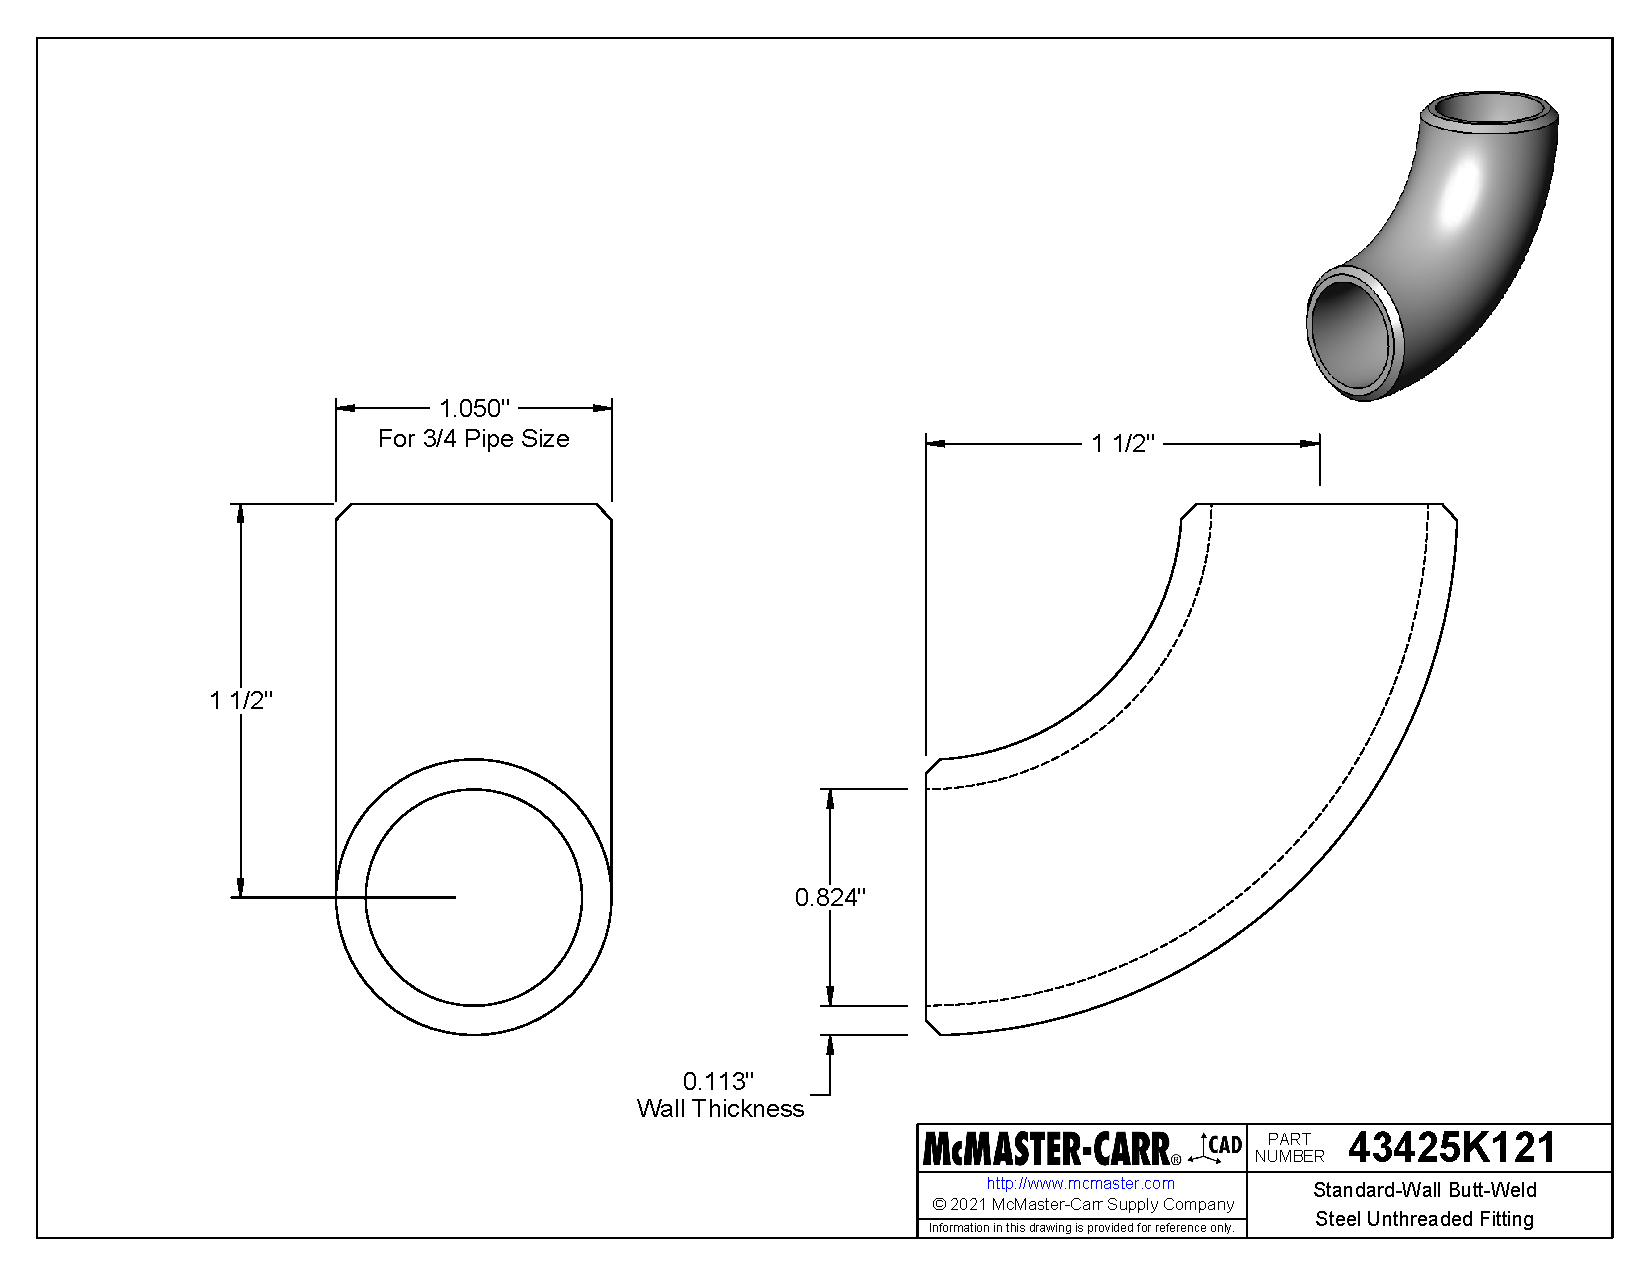
\includepdf[pages=-, fitpaper=true]{./Appendix/MixingSystem/43425K121_Standard-Wall Butt-Weld Steel Unthreaded Fitting.pdf}
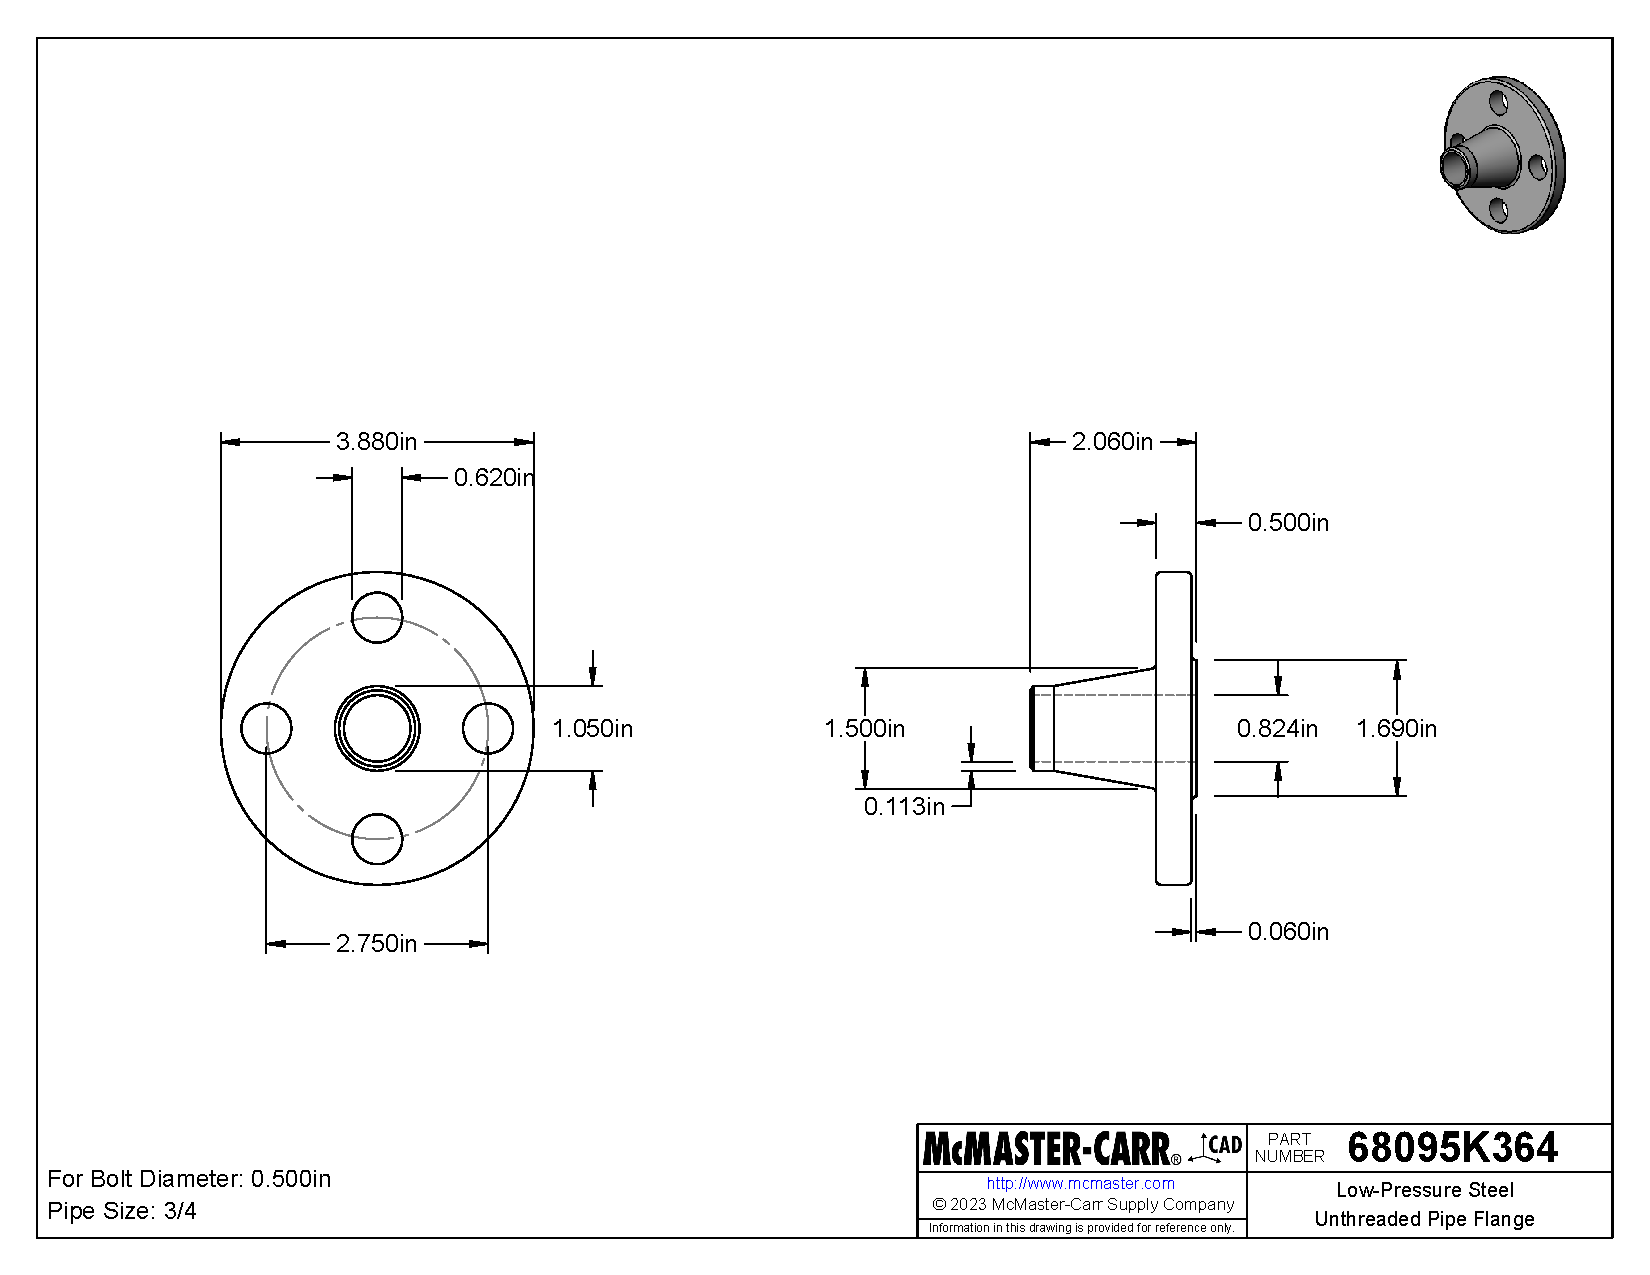
\includepdf[pages=-, fitpaper=true]{./Appendix/MixingSystem/68095K364_Low-Pressure Steel Unthreaded Pipe Flange.pdf}


\section{Author contributions}
%Writing of the final design report is intended to be shared by all team members. In this section put your name as the subsection heading and give a summary of what you contributed to the writing of the final design project report. 

\subsection{Gannon Steffes}

\begin{itemize}
    \item 1 - Wrote Introduction
    \item 1.1
    \item 1.2 - Wrote Introduction
    \item 1.2.1
    \item 1.3
    \item 1.4
    \item 2.2.1
    \item 2.2.2 - (Gannon and Ben)
    \item 2.2.3 - (Gannon and Ben)
    \item 3.1 - Work Breakdown Structure
    \item 3.2
    \item 4.2
\end{itemize}


\subsection{Benedict Brophy}
\begin{itemize}
    \item \ref{sec:elecspec}
    \item 1.5
    \item 2.2.0  
    \item 2.2.2 - (Gannon and Ben)
    \item 2.2.3 - (Gannon and Ben)
\end{itemize}


\subsection{Jacob Ganzer}
\begin{itemize}
    \item Abstract
    \item \ref{sec:pq} (Introduction)
    \item \ref{sec:transport}
    
    \item \ref{sec:mechDes}
    \item \ref{sec:mechbom}
    
    \item  \ref{sec:UnloadingSystem}
    \item \ref{sec:ConveyorSystem}
    \item \ref{sec:bulkbag}
    \item \ref{sec:ide} (Change from Grain Leg to Conveyor Belt)
    \item \ref{sec:designDev}
    \item \ref{sec:Material}
    \item \ref{sec:designUnload}
    \item \ref{sec:designBelt}
    \item \ref{sec:discuss}
    \item \ref{sec:future}
    \item \ref{sec:bulk}
    \item \ref{sec:demolish}
    \item \ref{sec:drawing}
    \item \ref{pdf:conveyor}

\end{itemize}


\subsection{Jonathan Ganzer}
\begin{itemize}
    \item \ref{sec:CaCl} - Adverse Reactions portion, Stainless Steel Cracking
    \item \ref{sec:HFAcid}
    %\item \ref{sec:transferMechanism}
    \item \ref{sec:UnloadingSystem}
    \item \ref{sec:ConveyorSystem}
    \item \ref{sec:MixingSystem}
    \item \ref{sec:GanttChart} - Introduction
    \item \ref{sec:Ideation-Mixer}
    \item \ref{sec:MixingSystemRefinement}}
   % \item \ref{sec:CADProgress}
    \item \ref{pdf:belt}
    \item \ref{pdf:conveyor}
    \item \ref{pdf:mixer}
\end{itemize}


\end{document}